% \documentclass[ebook,a4paper,12pt,oneside,openany]{memoir}
%\documentclass[10pt,oneside]{article}
\usepackage[bottom=2cm,top=2cm,left=2cm,right=2cm]{geometry}
\usepackage[utf8x]{inputenc}
\usepackage[english]{babel}
\usepackage{url}
\usepackage{amsmath, amssymb, amsthm}
\usepackage{indentfirst}
\usepackage{bm}
\numberwithin{equation}{chapter}
%\usepackage[tableposition=top]{caption}
\usepackage[num,abnt-emphasize=bf, bibjustif]{abntex2cite}
\usepackage{graphicx}
\usepackage[normalem]{ulem}
\usepackage[pdftex,colorlinks=true,citecolor=black,linkcolor=black,urlcolor=black,filecolor=black]{hyperref}
%-------------------------------
\usepackage{mathrsfs} %for mathscr chars {D, P, H}
%-------------------------------
\usepackage{booktabs,tabularx,ltablex} % breaking tables over several pages
%-------------------------------

%\usepackage{tipa}
\citebrackets[]

\DeclareMathOperator{\Tr}{Tr}

\def\mean#1{\left< #1 \right>}

\newcommand\bydef{\mathrel{\stackrel{\makebox[0pt]{\mbox{\normalfont\tiny def}}}{=}}}

% for placeholder text
%\usepackage{lipsum}

\documentclass[ebook,a4paper,12pt,oneside,openany]{memoir}
%\documentclass[10pt,oneside]{article}
\usepackage[bottom=2cm,top=2cm,left=2cm,right=2cm]{geometry}
\usepackage[utf8x]{inputenc}
\usepackage[english]{babel}
\usepackage{url}
\usepackage{amsmath, amssymb, amsthm}
\usepackage{indentfirst}
\usepackage{bm}
\numberwithin{equation}{chapter}
%\usepackage[tableposition=top]{caption}
\usepackage[num,abnt-emphasize=bf, bibjustif]{abntex2cite}
\usepackage{graphicx}
\usepackage[normalem]{ulem}
\usepackage[pdftex,colorlinks=true,citecolor=black,linkcolor=black,urlcolor=black,filecolor=black]{hyperref}
%-------------------------------
\usepackage{mathrsfs} %for mathscr chars {D, P, H}
%-------------------------------
\usepackage{booktabs,tabularx,ltablex} % breaking tables over several pages
%-------------------------------

%\usepackage{tipa}
\citebrackets[]

\DeclareMathOperator{\Tr}{Tr}

\def\mean#1{\left< #1 \right>}

\newcommand\bydef{\mathrel{\stackrel{\makebox[0pt]{\mbox{\normalfont\tiny def}}}{=}}}

% for placeholder text
%\usepackage{lipsum}


%%%%%%%%%%%%%%%%%%%%%%%%%%%%%%%%%%%%%%%%%%%%%%%%%%%%%%%%%%%%%%%%%%%%%%%%%%
%% To do List:								%%
%% - Table of equations at the end of the e-book - Plinio		%%
%% - Correct some items in the Bibliography - Plinio			%%
%% - Re-write Section 1.1 (out of date) - Ximenes			%%
%% - Write Section 2.8 and correct the sections that uses it - Plinio	%%
%% - Write Section 3.3 and correct the sections that uses it - Plinio	%%
%%%%%%%%%%%%%%%%%%%%%%%%%%%%%%%%%%%%%%%%%%%%%%%%%%%%%%%%%%%%%%%%%%%%%%%%%%

\title{An Introduction to the Physics\\ of Electron Storage Rings}
\author{M. Sands}

\begin{document}
\maketitle
\vspace{30mm}
\begin{flushright}
    \textit{Author:} \\
    \vspace{1mm}
        Matthew Sands \\
    \vspace{5mm}
    \textit{Adaptation by:} \\
    \vspace{1mm}
	Pl\'inio S. Dester \\
	Isabella Stevani \\
	Ximenes Resende \\
  Fernando de S\'a \\
  Murilo B. Alves \\
\end{flushright}

\thispagestyle{empty}

\newpage
\tableofcontents

\newpage
\begin{center}
	\textbf{\large Most commonly used symbols.}
\end{center}

\begin{tabularx}{\linewidth}{@{}lX@{}}
	$A$			& Area of a transverse section of a stored beam; or amplitude of an oscillation.\\
%   $A_\text{int}$ & An effective area of colliding beams.\\
	$a$			& Amplitude of an oscillation; invariant part of an amplitude.\\
    $\alpha$	& Time dilation of dispersion orbits (momentum compaction).\\
	$\alpha_i$	& Damping coefficients of oscillations ($1/\tau$); $i = x, z, \epsilon$.\\
    $B$			& Magnetic field strength.\\
	$\beta(s)$	& Betatron functions.\\
	$c$			& Speed of light.\\
	$\gamma$	& Energy in units of rest energy ($E/mc^2$).\\
	$D$			& %Electron number per unit area ($N/A$); or
    				rate of change of radiationloss with energy ($dU/dE$).\\
%	$\delta$	& Half of the angle of intersection of colliding beams.\\
	$E$			& Electron energy.\\
    $E_0$		& Nominal energy of a stored beam.\\
    $\mathscr{E}$ & Electric field strength.\\
    $e$			& Electric charge of an electron.\\
	$\epsilon$	& Energy deviation ($E - E_0$).\\
    $f$			& Frequency of revolution of a synchronous electron ($c/L$).\\
    $G(s)$		& Curvature function of the design orbit ($1/\rho_s$).\\
    $G_0$		& Curvature of the design orbit of an isomagnetic guide field ($G_0 = 1/\rho_0$).\\
	$\zeta(s)$	& Envelope function ($\sqrt{\beta(s)}$).\\
    $\eta(s)$	& Dispersion function.\\
%   $h$			& Beam height.\\
%	$h^*$		& Beam height at the intersection.\\
%	$I$			& Beam current (Nef).\\
	$J_i$		& Partition numbers of the damping rates; $i = x, z, \epsilon$.\\
    $K(s)$		& Focusing functions of the guide field.\\
	$k$			& Rf harmonic number ($\omega_\text{rf}/\omega_\text{r}$); or deviation from nominal value of a focusing function ($\Delta K$).\\
    $L$			& Length of the design orbit ($c/f$).\\
    $\ell$		& Trajectory length.\\
    %; bunch length.\\
    $m$			& Rest mass of an electron.\\
    $N$			& Number of stored electrons in a beam.\\
    %($I/ef$).\\
	$\nu$		& Betatron number.\\
%	$\Delta \nu_0$ & Beam-beam interaction parameter.\\
	$P$			& Radiofrequency power.\\
    $p$			& Electron momentum.\\
%	$Q$			& Quantum excitation strength.\\
	$q$			& Rf overvoltage ($eV/U_0$).\\
%	$R$			& Gross radius of the design orbit ($L/2\pi$).\\
	$r_e$		& Classical electron radius ($e^2/4\pi\epsilon_0 m c^2$).\\
    $\rho_s$	& Radius of curvature of the design orbit at $s$ [$1/G(s)$] .\\
    $\rho_0$	& Magnetic radius in an isomagnetic guide field.\\
	$s$			& Azimuthal (longitudinal) coordinate.\\
    $\sigma$	& Standard deviation of a distribution.\\
	$T(\epsilon)$ & Time for a revolution.\\
	$T_0$		& Revolution period of a synchronous electron ($L/c$).\\
	$t$			& Laboratory time.\\
	$\tau$		& Time displacement between an electron and the center of its bunch ($y/c$).\\
	$\tau_i$	& Damping time constant of an oscillation mode ($i/\alpha_i$); $i = x,z,\epsilon$.\\
	$\varphi(s)$ & Phase variable of betatron oscillations.\\
	$\Phi(\tau)$		&  Pseudopotential energy of the longitudinal oscillations.\\
	$U(\epsilon)$ & Energy loss by radiation in one revolution.\\
	$u$			& Energy of a radiated quantum.\\
	$V(\tau)$	& Effective "Voltage" of the rf system.\\
%	$w$			& Beam width.\\
%	$w^*$		& Beam width at the intersection.\\
	$x$			& Horizontal (radial) displacement from the design orbit.\\
	$y$			& Longitudinal (azimuthal) displacement from a bunch center $(c\tau)$.\\
    $z$			& Vertical (axial) displacement from the design orbit.\\
    $\Omega$	& Angular frequency of the energy (and longitudinal) oscillations.\\
    $\omega_r$	& Angular frequency of revolution ($2\pi/T_0$).\\
	$\omega_\beta$ & Angular frequency of a betatron oscillation ($\nu\omega_r$).
\end{tabularx}


\chapter{Introduction} \label{ch:1}
    \section{Opening Remarks}

% Electron storage rings have now come of age. With the successful operation of Adone, experiments will now begin using colliding beams of electrons and positrons with energies of 1 GeV and beyond, expanding the area of storage ring research which was begun at lower energies with the pioneering instruments at Stanford, Frascati, Novosibirsk, and Orsay. Projects under way at Novosibirsk, Cambridge, electrons Hamburg, and Stanford will soon provide stored colliding beams of electrons at even higher energies. Larger numbers of workers will be basing their research in particle physics on these instruments. Many of the physicists who will be using storage rings will not have had a part in their design and construction, and will not initially have a knowledge of their inner workings. The aim of this report is to provide for such physicists a review of basic of the basic physical processes that determine the behavior of electron storage rings -- with a particular concern for their performance as instruments for research in particle physics. Because of this aim, the material is generally not presented in the form which might be most convenient for those who will be interested in the design of storage rings. It is, rather, developed in a form intended to give the using physicist an understanding of the inherent properties of his instrument -- especially those which will have an influence on his observations -- and to give him some feeling for its basic limitations and its ultimate capabilities.

% In the rest of this introduction I give a qualitative description of each of the basic phenomena that play a role in colliding beam storage rings, including a discussion of the factors which determine the luminosity. This first part is intended to provide a background and a vocabulary for the appreciation of the other reports which describe the operating experience with existing rings and the projects for new rings. In the remaining parts I shall consider in detail the theory of those basic single particle processes which determine the ultimate limits on the performance of storage rings. A discussion of the important collective effects, which have lead to many practical difficulties in high intensity rings, is not included here, but will de found in the report of Pellegrini. At the end, I return to a discussion of the limitations on the performance of high energy storage rings, and apply the results to an illustrative example -- the new Stanford design for a 2-3 Gev ring.

    \section{Basic Processes}\label{sec:1.2}

Let us begin with a brief qualitative description of the basic processes which come into play in producing a stored electron beam. (See Fig.~\ref{fig:ring})

\begin{figure}[!htb]
	\centering
	
\includegraphics[width=0.6\linewidth]{./Figuras/placeholder.png}
	\caption{Schematic diagram of an electron storage ring.}
	\label{fig:ring}
\end{figure}

A short pulse of a beam of electrons is injected into a vacuum chamber embedded in a more-or-less circular \emph{magnetic guide field}. The guide field leads the electrons around in more-or-less closed paths to make a \emph{stored beam}.

The guide field has \emph{focussing} properties which drive all electrons toward an ideal \emph{design orbit} and cause them to execute lateral (radial and vertical) \emph{betatron oscillations} about the ideal closed path.

During each revolution an electron loses a small fraction of its energy by \emph{synchrotron radiation}. For stored electrons this energy loss is compensated for by a corresponding gain of energy from a radio frequency cavity (or from several cavities acting in concert).

The periodic accelerating field collects the electrons into circulating \emph{bunches}, within which the individual electrons oscillate in \emph{longitudinal} position and in energy relative to an ideal reference particle at the center of the bunch. The associated motions in longitudinal position and energy are called the \emph{synchrotron oscillations}.

The energy loss by synchrotron radiation together with the compensating energy gain from the rf cavity gives rise to a slow \emph{radiation damping} of all oscillation amplitudes; the trajectory of each electron tends toward that of an ideal reference particle at the center of the bunch (which moves with constant speed along the design orbit).

Radiation damping does not conserve phase density, so it is possible to inject, successively, many pulses into the neighborhood of the same ideal orbit and obtain high circulating currents from weak sources.

The damping of all oscillation amplitudes is effectively arrested because of a continuous excitation of the oscillations by “noise” in the electron energy, which comes about from the fact that the synchrotron radiation is emitted in photons of discrete energy - the so-called \emph{quantum fluctuations} of the energy loss.

In stationary conditions a balance is reached between quantum excitation and radiation damping, leading to a statistically stationary distribution of the oscillation amplitudes and phases of the electrons in a bunch. The bunch then takes on the aspect of a traveling strip of ribbon which has a stationary “size” and “shape”, with a Gaussian distribution of amplitudes in each of the transverse and longitudinal coordinates (see Fig.~\ref{fig:fig2}). (The shape of a bunch will be different at each azimuthal position because the focussing properties of the guide field vary from place to place, but in the stationary condition the bunch has the same transverse shape at each successive turn for any chosen azimuth).

\begin{figure}[!htb]
	\centering
	
\includegraphics[width=0.55\linewidth]{./Figuras/placeholder.png}
	\caption{Circulating bunches in a stored beam.}
	\label{fig:fig2}
\end{figure}

-- For each coordinate of an electron there is some maximum oscillation amplitude above which the electron no longer remains captured in the bunch. We may refer to the range of stable amplitude in each coordinate at its \emph{aperture}. An electron is lost from a bunch when some disturbance increases the amplitude in any coordinate beyond the corresponding aperture limit. The aperture limit for each coordinate may be set by.a physical obstacle which intercepts the electrons, or by nonlinear effects in the focussing forces which lead to unbounded trajectories for large displacements from the ideal reference electron.

-- Electrons may be lost by scattering or energy loss in collisions with molecules of the residual gas in the vacuum chamber, or by a large statistical fluctuation in the quantum excitation of an oscillation amplitude.

The basic processes considered above are the single-particle effects which are primarily responsible for the intrinsic properties of a stored electron beam. Until now I have considered a bunch as a collection of noninteracting electrons each of which moves as though it were alone in the storage ring. Unfortunately,life is not so simple.
    \section{Collective Effects} \label{sec:1.3}
When the number of electrons in a circulating bunch is large enough (typically, greater than 10$^9$ or so) interactions \emph{among} the electrons of a bunch, or among bunches, become important - and have, in fact, been a serious problem in all electron storage rings. I turn now to a brief listing of the most significant \emph{collective effects}.

-- The \emph{AdA}- or \emph{Touschek-effect}. Two electrons oscillating within a bunch may Coulomb scatter, transferring some of the oscillation energy of each electron from one coordinate to another. The new amplitudes in the second coordinate may lie outside the available aperture, or may contribute to an increase of the bunch dimensions. The Touschek-effect is generally significant only at low energies -- below 1 GeV or so.

-- \emph{Coherent oscillations}. Each electron in a circulating bunch produces \emph{electromagnetic fields} in the vacuum chamber which influence the motion of the other stored electrons. Such \emph{collective} interactions among the electrons can lead to \emph{unstable coherent oscillations}, in which all of the electrons of a bunch oscillate in a collective mode whose amplitude grows exponentially with time. Such coherent oscillations may involve either the transverse or longitudinal motion of the electrons and can lead to a growth of the bunch size or to the loss of electrons from the bunch.

-- Constructive interference of the radiation fields of electrons in a bunch may give rise to \emph{coherent synchrotron radiation}, which can increase the energy loss of individual electrons. (This effect is not believed to be significant in the storage rings now in operation).

To get the high current densities desired in electron storage rings it is generally necessary that the coherent instabilities be suppressed or otherwise controlled. Then the remaining collective effects (which are essentially incoherent) combine with the single particle effects discussed earlier in determining the bunch dimensions. (I am assuming that the strange bunch-lengthening effect observed in many storage rings - which is, as yet, not understood - will ultimately be explained in terms of one or another of the processes already described).

Once one has learned how to make a high current, stored beam, it remains only to prepare two of them and arrange that they collide. Except that, unfortunately, new complications then arise.



\chapter{The Betatron Oscillations} \label{ch:2}
    \section{Co-ordinates of the motion} \label{sec:2.1}
Electrons are held in a storage ring by the forces from the magnetic guide field. Magnets are disposed along an \underline{ideal orbit} which is generally a smooth, roughly circular or racetrack shaped, closed curve. When the magnet currents are adjusted to any particular set of consistent values the designed fields are intended to be such that an electron of a \underline{nominal energy} $E_0$, once properly started, will move forever along the ideal orbit. All other stored electrons are constrained by the guide field to move in quasi-periodic, stable trajectories in the neighborhood of the ideal orbit. The nature of these stable trajectories is the subject of this part. The treatment will, however, be limited to a so-called linear approximation and will be applied only to electrons of constant energy, ignoring the effects of the radiation loss and the accelerating fields. Such effects will be taken into account later as perturbations of the idealized trajectories. In most rings the ideal orbit lies in a plane, and I shall limit the discussion to such cases; although the extension to the more general cases is relatively straightforward. The presentation will be simplified by presuming that the plane of the ideal orbit lies horizontal.

It is convenient to describe the motion of an electron in terms of coordinates related to the ideal orbit. The instantaneous position of an electron will be specified by $(s, x, y)$ where $s$ is the distance along the ideal orbit from some arbitrary reference point to the point nearest the electron, and $x$ and $y$ are the horizontal and vertical distances from the ideal orbit. See Fig.~\ref{fig:fig7}. We may call $s$ the \underline{azimuthal coordinate}. The horizontal and vertical displacements are, of course, the displacements locally perpendicular to the design orbit. The positive sense of $s$ will be taken in the sense of the electron’s motion, of $x$ in the “outward” direction, and of $y$ in the “upward” direction. I shall often refer to $x$ as the \underline{radial} coordinate.

\begin{figure}[!htb]
	\centering
	
\includegraphics[width=0.6\linewidth]{./Figuras/placeholder.png}
	\caption{Coordinates for describing the trajectories.}
	\label{fig:fig7}
\end{figure}

The coordinates $x$ and $y$ will be considered as “small” quantities in the sense that they are assumed to be always much less than the local radius of curvature of the trajectory, and that in considering variations of the magnetic guide field in the vicinity of the ideal orbit, only linear terms in $x$ and $y$ need be retained. These conditions define the linear approximation of our treatment.

Because the design orbit is a closed curve, the azimuthal coordinate $s$ is cyclic. That is, as $s$ increases indefinitely the location in space repeats itself, repeating each time that s increases by the circumference of the orbit. Let’s call this circumference $L$ - and refer to it as the \underline{length} of this design orbit. A physical location on the azimuth may be identified by $s$, or by $s + L$, or by $s + 2L$, and so on. It will from time to time be convenient to use in place of L an equal quantity $2\pi R$, where $R$ is a kind of “effective radius” of the design orbit. It is common -- though strictly improper -- to speak of $R$ as the “mean” radius of the ring.


    \section{The guide field}\label{sec:2.2}
The guide field is taken to be static, so the motion of an electron is determined only by the magnetic field strength $\vec{B}$ at each point of its trajectory. As the ideal orbit has been taken to be always horizontal, the field must be purely vertical everywhere on that orbit. I shall make here a further assumption: that the design magnetic field is ideally symmetric with respect to the plane of the ideal orbit.
Taking into account all of the assumptions so far delineated, the magnetic guide field may be characterized completely by giving just two quantities for each azimuthal position $s$, namely, $B_0(s)$, the magnitude of the magnetic field on the ideal orbit, and $(\partial B/\partial x)_{0s}$ the horizontal gradient of the field strength evaluated at the ideal orbit -- that is, at $x = 0$ -- for each azimuth. (Since the field is symmetric with respect to the plane of the ideal orbit $\vec{B}_0$ and $\partial B/\partial x$ have only vertical components, and we need give only their magnitudes). As already mentioned, the field $B_0(s)$ produces the curvature of the ideal orbit; whereas the field gradient $dB/dx$ gives rise to the focussing forces responsible for the stable trajectories near that orbit. The two transverse components of the magnetic field acting on an electron at $(s, x, y)$ may now be written as
\begin{align}
	B_y(s,x,y) &= B_0(s) + \left(\frac{\partial B}{\partial x}\right)_{0s} x\label{eq:2.1}\\
	B_x(s,x,y) &= \left(\frac{\partial B}{\partial x}\right)_{0s} y\label{eq:2.2}
\end{align}

The last relation follows from Maxwell’s equations, which give, for fields with the symmetry imposed here, that $\partial B_x/\partial y = \partial B_y/\partial x$. And the linear approximation has, clearly, been evoked to permit dropping of any terms in the higher derivatives of the fields. The field components above are to be used to obtain the Lorentz force in the equations of motion of the electron.

Storage rings are designed to operate over a range of electron energies. This is accomplished  by arranging that all magnetic fields can be varied together -- being scaled in proportion to the desired operating energy. Clearly if the magnetic field on the design orbit is changed everywhere by the same factor the design orbit will again be a possible trajectory of an electron whose momentum is changed by the same factor. Varying all fields together merely changes the energy to be associated with the design orbit. For these reasons, it is convenient to specify the properties of the guide field in a manner which is independent of any selected operating energy, which is easily done by dividing all fields by a factor proportional to associated electron energy. I choose to define the (linear) properties of the guide field by the two functions
\begin{align}\label{eq:2.3}
	G(s)   &= - \frac{ec}{E_0}B_0(s)\\
	K_1(s) &= - \frac{ec}{E_0} \left(\frac{\partial B}{\partial x}\right)_{0s} \label{eq:2.4}
\end{align}
where $E_0$ is the nominal energy, $c$ is the speed of light, and $e$ is the electronic charge.

Notice that these functions have a simple physical significance. We are here interested only in highly relativistic electrons for which $E = pc$; so $G(s)$ is just the inverse of the radius of curvature $\varrho_s$, of electron of the nominal energy at $x = 0$, $y = 0$.
\begin{align}
	G(s) = \frac{1}{\varrho_s}
\end{align}

We may, then, call $G(s)$ the \textit{curvature function}. The function $K_1(s)$ is the rate of change of the inverse radius with radial displacement.

The functions $G(s)$ and $K_1(s)$ may be fairly arbitrary, but must satisfy a few important constraints. First, $G(s)$ must be such that it does indeed define a closed orbit. (We may think that $G$ \textit{defines} the ideal orbit, or alternatively that some arbitrarily specified closed orbit defines $G$ uniquely.) The change $d\theta_0$ in the direction of the tangent to the ideal orbit in an azimuthal interval $ds$ is
\begin{align}
	-d\theta_0 = \frac{ds}{\varrho_s} = G(s)ds
\end{align}
The angle swept out in one revolution must be $2\pi$; so $G(s)$ must satisfy
\begin{align}
	\int\limits_{0}^{L} G(s)ds = 2\pi
\end{align}
Second, both $G(s)$ and $K_1(s)$ are necessarily periodic functions of $s$, because the azimuthal coordinate $s$ is physically cyclic -- returning to the same point on the orbit after one revolution. We must have that
\begin{align}
	\left\{\begin{array}{rcl}
	\ G(s+L) & = & G(s)\\
	K_1(s+L) & = & K_1(s)
	\end{array}\right.
\end{align}
where $L$ is the orbit length. Except for these constraints, $G(s)$ and $K_1(s)$ may have more or less arbitrary variations with $s$.

Although the guide field functions $G$ and $K_1$ may, in principle, be quite general, it is often convenient to simplify the design or the operation of a storage ring by imposing certain restrictions on them. For example, most electron storage rings are designed to have the same orbit radius, say $\varrho_0$, in all bending magnets - and with no bending at all in the intervening “straight sections” of the orbit. Such a guide field is called \textit{isomagnetic}. The word is perhaps slightly misleading. What is intended is that the magnetic field \textit{on} the design orbit has everywhere the same value \textit{except} where it is zero. Then $G(s)$ is a dichotic function, taking on either the value $G_0$ or zero:
\begin{align}\label{eq:2.9}
	G(s) = \left\{\begin{array}{rrrr}
	G_0 = \frac{1}{\varrho_0}, &&  \text{in magnets}\\
	0, && \text{elsewhere}
	\end{array}\right.
\end{align}
A real guide field cannot, of course, ever be ideally isomagnetic, since it is physically impossible to have a discontinuous magnetic field. There must always be a transition zone at the edge of a magnet in which the field goes from zero to its nominal value. The idealized isomagnetic approximation is, however, generally quite adequate for most purposes.

Although accelerators and storage rings are often built with bending magnets which have also radial gradients of the field, it is quite common nowadays to design separated function guide fields in which the focussing functions and bending functions are assigned to different magnetic elements. That is, the guide field consists of a sequence of flat bending magnets (with no gradient) and quadrupoles (with no field on the design orbit). I shall define a separated function guide field as one for which the functions $G(s)$ and $K_1(s)$ are only separately different from zero. So that we have the condition that
\begin{align}
	G(s)K_1(s) = 0\label{eq:2.10}
\end{align}

One note of caution. It is sometimes convenient to design bending magnets whose pole faces are rectangular. With such a magnet, the design orbit must enter or leave the magnet at other than a right angle to the pole edge. (See Fig. \ref{fig:fig8}).Even if the magnet is “flat” (no radial gradient in the magnet) there will be radial gradients at the edges, where the field is not zero. Equation \eqref{eq:2.10} is not satisfied at the edges, and a guide field constructed of such rectangular magnets - together with quadrupoles - would not strictly satisfy my definition of ``separated function'', although they are often referred to as such. Such guide fields may however, still be isomagnetic.

\begin{figure}[!htb]
	\centering
	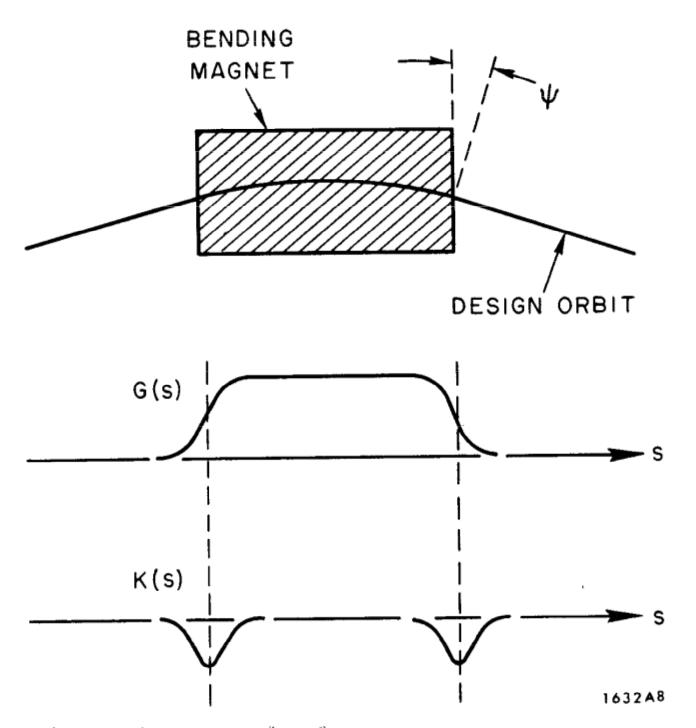
\includegraphics[width=0.6\linewidth]{./Figuras/fig08.jpeg}
	\caption{Guide field with a rectangular magnet.}
	\label{fig:fig8}
\end{figure}

    \section{Equations of motion}\label{sec:2.3}
I would like now to write the equations of motion of an electron that is moving on a trajectory near the design orbit, and with an energy near, but not necessarily at, the design energy. I shall describe the energy of the electron in terms of the deviation $\epsilon$ from the design energy $E_0$:
\begin{align}
	\epsilon = E-E_0
\end{align}
In keeping with our linear approximation I shall keep terms only to first order in the "small” quantities $x$, $y$, and $\epsilon$. Rather than using time as the independent variable it will be more convenient to use the azimuthal coordinate $s$. Derivatives with respect to $s$ will be indicated by the "prime" ('); for example, $x' = dx/ds$.

Let’s begin with the radial motion. Think of an electron that is at $x$ and moving with the slope x’. See Fig.~\ref{fig:fig9}. The slope $x'$ is the angle between the direction of motion of the electron and the tangent to the design orbit. Suppose we call $\theta_0$, the angle between the tangent and some arbitrary reference direction and $\theta$ the angle made by the trajectory with the same reference direction. Then $x' = \tan(\theta - \theta_0) \approx \theta - \theta_0$; and
\begin{align} \label{eq:2.12}
	x'' = \frac{d(\theta-\theta_0)}{ds}.
\end{align}

\begin{figure}[!htb]
	\centering
	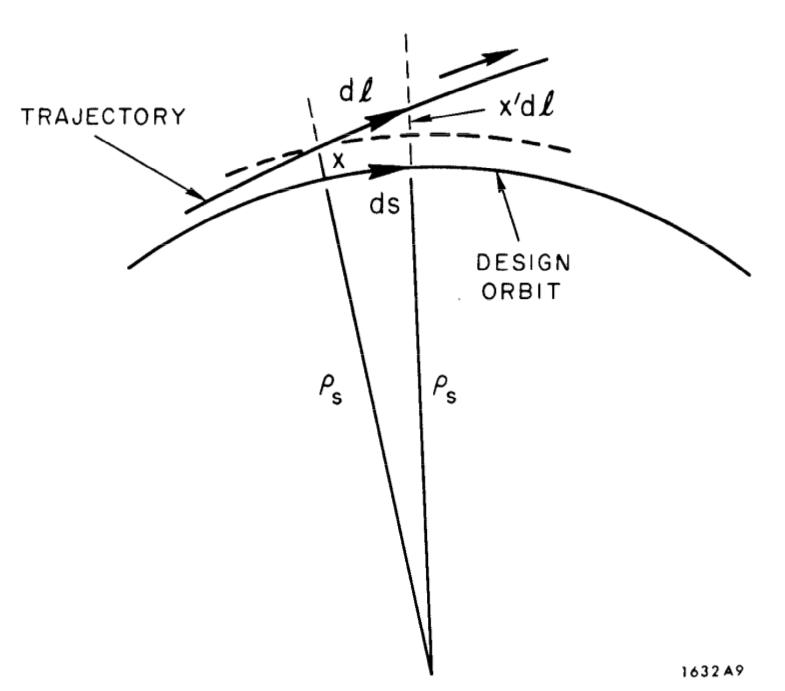
\includegraphics[width=0.6\linewidth]{./Figuras/fig09.jpeg}
	\caption{Electron trajectory near the design orbit.}
	\label{fig:fig9}
\end{figure}

The derivative of $\theta_0$ is, we have seen, just $-1/\varrho_s = -G(s)$. But what is $d\theta/ds$? The radius of curvature of the trajectory is
\begin{align} \label{eq:2.13}
	\varrho = \frac{E}{ecB},
\end{align}
and in a path element $d\ell$ of the trajectory the change in angle is
\begin{align}
	d\theta = -\frac{d\ell}{\varrho} = -\frac{ecB}{E}d\ell\label{eq:2.14}.
\end{align}

Since $\frac{d\ell}{ds} = \frac{d\ell}{d\theta}\frac{d\theta}{d\theta_0}\frac{d\theta_0}{ds}$, then

\begin{align*}
\frac{d\ell}{ds} = \left(-\varrho\right)\frac{d\theta}{d\theta_0}\left(-\frac{1}{\varrho_s}\right).
\end{align*}

Next, notice that so long as the angle $x'$ is small -- as I shall always assume -- the variations of angles $\theta$ and $\theta_0$ are approximately the same in first order,
so $\frac{d\theta}{d\theta_0} \approx 1$. Moreover, the radius of curvature $\varrho$ is $\varrho \approx \varrho_s + x$ in first order again. Thus, a path element $d\ell$ of a trajectory at
$x$ is related to the corresponding change in $s$ by

\begin{align}
	d\ell = \frac{\varrho_s + x}{\varrho_s} ds = \left(1+\frac{x}{\varrho_s}\right)ds = (1+G(s)x)ds\label{eq:2.15}
\end{align}
Next, we may write for $B$
\begin{align}
	B = B_0 + \frac{\partial B}{\partial x}x = \frac{E_0}{ec}(G+K_1x)\label{eq:2.16}
\end{align}
Putting these two into \eqref{eq:2.14} -- together with $E_0 + \epsilon$ for $E$ -- and keeping only first order terms, we find that
\begin{align*}
	d\theta = \left\{-G-(G^2+K_1)x + G\delta\right\}ds
\end{align*}
And so we get from \eqref{eq:2.12} that
\begin{align}\label{eq:2.17}
	x'' = -(G^ 2+K_1)x + G\delta
\end{align}

\begin{proof}
	From \eqref{eq:2.14},
	\begin{align*}
		d\theta &= -\frac{ecB}{E}d\ell\\
				&= -\frac{ecB}{E}(1+Gx)ds\\
				&= -\frac{ec}{E}\left[\frac{E_0}{ec}(G+K_1x)\right](1+Gx)ds\\
				&= -\frac{E_0}{E_0+\epsilon}(G+K_1x)(1+Gx)ds\\
				&= -\frac{E_0}{E_0+\epsilon}(G+(G^2+K_1)x + K_1Gx^2)ds
	\end{align*}

    Keeping only terms to first order,
	\begin{align*}
		d\theta &= \frac{1}{1+\delta}(-G-(G^2+K_1)x)ds
	\end{align*}

	$\delta$ is very small, so we can consider that $\frac{1}{1+\delta}$ is just  the sum of a geometric series. So, we can expand this term in a summatory:
	\begin{align*}
		d\theta &= \left(1 - \delta + \delta^2+ ...\right)(-G-(G^2+K_1)x)ds
	\end{align*}

    Again, keeping only terms to first order,
	\begin{align*}
		d\theta &= \left(1 - \delta\right)(-G-(G^2+K_1)x)ds\\
				&= (-G-(G^2+K_1)x)ds + \left(G\left(\delta\right)+(G^2+K_1)x\left(\delta\right)\right)ds\\
				&= \left\{-G-(G^2+K_1)x + G\delta\right\}ds
	\end{align*}

	Now, from \eqref{eq:2.12},
	\begin{align*}
		x'' &= \frac{d(\theta-\theta_0)}{ds}\\
			&= \left\{-G-(G^2+K_1)x + G\delta\right\} - (-G)\\
			&= -(G^2+K_1)x + G\delta
	\end{align*}
\end{proof}

The corresponding equation for the vertical motion is easier to derive; you can easily see that
\begin{align}
	y'' = K_1 y
\end{align}

\begin{proof}
	For the vertical motion, applying the Lorentz force, we can see that it has the opposite sign from the radial motion:
	\begin{align*}
		d\theta &= -\frac{d\ell}{\varrho} = + \frac{ecB}{E}d\ell\\
				&= \frac{ecB}{E}d\ell\\
				&= \frac{ecB}{E}(1+Gx)ds\\
				&= K_1 y (1+Gx)ds\\
				& = (K_1 y + GK_1xy)ds
	\end{align*}

	Discarding terms to second order,
	\begin{align*}
		d\theta &= K_1 y ds\\
	\end{align*}

	Now, from \eqref{eq:2.12},
	\begin{align*}
		y'' &= \frac{d(\theta-\theta_0)}{ds}\\
			&= \frac{K_1 y\ ds}{ds}\\
			&= K_1 y
	\end{align*}
	keeping in mind that $\frac{d\theta_0}{ds} = 0$ because of our assumption that the design orbit lies in a horizontal plane.
\end{proof}

Notice that with our linearized approximation, the motions in $x$ and $y$ are independent. For our consideration of the electron trajectories, I would like to use the standard form:
\begin{align}
	x'' &= -K_x(s)x + G(s)\delta\label{eq:2.19}\\
	y'' &= -K_y(s)y\label{eq:2.20}
\end{align}
with the definitions:
\begin{align}
	K_x(s) &= G^2(s)+K_1(s) \label{eq:2.21}\\
	K_y(s) &= -K_1(s) \label{eq:2.22}
\end{align}
The term corresponding to $G^2$ is missing from $K_y$ because of our assumption that
the design orbit lies in a plane. Storage rings are most often "strong focusing". For such rings $G^2$ is generally much smaller than $K_1$, so that $K_x$ and $K_y$ are approximately equal and have opposite signs.

The equation for the motion in $y$ looks like the equation of a classical oscillator (force proportional to displacement) with a variable "restoring-force" coefficient -- the function $K_y(s)$. The equation in $x$ is similar except that it has, in addition, a varying "driving term" which is proportional to the energy deviation $\epsilon$. In useful guide fields the solutions are indeed oscillatory, and describe the \textit{lateral oscillations} -- including the so-called \textit{betatron} oscillations -- of the electron trajectories. These oscillations result from the \textit{focusing} properties of the guide field which are characterized by \textit{focusing functions} $K_x$ and $K_y$. As we shall see later, the function $G(s)$ enters as well in the \textit{energy focusing} properties of the guide field.

It is important to remember that all of the focusing functions are necessarily periodic in $s$, the minimum period being one revolution of the ideal orbit; that is, for both $K_x$ and $K_y$ (as well as for $G$)
\begin{align}
	K(s+L) = K(s)\label{eq:2.23}
\end{align}
where $L$ is the length of the ideal orbit. For convenience in construction -- as well as in design -- storage rings generally have also an inner periodicity. That is, they are made up,at least in part, of sequences of identical magnetic \textit{cells},
each cell consisting of a prescribed set of magnets and quadrupoles. Then in a certain span of $s$, the focussing functions will satisfy
\begin{align}
	\left\{\begin{array}{rcl}
	\ G(s+\ell_c) & = & G(s)\\
	K(s+\ell_c) & = & K_1(s)
	\end{array}\right.
\end{align}
where $\ell_c$ is the cell length. Note, however, that while Eq. \eqref{eq:2.23} is true for the \textit{actual} fields of a ring -- since when $s$ is increased by $L$, the electron returns to the same physical point in the ring -- the cell periodicity is a \textit{design} property and will not be strictly true for the actual fields (due to construction imperfections).

It will be useful to have in mind some illustrative example of a guide field. Let’s take the design of the proposed SLAC ring. In it, most of the ring would consist of a repetition of a standard cell, each of which occupies about 1/16 of a full circle. I show in Fig.~\ref{fig:fig10}, the nature of the focusing functions over a part

\begin{figure}[!htb]
	\centering
	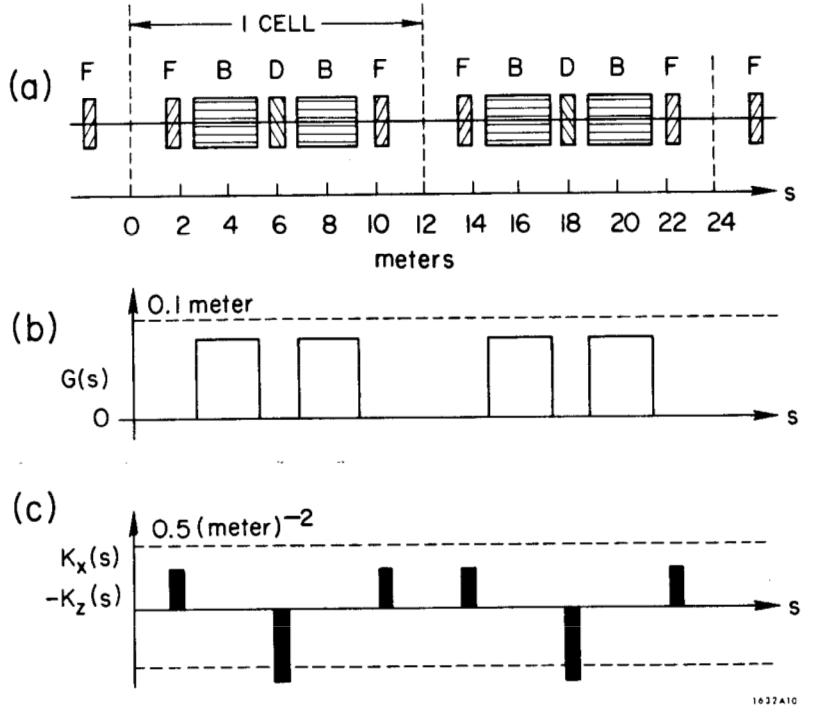
\includegraphics[width=0.7\linewidth]{./Figuras/fig10.jpeg}
	\caption{Magnet lattice and focusing functions in the normal cells
	of a particular guide field.}
	\label{fig:fig10}
\end{figure}
of the ring, comprising two such cells. Part (a) of the figure shows the layout of bending magnets and quadrupoles. The bending magnets designated B, have a uniform field $(dB/dx = 0)$; the quadrupoles have no field on the design orbit $(B_0=0)$ and are designated F or D (for focusing or defocusing in the radial motion) depending on whether their gradients are positive or negative. The other parts of the figure give the focusing functions $G$, $K_x$, and $K_y$.

    \section{Separation of the radial motion} \label{sec:2.4}
It is conceptually convenient to separate the radial motion into two parts, one part being a displaced, closed curve, which is the equilibrium orbit for electrons of the displaced energy, and the other part being the free transverse oscillation about this orbit. Suppose we write for $x$
\begin{align}
	x = x_{\epsilon} + x_{\beta}\label{eq:2.25}
\end{align}
then certainly Eq. \eqref{eq:2.19} is satisfied if both of the following equations are true:
\begin{align}
	x_\epsilon'' &= -K_x(s)x_\epsilon + G(s)\delta\label{eq:2.26}\\
	x_\beta'' &= -K_x(s)x_\beta\label{eq:2.27}
\end{align}
We may make the decomposition unique by requiring that $x_\epsilon(s)$ be a \underline{single-valued function} at each physical azimuth; that is, that $x(s)$ be a function which is periodic in s with period $L$. It is then clear that $x_\epsilon(s)$ is a possible (and in fact, unique) closed orbit for an electron of energy $E_0 + \epsilon$ (with $x_\beta = 0$), and that the general radial motion will consist of the sum of the displacement of this new equilibrium orbit and a \underline{free betatron oscillation} $x_\beta$ which satisfies Eq. \eqref{eq:2.27}.

The displacement $x_\epsilon$ is proportional to the energy deviation $\epsilon$. Let’s write
\begin{align}
	x_\epsilon(s) = \eta(s)\delta\label{eq:2.28}
\end{align}
Now $\eta(s)$ is the single-valued function which satisfies
\begin{align}\label{eq:2.29}
	\begin{cases}
		\eta'' = -K_x(s)\eta + G(s), \\
        \eta(0) = \eta(L), \\
        \eta'(0) = \eta'(L).
    \end{cases}
\end{align}
And the total displacement from the ideal orbit can be written
\begin{align}
	x = \eta(s)\delta + x_\beta
\end{align}
I shall call $\eta(s)$ the off-energy function; it is a unique particular solution of Eq. \eqref{eq:2.29} (because of the required periodicity) and is therefore, a function which characterizes the total guide field. It will be studied in more detail later on.
    \section{Betatron trajectories}\label{sec:2.5}

Equations (2.20) and (2.27) describe the free vertical and radial betatron oscillations. With the approximations made, the motions in the two coordinates are independent. Since the two equations have the same mathematical form -- although the functions $K_y(s)$ and $K_x(s)$ will generally be different -- let’s take as the representative form
\begin{align}
	x'' = -K(s) \; x \label{eq:2.31}
\end{align}
which is the same as Eq. \eqref{eq:2.27} with the subscripts $\beta$ and $x$ suppressed. (With $K(s) = K_x(s)$, Eq. \eqref{eq:2.31} will describe the radial betatron oscillation of an electron of the nominal energy $E_0$; and with $y$ substituted for $x$ and with $K(s) = K_y(s)$, it will describe the vertical motion).

The focussing function $K(s)$ is a prescribed function -- the storage ring design specifies its value at each azimuthal position. If the position and slope ($x$ and $x'$) of an electron are given for some azimuth, the subsequent motion is uniquely determined. It can in fact be determined by a direct numerical integration of Eq. \eqref{eq:2.31}. Generally, however, the guide field is constructed of magnetic segments, in each of which $K(s)$ may be taken as a constant so that the integration can be made algebraically for each segment and the motion can be pieced together from such solutions. Depending on whether the value of K is positive, zero, or negative in a particular segment of $s$, the motion in $x$ will have one of the forms
\begin{align}
	\left\{\begin{array}{l}
	K>0: \ \ x = a\ \cos(\sqrt{K}s+b) \\
	K=0: \ \ x = as+b \\
	K<0: \ \ x = a\ \cosh(\sqrt{-K}s+b)
	\end{array}\right. \label{eq:2.32}
\end{align}
where $a$ and $b$ are constants in each segment -- and may be determined from the values of $x$ and $x'$ at the entrance to the segment (since $K$ is everywhere finite, $x$ and $x'$ must both be everywhere continuous -- and,in particular, at the boundary between the two segments).

As an illustration suppose we consider the motion for a $K(s)$ like that shown for $K_x(s)$ in Fig.~\ref{fig:fig10}. Two possible trajectories are shown in (b) of Fig.~\ref{fig:fig11}. The first one is a trajectory which starts at $s_0$ with a unit displacement ($x_0 = 1$) but no slope ($x_0' = 0$); and the second starts at $s_0$ with zero displacement but with a unit slope ($x_0' = 1$). Each of them is made up of pieces described by one of the functions in \eqref{eq:2.32}. There are, of course, an infinite number of possible trajectories, depending on the initial conditions at $s_0$; but the two shown are of particular interest. The first one is called (for \textit{any} chosen $s_0$) the “cosine-like” trajectory associated with so and is designated $C(s,s_0)$; the other one is the “sine-like” trajectory $S(s,s_0)$.

\begin{figure}[!htb]
	\centering
	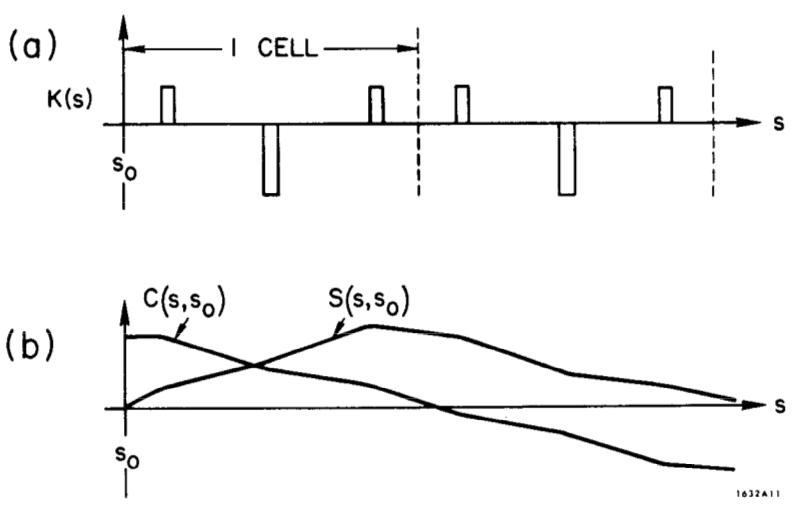
\includegraphics[width=0.7\linewidth]{./Figuras/fig11.jpeg}
	\caption{Focussing function $K(s)$ and two trajectories: the cosine-like trajectory and the sine-like trajectory for the starting azimuth $s_0$.}
	\label{fig:fig11}
\end{figure}

The detailed form of $C$ and of $S$ will depend on the reference azimuth $s_0$. They are in general, \textit{not} periodic functions, even though $K(s)$ is. For a ring with stable trajectories, $C$ and $S$ are bounded oscillatory functions which have a different shape on each successive revolution of the ring; although they are "quasi-periodic” in the sense that after some number of revolutions they will lie very close (or in some hypothetical cases even exactly on) the trajectory of an earlier revolution.

Now since Eq.~\eqref{eq:2.31} is linear in $x$, any linear combination of $C$ and $S$ will also describe a possible trajectory; and more particularly, all possible trajectories can be described by such a linear combination. That is, for any trajectory
\begin{align}
	x(s) &= C(s,s_0)x_0 + S(s,s_0)x_0'\\
	x'(s) &= C'(s,s_0)x_0 + S'(s,s_0)x_0'
\end{align}
where $C'$ and $S'$ are the derivations of $C$ and $S$ with respect to $s$; and $x_0$ and $x_0'$ are the values of $x$ and $x_0'$ at $s_0$.

It is often convenient to write the last two equations in a matrix notation. Let's let $\boldsymbol{x}(s)$ stand for the “vector” whose components are $x(s)$ and $x'(s)$;
\begin{align}
	\boldsymbol{x}(s) = \begin{bmatrix}
	x(s)\\ 
	x'(s)
	\end{bmatrix}
\end{align}
Then we may write that
\begin{align}
	\boldsymbol{x}(s)=\boldsymbol{M}(s,s_0)\boldsymbol{x}(s_0)
\end{align}
in which $\boldsymbol{M}$ is the transfer matrix to $s$ from $s_0$, which depends only on the properties of the guide field between the two azimuths. It's elements can be written in terms of the cosine-like and sine-like functions:
\begin{align}
	\boldsymbol{M}(s,s_0) = \begin{bmatrix}
	C(s,s_0) & S(s,s_0)\\
	C'(s,s_0) & S'(s,s_0)
	\end{bmatrix}\label{eq:2.37}
\end{align}
The transfer matrix for any span of $s$ can often be conveniently found in terms ofthe matrices for segments of the span, since for any $s_1$ between $s_0$ and $s$,
\begin{align}
	\boldsymbol{M}(s,s_0) = \boldsymbol{M}(s,s_1)\boldsymbol{M}(s_1,s_0)
\end{align}
The matrix for a segment which extends from $s_1$ to $s_2 = s_1 + \ell$ with a constant $K$ is given in Table~\ref{tab:tab1} for the three cases; $K > 0$, $K = 0$, and $K < 0$. They may be derived from the equations in \eqref{eq:2.32}.

The transfer matrix method is useful when designing a ring, or in looking at special problems such as the initial trajectories at injection. It does not, however, provide the most convenient description of the general nature of the trajectories of stored electrons. For many purposes another method of describing the trajectories is more useful. It may be called the "pseudo-harmonic" description.
\begin{table}[!ht]
	\caption{Transfer matrices for segments of constant $K$.}
	\centering
	\begin{tabular}{lrl}
		$K>0:$ & $\boldsymbol{M}(s_2,s_1) =$ &  $\begin{bmatrix}
			\cos(\sqrt{K}\ell) & \frac{1}{\sqrt{K}}\sin(\sqrt{K}\ell)\\
			-\sqrt{K}\sin(\sqrt{K}\ell) & \cos(\sqrt{K}\ell)
			\end{bmatrix}$\\
		\\
		$K=0$: & $\boldsymbol{M}(s_2,s_1) =$ & $\begin{bmatrix}
			1 & \ell\\
			0 & 1
			\end{bmatrix}$\\
		\\
		$K<0:$ & $\boldsymbol{M}(s_2,s_1) =$ & $\begin{bmatrix}
				\cosh(\sqrt{-K}\ell) & \frac{1}{\sqrt{-K}}\sinh(\sqrt{-K}\ell)\\
				\sqrt{-K}\sinh(\sqrt{-K}\ell) & \cosh(\sqrt{-K}\ell)
				\end{bmatrix}$
	\end{tabular}
	\label{tab:tab1}
\end{table}

The general solutions of Eq.~\eqref{eq:2.31} can be written as
\begin{align}
	x(s) = a\zeta(s)\ \cos\{\varphi(s)-\vartheta\}\label{eq:2.39}
\end{align}
where $\zeta(s)$ and $\varphi(s)$ are specially defined functions of $s$ with certain convenient properties and $a$ and $\vartheta$ are constants ("initial conditions") which determine a particular trajectory. Specifically, if we define
\begin{align}
	\varphi(s) = \int_{0}^{s} \frac{d\bar{s}}{\zeta^2(\bar{s})}
\end{align}
so that
\begin{align}
	\varphi'(s) = \frac{1}{\zeta^2}
\end{align}
and if we define $\zeta(s)$ to be that positive valued, analytic function which satisfies
\begin{align}
	\zeta'' = -K(s)\zeta+\frac{1}{\zeta^3}\label{eq:2.42}
\end{align}
then, as you can show by direct substitution, the $x(s)$ of Eq.~\eqref{eq:2.39} satisfies the differential equation~\eqref{eq:2.31}. For a more rigorous approach, you can check the appendix, Section~\ref{sec:FloquetTheorem}.

Following tradition, I shall choose generally to deal rather than with $\zeta(s)$, with its square -- which is universally written as $\beta(s)$. With this translation Eq.~\eqref{eq:2.39} gets replaced by
\begin{align}
	x(s) = a\sqrt{\beta(s)}\ \cos\{\varphi(s)-\vartheta\}\label{eq:2.43}
\end{align}
with
\begin{align}
	\varphi(s) = \int_{0}^{s} \frac{d\bar{s}}{\beta(\bar{s})}\label{eq:2.44}
\end{align}
and
\begin{align}
	\beta(s) = \zeta^2(s)\label{eq:2.45}
\end{align}
so that $\sqrt{\beta(s)}$ is the function defined by Eq.~\eqref{eq:2.42}. Given the focusing function $K(s)$ for a storage ring, the function $\beta(s)$ is uniquely determined; it can therefore, serve as an alternate “representation” of the focusing characteristics of the ring. Notice, however, that while $K(s)$ is given in terms of the local properties (at each $s$) of the guide field, the function
$\beta(s)$ -- or $\zeta(s)$ -- depends on the total configuration of the ring. On the other hand once $\beta(s)$ is known, $K(s)$ can be immediately obtained from its local derivatives by Eqs. \eqref{eq:2.42} and \eqref{eq:2.45}. But it is $\beta(s)$ which reveals more directly the significant characteristics of the trajectories of stored electrons.

It is possible to have guide fields that do not result in stable (that is, bounded) trajectories. For such fields $\beta(s)$ is not defined. But such fields can hardly be said to form a "storage" ring; so we are not interested in them here. Although they may be of interest to the storage ring designer -- as something to be avoided!

I will return later to a discussion of how $\beta(s)$ is related to the guide field properties; but it will be more useful to look first at the qualities of the trajectories described by the pseudo-harmonic solutions described by Eq.~\ref{eq:2.43}. 

Don't forget that all of the discussion of this section applies equally to vertical as well as to radial motion. A ring is therefore, described by the two functions $\beta_x$ and $\beta_y$ (or $\zeta_x$ and $\zeta_y$), which are derived from the two focussing functions $K_x$ and $K_y$. It follows that the phase function $\varphi(s)$ is also different for motion in $x$ and in $y$.

    \section{Pseudoharmonic betatron oscillations}\label{sec:2.6}
We have seen that the betatron oscillations -- in either $x$ or $y$ -- are described by a pseudo-harmonic oscillation whose representative form is
\begin{align}
	x(s) &= a\sqrt{\beta}\ \cos\{\varphi-\vartheta\}\label{eq:2.46}\\
	\varphi &= \int_{0}^{s} \frac{d\bar{s}}{\beta}\label{eq:2.47}
\end{align}
where $\beta$ is a given function of $s$, which we may call the betatron function, and $a$
and $\vartheta$ are constants of the particular trajectory. The two equations above describe completely the path taken by the electron. To get a complete picture of the motion of the electron in the coordinate $x$ we must only add the fact that the electron travels always at the speed $c$ of light. For many purposes it is adequate to take that the azimuth of the electron varies simply as
\begin{align}
	s = s_0 + ct\label{eq:2.48}
\end{align}
You should remember, however, that this is only an approximation which neglects terms that are the order of $x/\varrho_s$, where $\varrho_s$, is the radius of curvature of the design orbit. The correction terms to Eq.~\eqref{eq:2.48} will be looked at in Section~\ref{sec:3.2}.

The betatron function describes completely the lateral focussing properties of the guide field. By its nature the betatron function must be always positive-definite; it has a “wave-like” character, and in a well-designed ring it will wander not too far (say a fraction of an order-of-magnitude) from its mean value. It might typically look like the curve (a) in Fig.~\ref{fig:fig12}. The definition of $\beta(s)$ constrains it to be periodic in $s$ with the period $L$:
\begin{align}
	\beta(s+L) = \beta(s)
\end{align}
It has a unique value at each physical azimuth. If the guide field has a higher rotational symmetry -- being composed of two or more identical periods -- $\beta$ will have the same symmetry. A guide field which produces the $\beta$ of Fig.~\ref{fig:fig10}(a) would have sixteen identical cells in its circumference. Note, however, that a local periodicity in the focussing functions $G(s)$ and $K(s)$ in only a part of the guide field will not, in general, give rise to a corresponding local periodicity in $\beta$. It will do so only when the local periodicity is repeated all the way around the ring to produce a true rotational symmetry.

As the electron travels around the ring it executes a lateral oscillation which is not harmonic -- nor periodic. The motion is a kind of distorted sine-wave with a varying amplitude ($a\sqrt{\beta}$) which is modulated in proportion to the root of the betatron function, and with a “phase” ($\varphi-\vartheta$) which advances with $s$ at a varying rate proportional to $1/\beta$. The nature of the motion is illustrated in parts (b) and (c) of Fig.~\ref{fig:fig12}. The two segments of trajectory shown correspond to the same 2, but to different starting phases.

Suppose that we chose some initial $a$ and $\vartheta$, and follow the trajectory for many successive revolutions. We would get a path such as the one shown in part (d) of Fig.~\ref{fig:fig12}, where, for convenience, I have superimposed all of the successive revolutions on the same segment of $s$. (Or, if you wish, since $s$ is a cyclic variable, I am plotting $s$ (modulo $L$) instead of $s$). The picture gives some idea of what we would see if we watched a single stored electron circulating in a ring.

\begin{figure}[!htb]
	\centering
	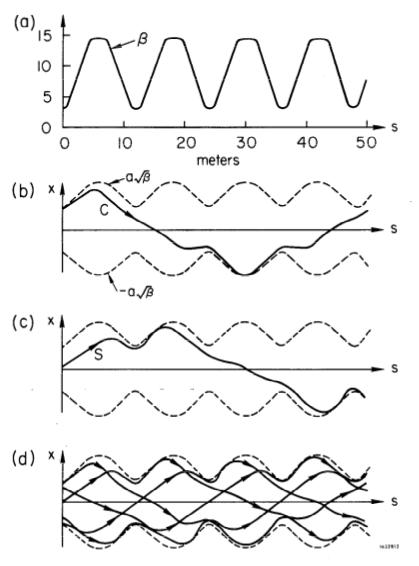
\includegraphics[width=0.7\linewidth]{./Figuras/fig12.jpeg}
	\caption{a) Betatron function. (b) Cosine-like trajectory for $s=O$. (c) Sine-like trajectory for $s=O$. (d) One trajectory on several successive revolutions.}
	\label{fig:fig12}
\end{figure}

One important feature of the betatron motion is evident in Fig.~\ref{fig:fig12}(d) -- at each physical azimuth the displacement $x$ of a circulating electron lies always below a limiting extreme value $X(s)$ obtained by setting $cos(\varphi - \vartheta) = 1$; namely
\begin{align}
	X(s) = a\sqrt{\beta(s)}
\end{align}
The complete trajectory of a stored electron will fall forever within an envelope defined by $\pm X(s)$. And it follows that the aperture required to contain an electron with a given oscillation amplitude varies around the ring as $X(s)$. The ratio of the envelope width at two locations $s_1$ and $s_2$ is, of course, just
\begin{align}
	\frac{X_2}{X_1} = \sqrt{\frac{\beta_2}{\beta_1}}
\end{align}
At each physical azimuth a stored electron may generally be expected to pass frequently with a displacement near the maximum.

Let's look now at the slope of the betatron trajectory, $x' = dx/ds$. Taking the derivative of Eq.~\eqref{eq:2.46}, we may write
\begin{align}
	x' = - \frac{a}{\sqrt{\beta}}\sin(\varphi-\vartheta)+\frac{\beta'}{2\beta}x\label{eq:2.52}
\end{align}
The first term comes from the changing phase; and the second from the variation of $\beta$.

Notice that the zeros of $x'$ -- and therefore, the peak values of $x$ -- do not occur when $cos(\varphi - \vartheta)$ is 1. Rather they are reached when
\begin{align}
	\tan(\varphi-\vartheta) = \frac{\beta'}{2}
\end{align}
which means that
\begin{align}
	\cos(\varphi-\vartheta) = \left[1+\frac{\beta'^2}{4}\right]^{-\frac{1}{2}}
\end{align}
If the peak of a particular cycle of an oscillation occurs at some $s$, the peak displacement then will be
\begin{align}
	x_{peak} = a\sqrt{\beta}\left[1+\frac{\beta'^2}{4}\right]^{-\frac{1}{2}}
\end{align}
See Fig.~\ref{fig:fig13}

\begin{figure}[!htb]
	\centering
	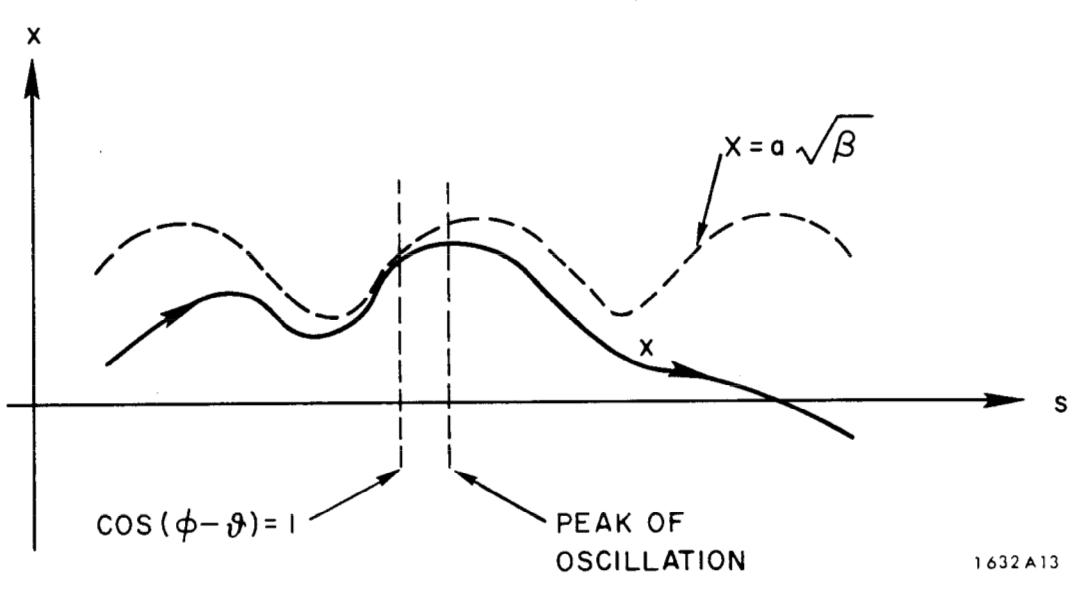
\includegraphics[width=0.8\linewidth]{./Figuras/fig13.jpeg}
	\caption{The maximum of a particular cycle of a betatron oscillation.}
	\label{fig:fig13}
\end{figure}

In a classical harmonic oscillation the amplitude is an invariant of the motion. Its square is proportional to the energy of the oscillator, and can be expressed as a quadratic function of the instantaneous position and velocity. The corresponding invariant of the pseudo-harmonic oscillator is the constant $a$.

If we isolate the cosine and sine terms in Eqs. \eqref{eq:2.46} and \eqref{eq:2.52}, square them, and add, we can relate $a^2$ to $x$ and $x'$. We find that
\begin{align}
	a^2 = \frac{x^2}{\beta} + \beta\left[x'-\frac{\beta'}{2\beta}x\right]^2\label{eq:2.56}
\end{align}
If we know $x$ and $x'$ at any azimuth, say $s_1$, $a$ can be found and all subsequent displacements can be expressed by
\begin{align}
	x = \frac{1}{\sqrt{\beta_1}}\left[x_1^2+\left(\beta_1x'_1-\frac{x_1\beta'_1}{2}\right)^2\right]^\frac{1}{2}\sqrt{\beta}\ \cos(\varphi-\vartheta)\label{eq:2.57}
\end{align}
The phase constant $\vartheta$ must also be determined from $x$ and $x'$. It can be obtained from
\begin{align}
	\tan(\varphi_1 - \vartheta) = -\frac{\beta_1 x'_1}{x_1}+\frac{\beta'_1}{2}
\end{align}
where $\varphi_1 = \varphi(s_1)$.

We are often interested only in the maximum value $X(s)$ which can be reached at any physical azimuth on any subsequent revolution. This maximum is independent of $\vartheta$ and is obtained by replacing the cosine factor of Eq.~\eqref{eq:2.57} by 1:
\begin{align}
	X(s) = \frac{1}{\sqrt{\beta_1}}\left[x_1^2+\left(\beta_1x'_1-\frac{x_1\beta'_1}{2}\right)^2\right]^\frac{1}{2}\sqrt{\beta(s)}
\end{align}

If $\beta$ were everywhere comparable -- say not too far from some typical value $\beta_n$ then the ensuing peak amplitude which would result from a sudden lateral displacement $\delta x$ would be about equal to $\delta x$, and the amplitude which would result from a sudden lateral impulse that changed the slope by $\delta x'$ would be about proportional to $\beta_n \delta x'$. Generally, we may expect that the amplitudes which result from disturbances to the trajectory will be less the smaller is $\beta$. Indeed, we may consider that $1/\beta$ is a measure of the “strength” of the lateral focusing, and that small values of $\beta$ are generally desirable.

    \section{The tune} \label{sec:2.7}

As an electron makes one complete revolution of a storage ring starting at some azimuth, say $s_0$, its oscillation phase $(\varphi - \vartheta)$ advances by
\begin{align*}
	\int_{s_0}^{s_0+L}\dfrac{ds}{\beta}.
\end{align*}
Because of the periodicity of $\beta$ this integral is the same for all $s_0$: in any complete revolution the phase increases by the same amount. This phase advance is an important parameter of a storage ring and is usually written as $2\pi\nu$ (although in Europe we have the definition often $2\pi Q$); and $\nu$ is called the tune. We have the definition

\begin{align}\label{eq:2.60}
	\boxed{\nu = \dfrac{1}{2\pi} \int_s^{s+L} \dfrac{d\bar{s}}{\beta} = \dfrac{1}{2\pi}\int_0^L \dfrac{d\bar{s}}{\beta} = \dfrac{1}{2\pi} \oint \dfrac{ds}{\beta}}.
\end{align}

(I shall use from now on the complete integral symbol $\oint$ to indicate any integral
around the whole ring.) The tune for the two oscillation coordinates
$x$ and $y$ - written as $\nu_x$ and $\nu_y$ - are generally different, being derived from the two betatron functions $\beta_x$ and $\beta_y$. Both $\nu_x$ and $\nu_y$ are typically not-too-large numbers near, but not at a quarter integer- such as 2.78 or 5.15. Other ways of calculating $\nu$ will be treated in Section \ref{sec:2.10}.

Although the betatron trajectory is a contorted aperiodic oscillation, if we sit at some particular azimuth and observe the successive passages of a stored electron we find that the displacement follow a simple sinusoidal law. Suppose we pick our observation point at $s_0$, and let the successive passages past this azimuth be identified by the index $j=0,1,2,3,...$ Also let $\varphi_0$ be the phase at the zero-th passage. On each successive passage the phase will increase by $2\pi \nu$; at the $j$-th passage the phase will be
\begin{align*}
	2\pi \nu j + \varphi_0.
\end{align*}
and the displacement will be
\begin{align}\label{eq_xj}
	x_j = a \sqrt{\beta_0} \cos(2\pi \nu j + \varphi_0).
\end{align}
The “amplitude” factor $(a \sqrt{\beta_0})$ is a constant ($\beta_0 = \beta(s_0)$), so the displacement, as sampled each revolution, varies as the sampling of a simple sinusoidal oscillation.

Since the time for each revolution is constant\footnote{Neglecting a small correction proportional to $x$.}, namely $L/c$, we may also write that the time $t_j$ of the $j$-th passage is
\begin{align*}
	t_j = \dfrac{L}{c}j;
\end{align*}
or that
\begin{align}
	2\pi j = \omega_r t_j,
\end{align}
where
\begin{align}
	\omega_r = 2\pi \dfrac{c}{L},
\end{align}
is the (angular) frequency of revolution of the electron. Then \eqref{eq_xj} becomes, for any fixed $s$,
\begin{align}
	x_s(t_j) = a \sqrt{\beta(s)}\cos(\nu \omega_r t_j + \varphi_{0s}).
\end{align}
When observed at a particular azimuth the lateral motion is indistinguishable from a sampled simple harmonic oscillation  at the frequency $\nu \omega_r$ - generally called the betatron frequency.

Looking at Eq. \eqref{eq_xj} we can see the justification for the statement of the preceding section that at each azimuth we may sooner-or-later expect to see $x$ take on its maximum value $X(s)=a\sqrt{\beta(s)}$. Unless $\nu$ is an integer, or better,unless the difference between $\nu$ and an integer is a simple fraction - which is not likely to be exactly true for a real storage ring - the phase (modulo $2\pi$) at successive passages of any fixed point will "walk" through a large number of values between $0$ and $2\pi$ before repeating itself. And the displacement will sooner-or-later take on its peak value $X$ at, or near, each azimuth.

Perhaps the most important significance of the tune $\nu$ of a storage ring is related to the existence of disturbing \textit{resonances} which appear if $\nu$ takes on certain values. For example, if $\nu$ were an integer, the betatron oscillation would ideally become quite periodic repeating itself each revolution. However, the smallest imperfection in the guide field (and there will surely be at least one!) will act as a perturbation which is synchronous with the oscillation frequency. A synchronous perturbation leads to a resonance excitation of the oscillations and an exponential growth of the amplitude.  There will be no stable oscillation (Said in another way, the betatron function of the actual machine may not be defined.) As we shall see later, other resonances will occur also at half-integral values of $\nu$; or if nonlinear effects are taken into account when the difference between $\nu$ and an integer is any simple fraction.

Resonances must, of course, be avoided in both the radial and vertical betatron oscillations. It turns out that resonances of some kind may occur when $\nu_x$ and $\nu_y$ satisfy
\begin{align}\label{eq_ressonance_relation}
	m \nu_x + n \nu_y = r, 
\end{align}
where $m$, $n$, and $r$ are integers. Significant effects are  Significant effects are generally observed only for low-order resonances, that is, those for which $m$, $n$, $r$ take on the small values $0, 1, 2, 3$. The operating point of a storage ring is specified by giving both $\nu_x$
and $\nu_y$ and must be chosen to avoid the serious resonances. The resonance relation \eqref{eq_ressonance_relation} defines a set of lines in a $(\nu_x, \nu_y)$ diagram. Some of them are shown in Fig. \ref{fig:lower_order_resonance_lines}, where a possible operating point is also indicated. For one particular set of resonances, namely when $\nu_x$ is equal to $\nu_y$ or when their difference is integer,there will be strong coupling between the horizontal and vertical oscillations. At such a resonance our assumption of completely independent oscillations is no longer valid and the motion will be more complicated. Sometimes a storage ring may intentionally be operated on or near such a coupling resonance in order to increase the amplitude of vertical oscillations by feeding them energy from the radial oscillation. \\
To stay clear of dangerous resonances it is necessary that the actual operating point remain fairly close to the chosen one - as is clear from Fig. \ref{fig:lower_order_resonance_lines}. We may expect that magnet imperfections will generally cause shifts of $\nu$ which are proportional to $\nu$ itself. A storage ring with a large tune is likely to be a “touchy” machine. This is one of the reasons that designers tend to choose $\nu$ values between about 2 and 6.

\begin{figure}[!htb]
	\centering
	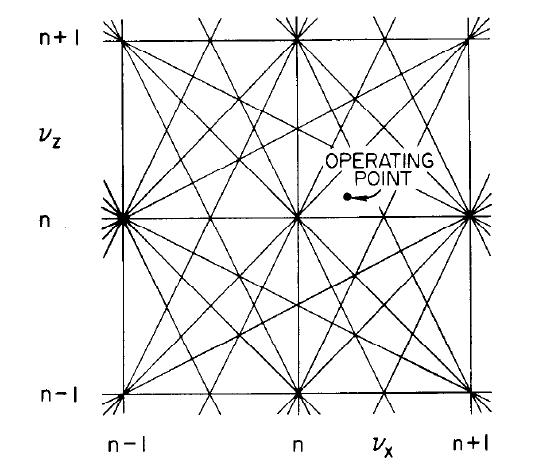
\includegraphics[width=0.7\linewidth]{./Figuras/fig14.jpeg}
	\caption{Lower-order resonance lines on a $\nu_x$, $\nu_y$ diagram.}
	\label{fig:lower_order_resonance_lines}
\end{figure}

    \section{Action Angle Variables} \label{sec:2.8}


    \section{Nature of the betatron function}\label{sec:2.9}

The storage-ring designer is very much occupied with finding a magnet design which will provide a suitable betatron function $\beta(s)$. And a user may generally expect that along with the design of the ring will come a plot of that function.  I do not wish here to go into the intricate matter
 of the techniques for arriving at a design which will yield a "good" $\beta(s)$, but rather I would like only to give some idea about how $\beta(s)$ may be evaluated for a given set of magnet parameters. \\
What is a desirable form for $\beta(s)$? We have already seen at the end of Section \ref{sec:2.7} that at least in certain respects, small values of $\beta$ (strong focusing) are desirable - provided that $\beta$ is reasonably uniform. Unfortunately, small $\beta$’s can only be obtained with alternating gradient focusing which tends to give reasonably large undulations to $\beta$. Also, smaller $\beta$’s imply larger values of $\nu$, which may, as remarked in Section \ref{sec:2.7}, lead to greater difficulties from resonances. \\
In Section \ref{sec:2.6} the betatron function $\beta(s)$ was defined as that single-valued continuous function whose square root $\zeta(s)$ satisfies
\begin{align} \label{eq:2.74}
	\zeta''+K(s)\zeta-\dfrac{1}{\zeta^3}=0
\end{align}
where $K(s)$ is the magnet focusing function. The typical modern storage ring is made up of a chain of segments in each of which the function $K(s)$ has a constant value, positive, negative,
 or zero. An example was given in Fig. \ref{fig:fig11}(a), with the corresponding $\beta=\zeta^2$ shown in Fig. \ref{fig:fig12}(a).
The requirement that $\zeta(s)$ be periodic, together with the nonlinear term $1/\zeta^3$, gives a unique specification - including the scale. The function $\zeta(s)$ is the “eigenfunction” of Eq. \eqref{eq:2.74} and because of the non-linearity, there is no arbitrary normalization of the amplitude. \\
From a dimensional argument we would expect that $\zeta$ should scale as $|K|^{-1/4}$, or that $\beta$ should scale $|K|^{-1/2}$. (Recalling that $1/\beta$ is like the "frequency" of an
oscillator we might expect it to go as the root of the “restoring force constant”.) For a given geometry of the field, such a scaling law is roughly true. \\
In a region of $s$ where $K(s)$ is a constant Eq. \eqref{eq:2.74} has just the form of the
one-dimensional equation of motion of a particle being acted on by a linear “restoring” force $-K\zeta$ and a “repulsive core” force $1/\zeta^3$. Or if you prefer, of a particle which moves with a potential energy proportional to
\begin{align*}
	K \zeta^2 + \dfrac{1}{\zeta^2}.
\end{align*}
(The second term is much like a “centrifugal barrier”!) The shape of the effective potential is shown in Fig. \ref{fig:fig16} for $K > 0$, $K = 0$, and $K < 0$. In any region where $K \leq 0$ the acceleration in $\zeta$ (the displacement of the model particle) is always positive; and $\zeta$ is driven always toward larger values - or, of course, turned around
if it has an initial velocity toward the origin of $\zeta$. For negative $K$ the driving force
is, at large $\zeta$, proportional to the size of $K$. On the other hand, in any region
where $K > 0$ there will be a nice stable potential well, and when $\zeta$ is large, there
is always a “force” driving it toward the origin.

\begin{figure}[!htb]
	\centering
	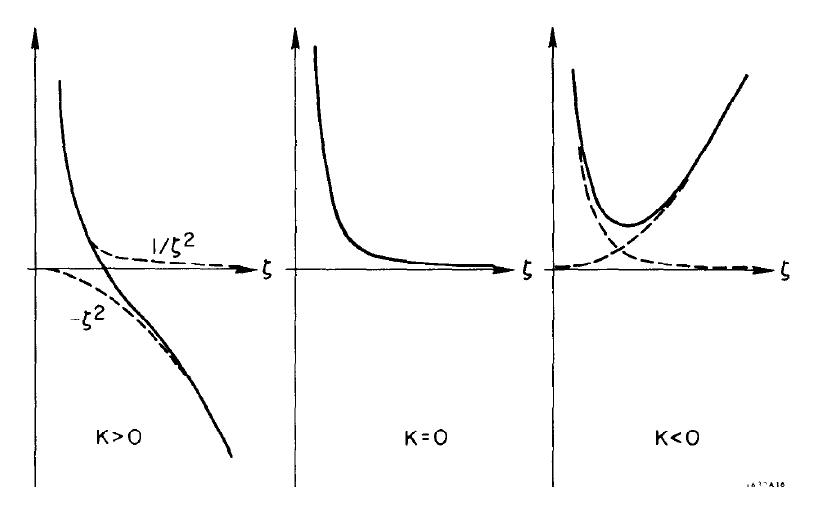
\includegraphics[width=0.8\linewidth]{./Figuras/fig16.jpeg}
	\caption{Effective "potential" functions for $\zeta$.}
	\label{fig:fig16}
\end{figure}

It is also qualitatively apparent that there may exist "stable''  solutions for which $\zeta(s)$ enters a region of $K > 0$ moving inward (toward the origin) and is turned around by the "repulsion" only to be sent back inward again by the "attractive" force in a later region where $K < 0$. For a periodic $K(s)$ like that in Fig. \ref{fig:fig17}, we must expect a solution $\zeta(s)$ like the one sketched in part (b). The solution exhibits an important general characteristic of the function $\zeta(s)$: its maxima occur in focusing sections - one where $K > 0$ - and its minima occur in defocusing sections - where $K < 0$.

\begin{figure}[!htb]
	\centering
	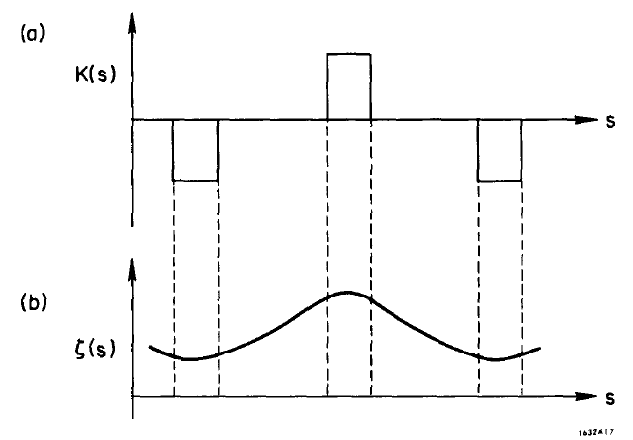
\includegraphics[width=0.8\linewidth]{./Figuras/fig17.jpeg}
	\caption{Form of the function $\zeta(s)$ with a periodic focusing function $K(s)$.}
	\label{fig:fig17}
\end{figure}

It is also clear that, for a given spacing of the segments of different $K$-values, if the magnitude of $K$ is scaled upward, the amplitude of the undulations will grow rapidly larger. Less apparent - and left as a point to ponder - is the fact that as the scale of $K$ is increased a situation will be eventually reached for which a "stable" - i.e., periodic - solution no longer exists for $\zeta(s)$. So the strength of the focusing (magnitude of $K$) and the element spacing must be adjusted together in playing with a storage ring \emph{lattice} (a word used to indicate the geometry of the segments).

You may be tempted to wonder: "Why not just have $K > 0$ at all $s$? Clearly the stability of $\zeta(s)$ is then guaranteed". But do not forget that when $K$ is positive for one coordinate
 of lateral motion in the storage ring - say $x$ - then the $K$ for the other coordinate - $y$ - is negative, and vice-versa. Recall Eqs. \eqref{eq:2.21} and \eqref{eq:2.22}. The need for an alternating gradient is clear.\\
It should also be now apparent that the undulations of $\zeta(s)$ - and so also of $\beta(s)$ - will be “out-of-phase” in the two coordinates $x$ and $y$, the $\zeta$ for one being at
its maximum where the $\zeta$ for the other is at its minimum.\\
The out-of-phase behavior is quite general - even for rather complicated focusing lattices - although it will not generally be true that the $\zeta_x(s)$ and $\zeta_y(s)$ are entirely
 similar in shape. In Fig. \ref{fig:fig18} I show the two functions $\zeta_x$ and $\zeta_y$ for the periodic lattice of Fig. \ref{fig:fig10}.

\begin{figure}[!htb]
	\centering
	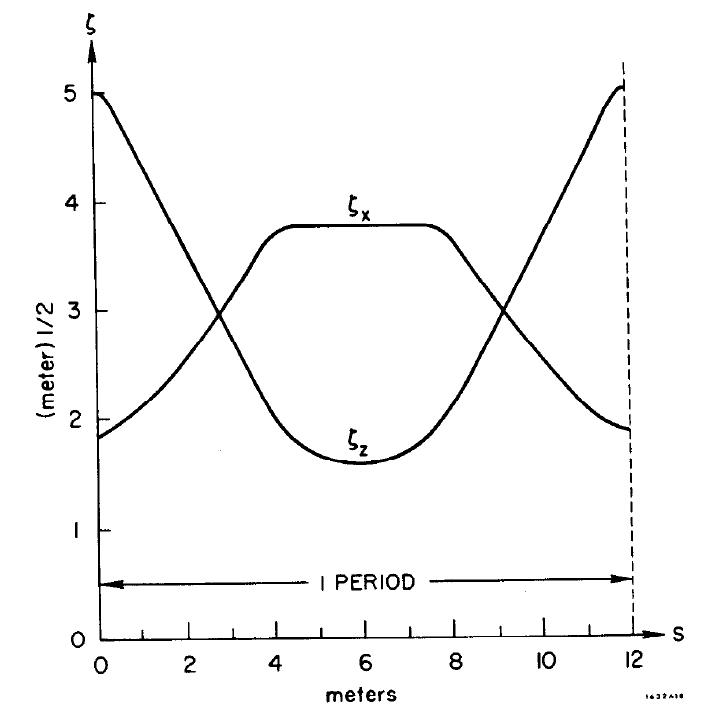
\includegraphics[width=0.8\linewidth]{./Figuras/fig18.jpeg}
	\caption{The functions $\zeta_x$ and $\zeta_y$, for the guide field of Fig. \ref{fig:fig10}.}
	\label{fig:fig18}
\end{figure}

It is instructive to relate the betatron function $\beta(s)$ to the sine-like trajectories which were defined in Section \ref{sec:2.6}. The sine-like trajectory $S(s, so)$ associated with the azimuth $s_0$ is that trajectory which starts at so with zero displacement
and unit slope. It can be expressed in terms of the pseudo-harmonic oscillation Eq. \eqref{eq:2.46} by setting $a = \sqrt{\beta(s_0)}$ and $\vartheta = \pi/2+\varphi(s_0)$:
\begin{align}
	S(s,s_0) = \sqrt{\beta(s_0)\beta(s)}\sin\int_{s_0}^s\dfrac{d\bar{s}}{\beta(\bar{s})}.
\end{align}
(You can check that $S(s_0, s_0) = 0$, and $S'(s_0, s_0) = 1$.) Now consider what happens if we follow this sine-like trajectory for one complete revolution - that is to $s = s_0 + L$. The integral becomes, by Eq. \eqref{eq:2.60} just $2\pi\nu$. Because of the periodicity of the betatron function, $\beta(s_0 + L) = \beta(s_0)$. So
\begin{align}
	S(s_0+L,s_0)=\beta(s_0)\sin2\pi\nu
\end{align}
which - since $\nu$ is independent of $s_0$ - I can also write as

\begin{align}\label{eq:2.77}
	\beta(s)=\dfrac{S(s+L,s)}{\sin2\pi\nu}.
\end{align}
The betatron-function at $s$ is, within a constant, just the displacement after one revolution
 of the sine-like trajectory which starts at $s$. See Fig. \ref{fig:fig19}.\\
We now have another prescription for finding $\beta(s)$. One needs only calculate directly the sine-like trajectory after one revolution, starting at each $s$.\\
\begin{figure}[!htb]
	\centering
	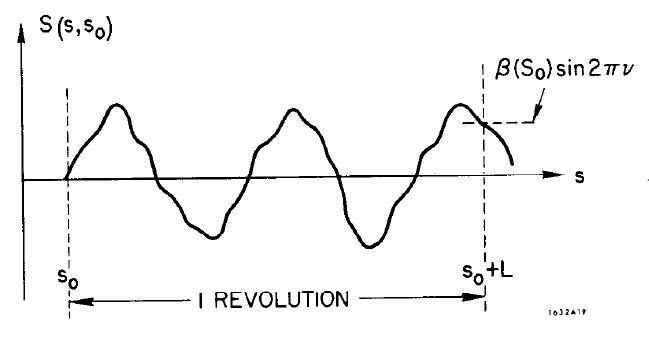
\includegraphics[width=0.8\linewidth]{./Figuras/fig19.jpeg}
	\caption{Relation between $S(s, s_0)$ and $\beta(s_0)$.}
	\label{fig:fig19}
\end{figure}
The displacements obtained are proportional to $\beta(s)$. There is left only to determine the "normalization" factor $1/2\pi\nu$. Using the definition of $\nu$, Eq. \eqref{eq:2.60} together with Eq. \eqref{eq:2.77}, you can see that $\nu$ can be obtained as the solution of the transcendental equation
\begin{align}
	\dfrac{2\pi\nu}{\sin{2\pi\nu}}=\oint\dfrac{ds}{S(s+L,s)}.
\end{align}
So, given $S(s+L, s)$ for all $s$, we can determine uniquely $\beta(s)$.\\
The calculation of $S(s +L, s)$ can be carried out by a straightforward numerical integration
 of the equations of motion. Or, for a piece-wise-uniform guide field, it is conveniently obtained by using the matrix method described in Section \ref{sec:2.3}. Recalling Eq. \eqref{eq:2.37}, the sine-like trajectory from $s_0$ to $s_0 + L$ is just the upper right element of the transfer matrix $\bm{M}(s, s_0)$ for the complete machine starting at each azimuth $s_0$.\\
It can also be shown - but I shall not stop to do so - that $\nu$ can be obtained from the trace of the matrix for the complete ring. Namely
\begin{align}
	\cos2\pi\nu &= \dfrac{1}{2}\Tr\bm{M}(s+L,s) \\
    	&= \dfrac{1}{2}\left\lbrace C(s+L,s)+S'(s+L,s) \right\rbrace,
\end{align}
where $C$ is the cosine-like function. So if $C$ and $S$ are calculated as well as $S$, $nu$ can be determined and Eq. \eqref{eq:2.77} will give $\beta(s)$ directly.\\
Although I have thought it more convenient to write the differential equation for $\beta$ in terms of its square root $\zeta$, one can, of course, write one in terms of $\beta$ directly. Equation \eqref{eq:2.74} can be rewritten as
\begin{align}\label{eq:2.80}
	\dfrac{1}{2}\beta\beta'' - \dfrac{1}{4}\beta'^2 + K(s)\beta^2 = 1.
\end{align}
The form is clearly less convenient. I may, however, use it to make the following observations.\\
In a field free segment of the guide field $K(s) = 0$, and the solution to Eq. \eqref{eq:2.80} is
\begin{align}\label{eq:2.81}
	\beta = \beta_0 \left\lbrace 1 + \dfrac{(s-s_0)^2}{\beta_0^2} \right\rbrace
\end{align}
where $s_0$ and $\beta_0$ are suitable constants. If $\beta$ has a minimum in the field free segment then $\beta_0$ and $s_0$ are the values of $\beta$ and $s$ at the minimum. Generally, the
intersection of two colliding beams occurs at a symmetry point where $\beta$ must be a minimum. Then Eq. \eqref{eq:2.81} gives the form of $\beta(s)$ in the vicinity of the intersection.

\begin{proof}
	The differential equation we want to solve is
	\begin{align*}
		\frac{1}{2}\beta\beta'' - \left(\frac{\beta'}{2}\right)^2=0
	\end{align*}
	This is a second-order nonlinear ordinary differential equation. It is also an autonomous equation, which means that it does not explicitly contain the independent variable -- in this case, $s$. So, it's possible to treat $\beta$ as the independent variable and define a new variable $\alpha$ given by
	\begin{align*}
		\alpha(\beta) = -\frac{\beta'}{2}
	\end{align*}
	So, we can write
    \begin{align*}
		\beta'' &= -2\frac{d\alpha}{d \beta}\beta' = -2\frac{d\alpha}{d \beta}(-2\alpha) = 4\alpha\frac{d\alpha}{d\beta}
	\end{align*}
	Replacing this in the differential equation:
	\begin{align*}
		2\alpha\beta\frac{d\alpha}{d\beta} &= 1 + \alpha^2\\
		\Rightarrow \frac{2\alpha}{1+\alpha^2}d\alpha &= \frac{1}{\beta}d\beta
	\end{align*}
	Integrating both sides of the equation:
	\begin{align*}
		\int_{\alpha_0}^{\alpha} \frac{2\alpha}{1+\alpha^2}d\alpha &= \int_{\beta_0}^{\beta} \frac{d\beta}{\beta}\\
		\Rightarrow \ln\left(\dfrac{1+\alpha^2}{1+\alpha_0^2}\right) &= \ln\left(\dfrac{\beta}{\beta_0}\right)\\
	\end{align*}
	Then, it is easy to see that
    \begin{align*}
    	\frac{1+\alpha^2}{\beta} = \frac{1+\alpha_0^2}{\beta_0}.
	\end{align*}
	Defining $\gamma_0 = \frac{1+\alpha_0^2}{\beta_0}$, we can rewrite it as
	\begin{align*}
		&\frac{1+\alpha^2}{\beta} = \gamma_0\\
		\Rightarrow & \,\alpha = \sqrt{\beta\gamma_0 -1}
	\end{align*}
	But we know that $\alpha = -\beta'/2$. So,
	\begin{align*}
		-\frac{1}{2}\frac{d\beta}{ds} &= \sqrt{\beta\gamma_0 -1}\\
		\Rightarrow -\frac{d\beta}{2\sqrt{\beta\gamma_0 -1}} &= ds
	\end{align*}
	Integrating both sides of the equation:
	\begin{align*}
		\int\limits_{\beta_0}^{\beta}-\frac{d\beta}{2\sqrt{\beta\gamma_0 -1}} &= \int\limits_{s_0}^{s}ds\\
		\left.\begin{matrix}
		-\frac{1}{\gamma_0}\sqrt{\beta\gamma_0-1}
		\end{matrix}\ \right|^\beta_{\beta_0} &= \left.\begin{matrix}
				s
				\end{matrix}\ \right|^s_{s_0}\\
		\sqrt{\beta_0\gamma_0-1}-\sqrt{\beta\gamma_0-1} &= \gamma_0(s-s_0)
	\end{align*}
	As we said later, $\gamma_0 = \frac{1+\alpha_0^2}{\beta_0}$. So,
	\begin{align*}
		\sqrt{1-\alpha_0^2-1}-\sqrt{\beta\gamma_0-1} &= \gamma_0(s-s_0)\\
		-\alpha_0-\sqrt{\beta\gamma_0-1} &= \gamma_0(s-s_0)\\
		-\sqrt{\beta\gamma_0-1} &= \alpha_0+\gamma_0(s-s_0)\\
	\end{align*}
	We can evaluate the square of the equation and obtain that
	\begin{align*}
		\beta\gamma_0-1 &= [\alpha_0+\gamma_0(s-s_0)]^2\\
		\therefore \beta &= \frac{1}{\gamma_0}[1+(\alpha_0+\gamma_0(s-s_0))^2]
	\end{align*}
	At its minimum, $\beta'=0$ and $\alpha=0$. In this case,
	\begin{align*}
		\beta &= \beta_0\left[1+\frac{1}{\beta_0^2}(s-s_0)^2\right]
	\end{align*}
\end{proof}

Its form is illustrated in Fig. \ref{fig:fig20}. Notice that the coefficient of the quadratic term is just the inverse of the value of $\beta$ at the minimum - the smaller is $\beta_0$, the more rapid the increase of $\beta$ with increasing distance from the minimum.

\begin{figure}[!htb]
	\centering
	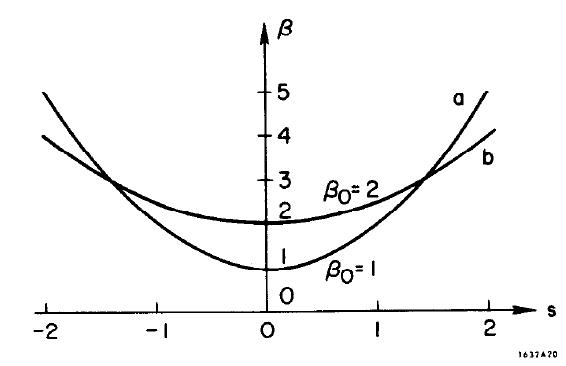
\includegraphics[width=0.8\linewidth]{./Figuras/fig20.jpeg}
	\caption{Variation of $\beta$ near the minimum that occurs in a long field free region.}
	\label{fig:fig20}
\end{figure}

Finally, observe that in a segment in which $K$ is large and $\beta'$ is not, Eq. \eqref{eq:2.80} can be approximated by
\begin{align}
	\beta'' = -2 K \beta.
\end{align}
Then, $\beta$ is a sinusoid or an exponential depending on the sign of $K$.

    \section{Disturbed closed orbits}\label{sec:2.10}

Until now I have considered the trajectories of electrons in a prescribed guide field. I wish next to consider the following question: Suppose we have analyzed the electron trajectories for this prescribed field; how will the trajectories be different if there are small deviations of the fields from the assumed prescription? In our linear approximation, the prescribed - or \emph{nominal} - guide field was specified by giving its value on the ideal orbit and its radial derivative. See Section \ref{sec:2.3}. Also, it was assumed that the field at the ideal orbit was everywhere vertical. I wish now to inquire about the effects of small deviations from the nominal field. If the vertical magnetic field at the ideal orbit differs
 from its nominal value, or if there is some small horizontal field, the lateral accelerations
will be different from what is necessary to keep an electron on the design orbit. The deviations
 of the field at the design orbit will be called \emph{field errors}. Changes in the fields which cause the focusing functions $K_x$ and $K_y$ to differ from their nominal values will, for convenience, be called \emph{gradient errors}\footnote{Although field errors will, through the term $G^2$ in Eq. \eqref{eq:2.17} also change $K_x$, such effects are not usually important.}.\\
When there are field errors, the design orbit is no longer a possible trajectory. If the errors
 are small, however, there will be another closed curve which is a possible orbit for an electron
 of the nominal energy. I shall call this trajectory the \emph{disturbed closed orbit}. The general trajectory will execute betatron oscillations with respect to this disturbed closed orbit. And the form of the betatron oscillations will be determined by the modified focussing function. That is, if we continue to let x represent the displacement from the original design orbit, we may write
\begin{align}\label{eq:2.83}
	x = x_c + x_\beta,
\end{align}
where $x_c$ is the displacement of the disturbed closed orbit from the ideal one, and $x_\beta$ is the “free” betatron oscillation about the disturbed closed orbit.\\
If the closed orbit displacements are small, our assumed linearity of the field variations means that the betatron oscillations are the same with respect to the disturbed closed orbit as they would be with respect to the design orbit. We may therefore, consider separately the distortions
 of the closed orbit caused by field errors and the disturbances to the betatron oscillations
 caused by gradient errors. And we may interpret Eq. \eqref{eq:2.83} as a superposition of the closed orbit distortion $x_c$ and a free betatron oscillation $x_\beta$ that is calculated with respect to the design orbit by the methods we have been using until now.\\
Let’s look first at the effect of the field errors. Suppose we begin by considering the effect of a field error which exists only in a small azimuthal interval $\Delta s$, which we may as well place at $s = 0$. In passing through $\Delta s$ the displacement $x$ is unchanged, but the slope $x'$ change by the amount
\begin{align*}
	\Delta x' = - \dfrac{ec\delta B}{E_0}\Delta s,
\end{align*}
where $\delta B$ is the deviation of the magnetic field from its nominal value. For the vertical
 motion we would have the same form if $\delta B$ were identified as the total radial field at the design orbit (with a suitably chosen sign). In keeping with the definition of Eq. \eqref{eq:2.3} we set $ec \delta B/E_0 = \delta G$ with a suitable subscript $x$ or $y$ implied when we are considering the radial or vertical motion. We may, as before, consider only a generic $x$-motion with the understanding that all the results apply equally to $x$-motion
 or to $y$-motion when all identifying subscripts are restored. We write, then the effect of the field error in $\Delta s$ as
\begin{align}\label{eq:2.84}
	\Delta x' = -\delta G \Delta s.
\end{align}
The field error at $s$ adds to $x'' = \Delta x'/\Delta s$ a term $\delta G$; and is, therefore, equivalent to adding a driving force $\delta G(s)$ to the equation of motion. We get the complete
equation of motion for $x_c$ by adding this new force term to the usual equation for $x$, Eq. \eqref{eq:2.31}:
\begin{align}\label{eq:2.85}
	x'' = -K(s)x -\delta G(s).
\end{align}
The displacement $x_c$ of the disturbed closed orbit is the solution of this equation
that is single valued at each physical azimuth.\\
We may make an estimate of the effect of a localized field error at $s = 0$ by using the approximate harmonic form of the betatron motion described in Section \ref{sec:2.9}. Think for the moment of an electron that is traveling along the design orbit - so that its slope $x'$ is zero. When it arrives at $s = 0$ its slope is suddenly changed to $\Delta x'$. See Fig. \ref{fig:fig21}. After $s = 0$ there is no field error (for one full revolution) so the electron begins to oscillate about the ideal orbit with the amplitude
\begin{align}\label{eq:2.86}
	b = \lambda \Delta x' = -\lambda \delta G \Delta s.
\end{align}
We may expect the closed orbit displacement $x_c$ to be of the same order of magnitude.
\begin{figure}[!htb]
	\centering
	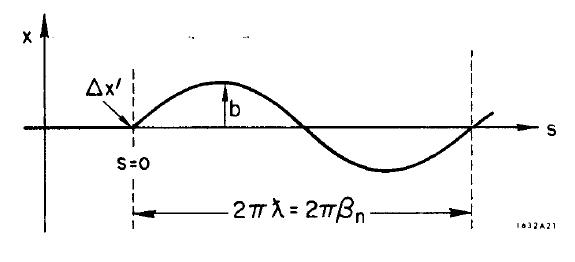
\includegraphics[width=0.8\linewidth]{./Figuras/fig21.jpeg}
	\caption{Effect of a localized field error.}
	\label{fig:fig21}
\end{figure}
To make a proper calculation of $x_c$, we should use the correct pseudo-harmonic free oscillation, and remember also that the displaced closed orbit is defined as that particular
 trajectory which closes on itself after one revolution. In other words $x_c$ must be single valued at each physical azimuth $s$, namely $x_c(s + L) = x_c(s)$. In particular,
 \begin{align}
	x_c(L) = x_c(0);
\end{align}
and by Eq. \eqref{eq:2.84},
\begin{align}
	x_c'(L) - \delta G \Delta s = x_c'(0).
\end{align}
But between $s = 0$ and $s = L$ there are no field errors, so $x_c$ is just a free oscillation about the ideal orbit. See Fig. \ref{fig:fig22}. That is, $x_c$ must be given by Eq. \eqref{eq:2.46}:
\begin{figure}[!htb]
	\centering
	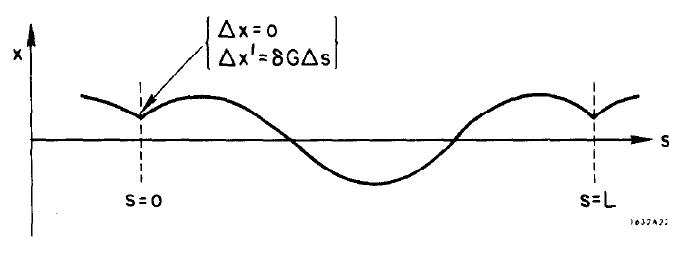
\includegraphics[width=0.8\linewidth]{./Figuras/fig22.jpeg}
	\caption{The disturbed closed orbit for a field error at $s = 0$.}
	\label{fig:fig22}
\end{figure}
Using Eq. \eqref{eq:2.52} for $x_c'(s)$ - everywhere but at $s = 0$ - you may verify that the
appropriate values of $a$ and $\vartheta$ are\footnote{The phase constant $\vartheta$ is, of course, only defined within an integral multiple of $2\pi$.}
\begin{align}
	a &= -\dfrac{\delta G \Delta s \sqrt{\beta(0)}}{2 \sin \pi \nu},\\
    \vartheta &= \pi\nu.
\end{align}

\begin{proof}
From Eq. \eqref{eq:2.52} we obtain
\begin{align*}
x_c'(s) =\dfrac{\beta'(s)x}{2\beta(s)} - \dfrac{a}{\sqrt{\beta(s)}}\sin\left(\varphi(s) - \vartheta\right).
\end{align*}
Since $x$ and $\beta$ are periodic, i.e., $x(0)=x(L)$ and $\beta(0) = \beta(L)$, $\varphi(L) - \varphi(0) = 2 \pi \nu$, by definition, and $\varphi(s=0)=0$, we use $\Delta x' =  \delta G \Delta s$,
to get the following expression
\begin{align*}
\dfrac{a}{\sqrt{\beta(0)}}\left[\sin(2\pi \nu - \vartheta) - \sin(-\vartheta)\right] = \delta G \Delta s.
\end{align*}
The terms between squared brackets can be simplified as follows
\begin{align*}
\sin(2\pi \nu - \vartheta) - \sin(-\vartheta) &= \sin(2\pi \nu)\cos\vartheta - \cos(2\pi \nu)\sin \vartheta + \sin \vartheta\\
                                         &= 2\sin(\pi \nu)\cos(\pi \nu)\cos\vartheta + \left(1-\cos(2\pi \nu)\right)\sin\vartheta\\
                                           &= 2\sin(\pi \nu)\cos(\pi \nu)\cos\vartheta + 2\sin^2(\pi \nu)\sin\vartheta\\
                                           &= 2\sin(\pi\nu)\left[\cos(\pi\nu)\cos\vartheta + \sin(\pi\nu)\cos\vartheta\right] \\
                                           &=  2\sin(\pi\nu)\cos(\pi\nu - \vartheta).
\end{align*}
Therefore
\begin{align*}
2\sin(\pi\nu)\cos(\pi\nu - \vartheta)\dfrac{a}{\sqrt{\beta(0)}} = -\delta G \Delta s,
\end{align*}
and we see that the preceding expression holds if $a = -\dfrac{\delta G \Delta s \sqrt{\beta(0)}}{2 \sin \pi \nu}$ and $\vartheta = \pi \nu$.
\end{proof}

The displacement of the disturbed closed orbit is then
\begin{align}\label{eq:2.92}
	x_c(s) = -\dfrac{\delta G \Delta s \sqrt{\beta(0)}}{2 \sin\pi\nu}\sqrt{\beta(s)}\cos\{\varphi(s)-\pi\nu\}.
\end{align}
The form of the amplitude invariant $a$ displays the two most interesting features of the disturbed closed orbit. Notice first, that the displacement of the closed orbit is everywhere
 proportional to the ``strength'' $\delta G \Delta s$ of the field error, \emph{and to the root of} $\beta(0)$, \emph{the magnitude of the betatron function at the location of the perturbation}. You see why one may consider that $\beta(s)$ or more precisely $\zeta(s) = \sqrt{\beta(s)}$ - is a measure of the ``sensitivity'' to disturbances.\\
Second, notice that the denominator of $a$ goes toward zero, and $x_c$ becomes, therefore, very large whenever the tune $\nu$ approaches an integer. It is this behavior which was referred
 to earlier as an integral resonance which must be avoided in choosing the operating point $(\nu_x, \nu_y)$.\\
Notice that the displacement of the closed orbit at the location of the error has a particularly
 simple form. You just set $s = 0$ in Eq. \eqref{eq:2.92}, or generalizing to an error $\delta G$ located in $\Delta s$ at an arbitrary azimuth, say $s_1$, you get
 \begin{align}
	x_c(s_1) = -\delta G \Delta s \dfrac{\beta{(s_1)}}{2 \tan\pi\nu}.
\end{align}
The displacement is now proportional to the first power of $\beta$, but the same resonance
dependence on $\nu$ is evident in the tangent factor. Notice also that except for the resonant denominator, this result agrees with the estimate given in Eq. \eqref{eq:2.86}.
We may also generalize Eq. \eqref{eq:2.92} to give the closed orbit distortion for an
arbitrary distribution $\delta G(s)$ of field errors around the ring. At each azimuth $s$ the closed orbit displacements caused by the errors at all other azimuths will add. For an error
 at $\bar{s} \in [0,L[$ we should replace $s = 0$ by $\bar{s}$ in Eq. \eqref{eq:2.92} - and at the same time replace $\varphi(s)$ by $\varphi(s) - \varphi(\bar{s})$, obtaining
\begin{align}\label{eq:dist_closed_orb}
x_c(s) = -\dfrac{\sqrt{\beta(\bar{s})\beta(s)}}{2\sin\pi\nu} \cos(\varphi(s)-\varphi(\bar{s})-\pi\nu)\delta G(\bar{s})\Delta\bar{s}.
\end{align}
However, we cannot sum over all $\Delta \bar{s}$ to obtain the total disturbed closed orbit, since each function has a different domain, which is $[\bar{s},\bar{s}+L[$. Note, for example, that Eq.~\eqref{eq:2.92} is valid only for $0 \leq s < L$. In order to extend the domain of the functions such that the intersection of all domains give us $[0,L[$ (the whole ring), it is sufficient to replace $\varphi(s) - \varphi(\bar{s})$, in Eq.~\eqref{eq:dist_closed_orb}, by $|\varphi(s) - \varphi(\bar{s})|$, thus extending the domain to $]\bar{s}-L,\bar{s}+L[$. One can check this by verifying that for $s \in ]\bar{s}-L,\bar{s}[$,
\begin{align*}
	\cos(|\varphi(s) - \varphi(\bar{s})| - \pi\nu) = \cos(\varphi(s+L) - \varphi(\bar{s})-\pi\nu),
\end{align*}
and for $s \in [\bar{s},\bar{s}+L[$,
\begin{align*}
\cos(|\varphi(s) - \varphi(\bar{s})| - \pi\nu) = \cos(\varphi(s) - \varphi(\bar{s}) - \pi\nu)
\end{align*}
Finally, we can add up all contributions, obtaining thus, for $s \in [0,L[$,
\begin{align}\label{eq:2.94}
	\boxed{ x_c(s) = -\dfrac{\sqrt{\beta(s)}}{2\sin\pi\nu} \oint \delta G(\bar{s}) \sqrt{\beta(\bar{s})}\cos\{ |\varphi(s) - \varphi(\bar{s})| - \pi\nu \} d\bar{s} }.
\end{align}
If we have a known field deviation $\delta G(s)$, this equation will (with $\beta(s)$ and $\nu$ taken as their undisturbed values) give us the form of the displaced closed orbit.\\
If the field deviations are true ``errors'' with an unknown statistical distribution, a more complex statistical analysis must be made to arrive at a statistical estimate of $x_c$. I shall not go into that subject here.\\
As mentioned earlier the total displacement from the ideal orbit is the sum of $x_c$ and a free betatron oscillation. In the following sections I shall ignore $x_c$ with the understanding
 that it must always be added in, when one wishes to find the total displacement of a trajectory
 from the design orbit.

 \subsection{Closed orbit correction}

 The orbit correction system in storage rings has Beam Position Monitors (BPMs) and small dipoles magnets, called correctors or steering magnets, that steer the beam depending on orbit distortions measured by the BPMs.

 The orbit distortion in the presence of localized field errors $\delta G(s_j)$ at different positions $s_j$ along the ring is given by:
	\begin{align*}
		u_c(s_i) = \dfrac{\sqrt{\beta_u(s_i)}}{2\sin\pi\nu} \sum_j \delta G({s}_j) \sqrt{\beta_u({s}_j)}\cos\{ |\varphi(s_i) - \varphi({s}_j)| - \pi\nu \},
	\end{align*}
	where $u$ may represent the $x$ or $y$ coordinate.  The orbit distortions $\Delta u(s_i)$ can be measured in localized positions $s_i$, where BPMs are installed, and localized dipolar fields $\delta G(s_j)$ (typically called ``kicks'') can be created by the correctors, also in localized positions $s_j$. The above equation can be cast in the form $\Delta u_i = \sum_{j} M_{ij}^{uu} \Delta \theta_{j}^u$ (identifying $\Delta \theta_{j}^u = \delta G(s_j)$). Therefore, one can define the orbit response matrix, whose elements can be recognized as:
 \begin{align}
 M_{ij}^{uu} = \dfrac{\sqrt{\beta_{u}(s_i)\beta_{u}(s_j)}}{2\sin\left(\pi\nu_{u}\right)}\cos\left( |\varphi_{u}(s_i) - \varphi_{u}(s_j)| - \pi\nu_{u} \right).
 \end{align}

 The orbit distortions measurements and the kick variations can be sorted in vectors as
 \begin{align*}
	 \Delta \vec{u} &= \left(\Delta x_1, \ldots, \Delta x_{\mathrm{N}_{\mathrm{BPM}}}, \Delta y_1, \ldots, \Delta y_{\mathrm{N}_{\mathrm{BPM}}}\right), \\
	 \Delta \vec{\theta} &= \left(\Delta \theta_1^x, \ldots, \Delta \theta_{\mathrm{N}_{\mathrm{CH}}}^x, \Delta \theta_1^y, \ldots, \Delta \theta_{\mathrm{N}_{\mathrm{CV}}}^y\right).
 \end{align*}

 $\mathrm{N}_{\mathrm{BPM}}$ is the number of BPMs, $\mathrm{N}_{\mathrm{CH}}$ is the number of horizontal correctors (CH) and $\mathrm{N}_{\mathrm{CV}}$ is the number of vertical correctors (CV). In this vectorial form, the orbit distortion created by the kicks variation is given by $\Delta \vec{u} = \mathbf{M} \Delta \vec{\theta}$, and the orbit response matrix has dimension $2 \mathrm{N}_{\mathrm{BPM}} \times \left(\mathrm{N}_{\mathrm{CH}} + \mathrm{N}_{\mathrm{CV}}\right)$.

 Suppose that the BPMs measure the orbit distortion $\vec{u}_{\mathrm{d}}$. With the correctors it is possible to produce an orbit variation that minimizes the 2-norm of the residual orbit. From the minimization of $||\vec{u}_{\mathrm{d}} - \mathbf{M}\Delta \vec{\theta}||^2$ with respect to $\Delta\vec{\theta}$, the required kick variations are $\Delta \vec{\theta} = -\mathbf{M}^{-1}\vec{u}_{\mathrm{d}}$. The orbit response matrix may be non-square and in these cases the symbol $\mathbf{M}^{-1}$ must be viewed as a pseudo-inverse. Since the actual problem may be non-linear, the corrections must be calculated and applied iteratively until convergence.

 The pseudo-inverse of $\mathbf{M}$ can be obtained, for example, with the method of Singular Value Decomposition (SVD), with a suitable choice of singular values used in the pseudo-inversion procedure. The SVD-based orbit correction is quite common in storage rings but there are other algorithms also available, depending on the application purpose.

    \section{Gradient errors}\label{sec:2.11}

Let’s turn now to the effects of gradient errors about the ideal closed orbit. These ``errors'' refer to the deviations of the focusing function $K(s)$ from its initially prescribed
- or nominal - value at each azimuth $s$. Let’s write
\begin{align}
	K(s)_{actual} = K(s)_{nominal} + k(s),
\end{align}
where we assume $k(s)$ to be a small quantity. The effect of the deviation $k(s)$ will be to change the betatron function from its nominal value $\beta(s)$ to some new value $\beta(s)+\Delta\beta(s)$. And the tune will be changed from its nominal value $\nu$ to some new value $\nu + \Delta\nu$. Generally the \emph{tune shift} $\Delta\nu$ is of more particular concern, because of the need to keep the operating point away from resonances.\\
Since the evaluation of $\Delta\beta$ is a bit tedious, I shall not give a rigorous deviation
here. I shall rather show how a simple calculation of $\Delta\nu$ can be made and then just write down the exact results for $\Delta\beta$ whose derivation can be found elsewhere\footnote{In any book on accelerators; see for example Ref. \cite{5} or \cite{7}.}.\\
Suppose that there is a gradient error $k$ in only a small azimuthal interval $\Delta s$ at $s = 0$. Then as an electron passes $s = 0$ it will receive an extra angular kick $\Delta x'$ which is proportional to its displacement $x$. In fact, by Eq.~\eqref{eq:2.19},
\begin{align}\label{eq:2.96}
	\Delta x' = k\, \Delta s\, x.
\end{align}
Let’s again approximate the betatron motion by a simple harmonic oscillation; and ask what will happen when an electron arrives at $s = 0$ at the maximum of an oscillation. The motion will be as shown in Fig.~\ref{fig:fig23}. Before arriving at $s = 0$ the
\begin{figure}[!htb]
	\centering
	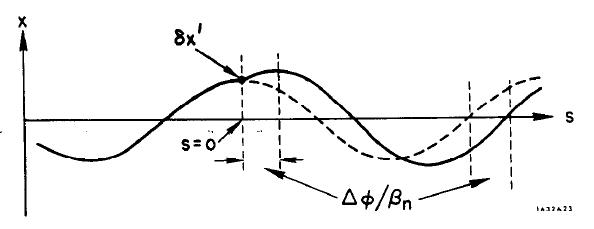
\includegraphics[width=0.8\linewidth]{./Figuras/fig23.jpeg}
	\caption{Effect of a gradient error at $s = 0$.}
	\label{fig:fig23}
\end{figure}
displacement was given by
\begin{align}
	x = b \cos s/\beta_n;
\end{align}
and after $s = 0$ it will follow
\begin{align}
	x = (b + \Delta b) \cos(s/\beta_n+\Delta\varphi),
\end{align}
where
\begin{align}
	\dfrac{b+\Delta b}{\beta_n} \sin\Delta\varphi = \Delta x'.
\end{align}
For small $\Delta x'$, $\Delta \varphi$ is small and $\Delta b$ is much less than $b$, so we can write that
\begin{align}
	\Delta \varphi \approx \dfrac{\beta_n \Delta x'}{b}.
\end{align}
Using Eq.~\eqref{eq:2.96} for $\Delta x'$ - and remembering that at $s=0$the displacement is $b$ - we have that
\begin{align}
	\Delta \varphi = \beta_n k \Delta s.
\end{align}
The effect of the gradient error is mainly to shift the phase of the oscillation by this $\Delta \varphi$. Now recall that the $2\pi\nu$ is just the total phase shift in one revolution; so roughly speaking the gradient error has produced
\begin{align}
	\Delta\nu \approx -\dfrac{\Delta\varphi}{2\pi} = - \dfrac{\beta_n k \Delta s }{2\pi}.
\end{align}
The negative sign comes in because the total phase advance has been reduced.\\
This result is actually too large by a factor of two. The reason is that we have calculated $\Delta \varphi$ for the special case of the electron arriving at $s = 0$ at the maximum
of its oscillation. If the electron arrives at $s = 0$ with the phase $\varphi_0$, the phase
shift $\Delta\varphi$ gets reduced by the factor $\cos^2\varphi_0$ - as you can easily check.
 Since on successive turns $\varphi_0$ walks through many values we should expect the average $\Delta \varphi$ to be reduced by the average of $\cos^2\varphi_0$, which is just $1/2$. With this correction we estimate a $\Delta\nu$ which is precisely what is obtained by a more direct calculation, namely
\begin{align}
	\Delta\nu = -\dfrac{1}{4\pi}\beta\, k\, \Delta s.
\end{align}
Notice that the tune shift is just proportional to the gradient error at any point and to the value of $\beta$ there. We see again that the betatron function is an indicator of the local ``sensitivity'' to imperfections of the guide field.\\
\begin{proof}
	Let $x = a\ \cos(\varphi-\vartheta)$ be the solution of the differential equation $x'' = -Kx$. For $K(s) = K(s)_{nominal}$, we've seen that an approximate solution exists, which is given by $x = b\ \cos(s/\beta_n + \varphi_0)$. When an electron passes $s=0$, its motion is now given by another differential equation: $x'' = -K(s)_{actual}\ x$ where $K(s)_{actual} = K(s)_{nominal} + k(s)$. This change on the focussing function $K(s)$ will lead to a variation $\Delta \beta$ on the betatron function. Both amplitude and phase depends on $\beta(s)$, so both of them will change too. These changes will be written as $\Delta b$ and $\Delta \varphi$, respectively. So, the solution for the new differential equation can be written as
	\begin{align*}
		x = (b+\Delta b)\ \cos(s/\beta_n + \varphi_0 + \Delta \varphi)
	\end{align*}
	You can notice that the term $\Delta \varphi$ is not multiplied by $s$, but the term $1/\beta_n$ is. The reason is that $\Delta \varphi$ only effects the electron motion in $s=0$, which is not the case for $s/\beta_n$.

	Now, considering the electron motion before the kick, we have that
	\begin{align*}
		x_i' &= -\frac{b}{\beta_n}\ \sin(s/\beta_n + \varphi_0)\\
		\therefore x_i'(0) &= -\frac{b}{\beta_n}\ \sin(\varphi_0)
	\end{align*}
	and after the kick,
	\begin{align*}
		x_f' = -\frac{b+\Delta b}{\beta_n}\ \sin(s/\beta_n + \Delta \varphi + \varphi_0)\\
		x_f'(0) = -\frac{b+\Delta b}{\beta_n}\ \sin(\Delta \varphi + \varphi_0)
	\end{align*}
	Then, the variation of $\Delta x'$ at $s=0$ is
	\begin{align*}
		\Delta x(0)' &= x(0)'_f - x(0)'_i\\
				  &= -\frac{b+\Delta b}{\beta_n}\ \sin(\Delta \varphi + \varphi_0) + \frac{b}{\beta_n}\ \sin(\varphi_0)
	\end{align*}
	Applying the angular transformation $\sin(\Delta \varphi + \varphi_0) = \sin(\Delta \varphi)\cos(\varphi_0) + \cos(\Delta \varphi)\sin(\varphi_0)$, it can be rewritten as
	\begin{align*}
		\Delta x' &= -\frac{b+\Delta b}{\beta_n}\ [\sin(\Delta \varphi)\cos(\varphi_0) + \cos(\Delta \varphi)\sin(\varphi_0)] + \frac{b}{\beta_n}\ \sin(\varphi_0)
	\end{align*}
	For small $\Delta x'$, $\Delta \varphi$ is small and we can approximate $\sin(\Delta \varphi) \approx \Delta \varphi$ and $\cos(\Delta \varphi) \approx 1$. We have that
	\begin{align*}
		\Delta x' &= -\frac{b+\Delta b}{\beta_n}\ [\Delta \varphi\ \cos(\varphi_0) + \sin(\varphi_0)] + \frac{b}{\beta_n}\ \sin(\varphi_0)\\
				  &= -\frac{b+\Delta b}{\beta_n}\ \Delta \varphi\ \cos(\varphi_0) - \frac{\Delta b}{\beta_n}\ \sin(\varphi_0)
	\end{align*}
	Discarding all second order terms,
	\begin{align*}
		\Delta x' &= -\frac{b}{\beta_n}\ \Delta \varphi\ \cos(\varphi_0) - \frac{\Delta b}{\beta_n}\ \sin(\varphi_0)
	\end{align*}
	Now, we know that the electron motion must be continuous. In other words, its motion right before the kick must be equal to its motion right after the kick, and we can write that
	\begin{align*}
		b\ \cos(\varphi_0) = (b+\Delta b)\ \cos(\Delta \varphi + \varphi_0)
	\end{align*}
	Applying the angular transformation $\cos(\Delta \varphi + \varphi_0) = \cos(\Delta \varphi)\cos(\varphi_0) - \sin(\Delta \varphi)\sin(\varphi_0)$ and approximating again $\sin(\Delta \varphi)$ and $\cos(\Delta \varphi)$, we have that
	\begin{align*}
		b\ \cos(\varphi_0) = (b+\Delta b)[\cos(\varphi_0)-\Delta \varphi\ \sin(\varphi_0)]
	\end{align*}
	It can be rewritten as
	\begin{align*}
		\frac{\Delta b}{(b+\Delta b)\Delta \varphi} = \tan(\varphi_0)
	\end{align*}
	Discarding all second order terms,
	\begin{align*}
		\frac{\Delta b}{b \Delta \varphi} &= \tan(\varphi_0)\\
		\therefore \Delta b &= b\ \Delta \varphi\ \tan(\varphi_0)
	\end{align*}
	Substituting this in the  $\Delta x'$ expression, we have that
	\begin{align*}
		\Delta x' &= -\frac{b}{\beta_n}\ \Delta \varphi\ \cos(\varphi_0) - \frac{b\ \Delta \varphi\ \tan(\varphi_0)}{\beta_n}\ \sin(\varphi_0)\\
				  &= -\frac{b}{\beta_n}\ \Delta \varphi\ \cos(\varphi_0) - \frac{b\ \Delta \varphi\ \sin^2(\varphi_0)}{\beta_n\ \cos(\varphi_0)}
	\end{align*}
	Multiplying both sides of the equation by $\cos(\varphi_0)$:
	\begin{align*}
		\cos(\varphi_0)\ \Delta x' &= -\frac{b}{\beta_n}\ \Delta \varphi\ \cos^2(\varphi_0) - \frac{b\ \Delta \varphi\ \sin^2(\varphi_0)}{\beta_n}\\
			&= -\frac{b\ \Delta \varphi}{\beta_n}[\cos^2(\varphi_0)+\sin^2(\varphi_0)]\\
			&= -\frac{b\ \Delta \varphi}{\beta_n}
	\end{align*}
	From \eqref{eq:2.96}, $\Delta x' = -k\ \Delta s\ x$. So,
	\begin{align*}
		-k\ \Delta s\ x\ \cos(\varphi_0) &= -\frac{b\ \Delta \varphi}{\beta_n}
	\end{align*}
	But we know that $x = b\ \cos(s/\beta_n + \varphi_0)$ and, of course, $x(0) = b\ \cos(\varphi_0)$. Substituting it in the mainly expression:
	\begin{align*}
		-k\ \Delta s\ b\ \cos^2(\varphi_0) &= -\frac{b\ \Delta \varphi}{\beta_n}\\
		\therefore \Delta \varphi &= \beta_n\ k\ \Delta s\ \cos^2(\varphi_0)
	\end{align*}
	From early discussions, we know that
	\begin{align*}
		\Delta \nu \approx - \frac{\Delta \varphi}{2\pi} = -\frac{\beta_n\ k\ \Delta s\ \cos^2(\varphi_0)}{2\pi}
	\end{align*}
    So, for the special case where the electron arrives at $s=0$ at the maximum of an oscillation, $\varphi_0=0$ and
    \begin{align*}
		\Delta \nu = -\frac{1}{2\pi}\beta k \Delta s
	\end{align*}
    For all other cases, we can consider the average value of $\cos^2(\varphi_0)$, which is just $1/2$. So $\Delta \varphi$ is given by
	\begin{align*}
		\Delta \nu = -\frac{1}{4\pi}\beta k \Delta s
	\end{align*}
\end{proof}
For a more rigorous deduction, check Section~\ref{sec:dtune_grad_err}.\\
If there is a gradient error $k(s)$ distributed around the ring, the total tune shift is
\begin{align}\label{eq:2.104}
	\Delta\nu = -\dfrac{1}{4\pi}\oint \beta(s) k(s) ds.
\end{align}
I have said earlier that we might expect $\Delta\nu$ to scale as $\nu$, so that large $\nu$ -
values are to be avoided. To see that it is so, recall (from Section \ref{sec:2.10}) that $\beta$ is expected to scale roughly as $|K|^{-1/2}$. Then $\nu$ should scale as $|K|^{-1/2}$. From Eq.~\eqref{eq:2.104}, $\Delta\nu$ would scale as $k\beta$ so $\Delta\nu/\nu$ would scale as $k/K$. For a given relative size of the gradient errors the tune shift $\Delta\nu$ is proportional to $\nu$. But the spacing between resonances is independent of $\nu$ so large $\nu$ values imply a more delicate machine.
A change of $\nu$ implies that there must have been a change of $\beta$ which is not evident in the simple calculation above. I shall now just write down an expression for $\Delta\beta$, and make some comments on it. It can be shown that
\begin{align}\label{eq:2.105}
	\boxed{\Delta\beta(s) = \dfrac{\beta(s)}{2\sin2\pi\nu}\oint k(\bar{s})\beta(\bar{s})\cos2\left\lbrace |\varphi(s) - \varphi(\bar{s})| - \pi\nu \right\rbrace d\bar{s}},
\end{align}
where, as usual,
\begin{align*}
	\varphi(s) = \int_0^s\dfrac{d\bar{s}}{\beta(\bar{s})}.
\end{align*}
Compare this result with the one obtained in Eq.~\eqref{eq:2.94} for the closed orbit distortions. The form is similar, but with two important differences.  First, while $\beta^{1/2}$ appears in the integral for the closed orbit displacements, the first power of $\beta$ appears in the integral for $\Delta\beta$. Second, notice that the argument of the sine factor in the denominator is now $2\pi\nu$ instead of $\pi\nu$. The resonant “blow-up” of $\Delta\beta$ occurs at both integral and half integral values of $\nu$. The gradient errors introduce
 a new set of resonances in the operating diagram of $\nu_x$ versus $\nu_y$, which must be avoided in a working storage ring.
The tune shift $\Delta\nu$ comes, of course, from the change in the betatron function. From the definition of $\nu$, Eq.~\eqref{eq:2.60}, we can write that
\begin{align}
	2\pi\Delta\nu = -\oint \dfrac{\Delta\beta(s)}{\beta^2(s)}ds.
\end{align}
A straightforward integration over $s$ of $\Delta\beta/\beta^2$ using Eq.~\eqref{eq:2.105} gives the $\Delta\nu$ of Eq.~\eqref{eq:2.104}.\\
You are perhaps by now wondering about the following strange point. Although $\Delta\beta$ has a resonance blow-up at half-integral values of $\nu$, the tune shift $\Delta\nu$ does not. How can that be? The reason is that the expression we have derived for $\Delta\nu$ applies only for small changes in $\beta$, and is therefore not valid too close to a resonance, where $\Delta\beta$ diverges. A more precise calculation, which retains second order effects in the perturbation $k$, must be made to find $\Delta\nu$ - and, in fact, $\Delta\beta$ itself - near a resonance of $\nu$.

    \section{Chromaticity}

In the last subsection, we understood how a gradient error, i.e., an error in the focusing function $K(s)$ may cause a tune shift. However, it was not discussed how such error may happen. In fact, if we look at Eq.~\eqref{eq:2.17}, one of the terms we have neglected was $K_x x \delta$, since it is a second order term. Nevertheless, we may treat this term as a first order quadrupole error $\Delta K(s) = K_x(s) \delta$. Pursuing this path, we can use Eq.~\eqref{eq:2.104} to write a contribution to the tune shift. From now on, let us assume that ${G^2 << K_1}$, so $K_x \approx K_1$ and $K_y \approx -K_1$,
\begin{align}\label{eq:Dnux_delta}
	\Delta\nu_x = \left( -\dfrac{1}{4\pi}\oint\beta_x(s) K_1(s)ds \right) \delta.
\end{align}
Using the same reasoning, we find that
\begin{align}\label{eq:Dnuy_delta}
	\Delta\nu_y = \left( \dfrac{1}{4\pi}\oint\beta_y(s) K_1(s)ds \right) \delta.
\end{align}
As a matter of fact, the quantity which is responsible to represent the variation of the tune with the energy deviation is the \emph{chromaticity} $\xi$ and it is defined as follows,
\begin{align}
	\xi = \dfrac{d\nu}{d\delta}.	
\end{align}
The part of the chromaticity which comes from the quadrupoles is called the natural chromaticity and, as expected, its formula is given by
\begin{align}
	\xi_{x,\text{nat}} &= -\dfrac{1}{4\pi}\oint\beta_x(s) K_1(s)ds,\\
   	\xi_{y,\text{nat}} &= \dfrac{1}{4\pi}\oint\beta_y(s) K_1(s)ds.
\end{align}
The natural chromaticity of a high luminosity accelerator ring is usually large. In subsection~\ref{sec:2.7} it was discussed how dangerous might be some values of tune, so it is natural to think that a wild variation of tune must be avoided. In this sense, it is important to keep $\xi$ small, despite the fact that $\xi_\text{nat}$ is large. This is one of the motivations to introduce the sextupoles in the ring, that is, to control the chromaticity.\\
For a sextupole magnetic field, where we take into account the second order magnetic field terms, we have
\begin{align}
	B_x &= B_2 x y, \label{eq:S_magx} \\ 
    B_y &= \dfrac{B_2}{2} (x^2 - y^2),\label{eq:S_magy}
\end{align}
where $B_2 = \partial^2 B_y/\partial x^2$ at $x=y=0$. We can write the magnetic field in this form by using Maxwell equations. It is easy to show that if $\nabla \times \bm{B} = 0$, then
\begin{align*}
	\dfrac{\partial^2 B_x}{\partial x \partial y} = \dfrac{\partial^2 B_y}{\partial x^2} = B_2, 
\end{align*}
and using $\nabla \cdot \bm{B} = 0$, then
\begin{align*}
	B_2 = \dfrac{\partial^2 B_x}{\partial x \partial y} = - \dfrac{\partial^2 B_y}{\partial y^2}.
\end{align*}
This allow us to write the sextupole magnetic field as in equations \eqref{eq:S_magx} and \eqref{eq:S_magy}.
As we have defined $G$, for the dipole magnetic field; $K$, for the quadrupole magnetic field, with equations \eqref{eq:2.3} and \eqref{eq:2.4}; we might, as well, define $S$, for the sextupole magnetic field as,
\begin{align}
	S(s) = -\dfrac{ec}{E_0} B_2(s).
\end{align}
Next, it is used the same steps as in subsection~\ref{sec:EqsMotion} to deduce that, by the effect of the sextupole magnetic field,
\begin{align}
	x''+ K x &= - \dfrac{S}{2} (x^2 - y^2),\\
    y''- K y &= S x y.
\end{align}
Using the fact that $x = x_{\beta} + \eta \delta$ and $y = y_{\beta}$, we may plug them into the above equations and retaining only first order terms in $x_{\beta}$ and $y_{\beta}$, it gives us
\begin{align}
	x''_{\beta} + K x_{\beta} &= - S \eta x_{\beta} \delta, \\
    y''_{\beta} - K y_{\beta} &= S \eta y_{\beta} \delta.
\end{align}
Finally, using the same reasoning to obtain equations \eqref{eq:Dnux_delta} and \eqref{eq:Dnuy_delta}, it is possible to show that
\begin{align}
	\Delta\nu_x &= \left( \dfrac{1}{4\pi}\oint\beta_x(s) S(s)\eta(s) ds \right) \delta,\\
    \Delta\nu_y &= \left( -\dfrac{1}{4\pi}\oint\beta_y(s) S(s)\eta(s) ds \right) \delta.
\end{align}
Adding up both effects in the tune, from the sextupoles and quadrupoles energy related errors, it gives us the chromaticity
\begin{align}
	\xi_x &= -\dfrac{1}{4\pi}\oint\beta_x(s)(K(s) - S(s)\eta(s)) ds, \\
    \xi_y &= \dfrac{1}{4\pi}\oint\beta_y(s)(K(s) - S(s)\eta(s)) ds.
\end{align}
Notice that, for well chosen sextupoles, i.e., $S(s)$, it is clear, looking at the equations above, that we may minimize and control the effects of the chromaticity (a.k.a. tune shift with the energy) in the ring.


\chapter{Energy Oscillations} \label{ch:3}
    \section{Off-energy Orbits}\label{sec:3.1}

In the preceding sections I have been discussing the trajectories in a storage ring of electrons with the nominal energy $E_0$ -- which is the design energy for a given setting of the magnet currents. Stored electrons do not, however, all have this ideal energy. In general, the energy $E$ of a stored electron will deviate from the nominal energy, and, as described in Section~\ref{sec:1.2}, will oscillate about it. These energy oscillations - often called “synchrotron oscillations” - are the subject of the part.\\
We must, first, understand the motion of electrons whose energy differs by a small amount $\epsilon$ from the nominal energy. Keeping the assumptions of Section~\ref{sec:EqsMotion} that the design orbit lies in a horizontal plane, energy deviations will, to first order in small quantities, affect only the radial motion. The vertical displacement will still be described by the betatron oscillations analyzed in Chapter 2, and will not be considered further here. From Section~\ref{sec:2.6} onward it was convenient to-let the symbol $x$ stand generally for either $x_\beta$ or $y_\beta$ the lateral displacements associated with the betatron oscillations. I now return to the notation in which $x$ represents the \emph{total horizontal} displacement of a trajectory from the design orbit.\\
It was shown in Section~\ref{sec:2.5} that in an ideal guide field the radial motion for
an electron with the energy deviation $\epsilon$ can be written as the sum of two parts
\begin{align}
	x = x_\beta+x_\epsilon,
\end{align}
where $x_\beta$ is the betatron displacement and $x_\epsilon$ is a displacement which depends
only on the energy of the electron. If we wish to include also the results of Section~\ref{sec:2.11}, we should include in addition, the distortion of the closed orbit due to magnet imperfections and write
\begin{align}
	x = x_\beta+x_\epsilon+x_c.
\end{align}
Since the various contributions add linearly -- under our assumptions of a linear guide field, of
 small energy deviations, and of small displacements -- we have been able to consider separately
 the several contributions to $x$. We now ignore the other contributions to $x$ and focus on $x_\epsilon$.
According to Eq.~\eqref{eq:2.28} the energy displacement $x_\epsilon$ can be written as a function of the variation of energy $\delta = \epsilon/E_0$ as follows
\begin{align} \label{eq:3.3}
	x_\epsilon = \eta(s) \delta.
\end{align}
where $\eta(s)$ is a function of the azimuthal coordinate $s$ which is single valued at
each physical azimuth. A off-energy electron with no betatron oscillations runs around a new closed orbit whose displacement from the ideal orbit is everywhere proportional to $\delta$, with a proportionality factor which depends on the azimuth according to a given function $\eta(s)$, characteristic of the total guide field configuration. I shall call $\eta(s)$ the dispersion function -- it is just the closed orbit displacement per unit energy deviation.\\
Let's look now at the nature of $\eta(s)$. It was defined -- see Eq.~\eqref{eq:2.29} -- as that
solution of the differential equation\footnote{$\eta' = d\eta/ds.$}
\begin{align}\label{eq:3.4}
	\eta'' = -K_x\eta + G(s),
\end{align}
which is $L$-periodic in $s$ and is, therefore, single valued for all physical azimuths . The functions $G(s)$ and $K_x(s)$ were defined in Eqs. \eqref{eq:2.3} and \eqref{eq:2.21}.\\
Let’s consider the qualitative behavior implied by this equation for the $\eta(s)$ of a separated function guide field (which was defined in Section~\ref{sec:2.2}. We may take
as an example the guide field of the SLAC proposal which was used for illustration in Sections \ref{sec:2.6} and \ref{sec:2.10}. In Fig. \ref{fig:fig29}(a), (b) I show $K_x$ and $G$ for this guide field and in (c), the dispersion function $\eta(s)$.
\begin{figure}[!htb]
	\centering
	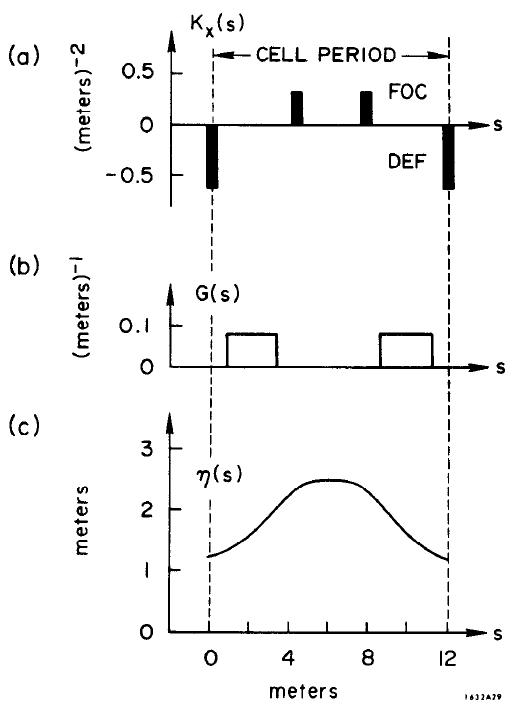
\includegraphics[width=0.8\linewidth]{./Figuras/fig29.jpeg}
	\caption{Guide-field functions and the off-momentum function for the SLAC guide field.}
	\label{fig:fig29}
\end{figure}
In a field free section both $G$ and $K_x$ are zero so $\eta(s)$ has a segment of constant
slope. In a pure quadrupole $G$ is zero and $K_x$ is just the quadrupole strength. In
a focusing quadrupole $K_x$ is positive and $\eta(s)$ follows a segment of a sinusoidal
oscillation about zero with the form
\begin{align*}
	\eta = a \cos(\sqrt{K_x}s + \vartheta).
\end{align*}
In a defocusing quadrupole $K_x$ is negative and $\eta(s)$ follows a segment of a positive
exponential like
\begin{align*}
	\eta = a \cosh(\sqrt{-K_x}s+\vartheta).
\end{align*}
The curve of $\eta(s)$ is ``attracted'' toward the $s$-axis in a focusing quad and repelled
from the axis in a defocusing quad.
Although $K_1$ is zero in a flat bending magnet, $K_x$ is not. In fact, $K_x = G^2$ and
the equation for $\eta$ is
\begin{align}
	\eta'' = -G^2\eta + G = -G^2\left( \eta - \dfrac{1}{G} \right).
\end{align}
The curve of $\eta$ is a segment of a sinusoid which is ``attracted'' toward the level
$\eta_0 = 1/G$ with a ``restoring force'' proportional to $G^2$ (The level $\eta_0$ is just equal
to the radius of curvature $\rho$ of the design orbit).\\
From the above discussion you can understand the qualitative features of the variations
 of $\eta(s)$ that appear in Fig.~\ref{fig:fig29}. For all ``normal'' storage rings it turns
out that the dispersion function is everywhere positive.\\
A storage ring user is not generally faced with the need to make a detailed calculation of $\eta(s)$. Its graph should be provided by the ring designers. I will therefore, only indicate briefly how it may be calculated. For a separated function guide field the preceding discussion can be expanded to give a method for calculating $\eta(s)$. Suppose you begin at $s = 0$ with some assumed values of $\eta(0)$ and $\eta'(0)$ and evaluate $\eta(s)$ as a succession of segments of the kind described above until you make your way around one complete revolution -- until you get to $s = L$. You will get the true $\eta(s)$ if you then choose $\eta(0)$ and $\eta'(0)$ so that $\eta(L)$ and $\eta'(L)$ are respectively, equal to $\eta(0)$ and $\eta'(0)$. The computation can be carried out most straightforwardly by using a matrix technique (See Ref. \cite{11}).\\
The dispersion function can also be obtained (for any kind of guide field) by making use of the results we obtained in Section~\ref{sec:2.11} for disturbed closed orbits. We may imagine that an off-energy orbit is just a ``disturbed'' closed orbit since an energy deviation gives rise to a change in curvature just as does a field error. That is to say, that a field error $\Delta G$ in a segment $\Delta s$ of the orbit produces a change of curvature in the path of an electron of energy $E_0$ which is the same as the change of curvature that results when an electron with an energy deviation $\delta$ goes through the nominal field provided that $\Delta G/G = \delta$. Since $\eta(s)$ is the ratio of the closed orbit displacement to $\delta$, we may compute $\eta(s)$ by replacing $\Delta G$ in Eq.~\eqref{eq:2.92} of Section~\ref{sec:2.11} by $G$. This argument can also be justified by noticing that Eq.~\eqref{eq:3.4} for $\eta$ has the same form as Eq.~\eqref{eq:2.85} for $x_c$ in Section~\ref{sec:2.11}; the latter going into the former if we make the substitutions $x_c \to \eta\delta$ and $-\Delta G \to G\delta$. Making the same substitutions in Eq.~\eqref{eq:2.94} we get
\begin{align}
	\boxed{ \eta(s) = \dfrac{\sqrt{\beta(s)}}{2\sin{(\pi\nu)}}\oint G(\bar{s})\sqrt{\beta(\bar{s})}\cos\left\lbrace |\varphi(s) - \varphi(\bar{s})| - \pi\nu \right\rbrace d\bar{s}}.
\end{align}
So if $\beta(s)$ is already known we can get $\eta(s)$ by an integration. Notice that $\eta(s)$ too will have a resonance behavior when $\nu$ approaches an integer.\\
If the design orbit does not lie in a plane - as, for example, in the recent DESY or Orsay designs - then the discussion of this Section must be repeated for the vertical displacements. There will in such cases be two curvature functions $G_x$ and $G_y$ as well as the two focussing functions $K_x$ and $K_y$. The vertical displacements will also have an off-energy contribution which will be proportional to an dispersion function $\eta_y(s)$. And this vertical dispersion function can be evaluated in terms of the vertical focusing and curvature functions. There will be generally one important qualitative difference from the horizontal case in that $\eta_y$, will have both positive and negative values and its average around the ring will be zero.

    \section{Orbit length: momentum compaction}\label{sec:3.2}

An important consequence of an energy deviation is the associated change in the circumference
 of the closed orbit. I wish now to take a look at this effect. An electron of the nominal energy $E_0$. which circulates on the design orbit will, in one revolution, travel the distance $L$, the circumference of the design orbit. On any other trajectory, the path length traveled in one revolution will depend on the deviations from the ideal orbit and may be expected to differ from $L$. We have already noticed in Section~\ref{sec:2.4} that an electron which moves from $s$ to $s + ds$ with a displacement $x$ from the design orbit has a path length $d\ell$ different from $ds$ by an amount that depends on the local radius of curvature. See Fig.~\ref{fig:fig9}. We found there - Eq.~\eqref{eq:2.15} - that
\begin{align} \label{eq:3.7}
	d\ell = (1 + G(s)x) ds,
\end{align}
so long as only terms to first order in $x$ are retained.\\
A betatron oscillation will produce on the average no first order change in the path length. The path is lengthened on a positive swing ($x > 0$) of the oscillation and shortened on a negative swing. Since the betatron displacements are on the average, symmetric about $x = 0$, the path length change is zero when averaged over one or more complete betatron cycles. If the tune $\nu$ is much greater than $1$ so that there are several betatron cycles in one revolution, the net
change in the path length in one revolution is small. If $\nu = 1$ however, there will be changes in the path length from one revolution to the next. We shall however, be interested here only on the average path length (averaged over several revolutions) and the betatron oscillations will not, to first order, affect this average.\\
There is a second order effect - which gives a time change proportional to the square of the betatron amplitude. It can introduce a very small coupling between betatron oscillations
 and energy oscillations. I am ignoring here all such second-order processes.\\
 The lateral displacement $x_\epsilon$ of an off-energy orbit does give rise to a change in
the orbit length - because, for a given energy deviation, $x_\epsilon$ has generally the same
sign all around the ring. Putting $x_\epsilon$ for $x$ in Eq.~\eqref{eq:3.7} and integrating
once around the ring, we get for the circumference $\ell_\epsilon$ of an off-energy
closed orbit
\begin{align}
	\ell_\epsilon = \oint d\ell = \oint (1 + G(s)x_\epsilon)ds.
\end{align}
The first term of the integral gives the complete integral of $ds$ which is just $L$, the length of the design orbit. The second term gives the elongation due to the energy deviation; let's call it $\delta \ell_\epsilon$. Recalling Eq.~\eqref{eq:3.3} for $x_\epsilon$, we get that
\begin{align} \label{eq:3.9}
	\delta\ell_\epsilon = \dfrac{\epsilon}{E_0} \oint G(s) \eta(s) ds.
\end{align}
The change in the orbit length is proportional to the energy deviation $\epsilon$, with a constant of proportionality - the definite integral - which can be obtained from the known properties of the guide field.\\
It is convenient to define a dimensionless parameter $\alpha$, which we may call the momentum compaction by
\begin{align}\label{eq:3.10}
	\dfrac{\delta \ell_\epsilon}{L} = \alpha \dfrac{\epsilon}{E_0}.
\end{align}
It follows from Eq.~\eqref{eq:3.9} that
\begin{align}\label{eq:3.11}
	\alpha = \dfrac{1}{L} \oint G(s) \eta(s) ds.
\end{align}
The momentum compaction $\alpha$ is a number which like the betatron number $\nu$ is a characteristic of the total guide field. It is a crucial parameter of the energy oscillations.\\
In the literature, the momentum compaction is usually defined by the relation between the normalized variation of $\ell$ and the normalized variation of the momentum. However, it is acceptable to define as in Eq.~\eqref{eq:3.10}, because when the speed of the particle $v$ approaches the speed of light $c$, these quantities converge to each other, as it is shown below.\\
From relativistic mechanics, we know that
\begin{align}\label{eq:}
	E^2 = p^2c^2 + m_0^2 c^4,
\end{align}
Then, for a small energy deviation we have
\begin{align}
	2 E \delta E = 2p \,\delta p \, c^2,
\end{align}
which can be written as
\begin{align}
	\dfrac{\delta E}{E} = \dfrac{p^2 c^2}{E^2} \dfrac{\delta p}{p}.
\end{align}
this equation can be simplified by using the relation $p = \gamma m_0 v$ and $E = \gamma m_0 c^2$, where $\gamma = (1 - v^2/c^2)^{-1/2}$, as follows
\begin{align}\label{eq:E=P}
	\dfrac{\delta E}{E} = \left( \dfrac{v}{c} \right)^2 \dfrac{\delta p}{p}.
\end{align}
Then, if $v \to c$, $\frac{\delta E}{E} = \frac{\delta p}{p}$.
We can get a little better understanding of the nature of $\alpha$ by looking at it for the most common kind of guide field, the isomagnetic guide field defined earlier. In an isomagnetic field, $G$ has the value $G_0$ in all magnets and zero elsewhere (see Eq.~\eqref{eq:2.9}) so Eq.~\eqref{eq:3.11} can be expressed by
\begin{align} \label{eq:3.12}
	\alpha = \dfrac{G_0}{L} \int_{\text{Mag}} \eta(s) ds. \hspace{5mm} \text{(isomag.)}
\end{align}
where the integral is to be taken over only those parts of the design orbit which
are in the bending magnets.\\
This result can be written in a more illuminating way. Suppose we define the magnetic average of $\eta$ as
\begin{align} \label{eq:3.13}
	\left\langle \eta \right\rangle_{\text{Mag}} = \dfrac{1}{\ell_{\text{Mag}}} \int_{\text{Mag}} \eta(s) ds.
\end{align}
where $\ell_{\text{Mag}}$ is the total length of the orbit segments in the bending magnets (This would be the usual definition of the mean value of $\eta$ in all the magnets).
But all of the bending magnets must add up to a complete circle so $\ell_{\text{Mag}}$ is just $2\pi$ times the constant orbit radius $\rho_0$ in the magnets which is just $1/G_0$; so
\begin{align} \label{eq:3.14}
	\alpha = \dfrac{2\pi}{L} \left\langle \eta \right\rangle_{\text{Mag}}.
\end{align}
Let the time required to complete one turn in the design orbit be $T$. Then, the time required for a given electron, which has a small energy deviation, to give one complete turn is given by
\begin{align}
	T + \delta T = \dfrac{L + \delta \ell_\epsilon}{v + \delta v}.
\end{align}
which can be written with a first order approximation as
\begin{align}\label{eq:T_E}
	\dfrac{\delta T}{T} &= \dfrac{\delta \ell_\epsilon}{L} - \dfrac{\delta v}{v}\\
    					&= \alpha \dfrac{\delta E}{E} - \dfrac{\delta v}{v}.
\end{align}
Using relativistic mechanics again, it is possible to relate $\delta v$ with $\delta p$. Taking a small momentum deviation in the equation $p = \gamma m_0 v$, one obtains that
\begin{align*}
	\delta p &= \left(\gamma m_0 + m_0 v \frac{d\gamma}{dv}\right)\delta v\\
    		&= \left(\gamma m_0 v + m_0 \frac{v^2}{c^2} \gamma^3 v \right) \dfrac{\delta v}{v}.
\end{align*}
Using the relation $p = \gamma m_0 v$ once again,
\begin{align*}
	\dfrac{\delta p}{p} &= \left( 1 + \dfrac{v^2}{c^2}\gamma^2 \right) \dfrac{\delta v}{v}\\
    					&= \gamma^2 \dfrac{\delta v}{v}.
\end{align*}
Using Eq.~\eqref{eq:E=P}, it follows that
\begin{align}
	\dfrac{\delta E}{E} = \left( \dfrac{v}{c}\gamma \right)^2 \dfrac{\delta v}{v}.
\end{align}
Finally, we plug this in Eq.~\eqref{eq:T_E} and obtain
\begin{align}
	\dfrac{\delta T}{T} = \left( \alpha - \dfrac{1}{(v/c)^2\gamma^2} \right)\dfrac{\delta E}{E}.
\end{align}
As $v$ approaches $c$, which is the case for accelerator rings, the above relation simplifies to
\begin{align} \label{eq:3.15}
\frac{\delta T}{T} = \alpha \frac{\delta E}{E}.
\end{align}
It is interesting to notice that there exists a $v$ such that the multiplicative term of the energy deviation vanishes. In this case we have an isochronous behavior, since the time that the particle takes to complete one revolution does not change with an energy deviation.

    \section{Energy loss and gain}\label{sec:3.4}
Until now we have ignored those effects which change the energy of a stored electron; it is now necessary to consider the processes by which an electron loses or gains energy. The lateral acceleration along the curved parts of a trajectory causes an electron to radiate away some of its energy. The characteristics of this radiation loss will be discussed in some detail in Sect. \ref{sec:4.1}. If the electron is to remain captured in the storage ring this radiation loss must be compensated for, on the average, by an equal energy gain from the radio frequency accelerating system of the ring -- one or more electrode structures which produce, along parts of the orbit, an electric field that can feed energy to the moving electron. It is the interplay of the radiation loss and the acceleration gain -- together with the properties of the guide field -- that gathers injected electrons into stable circulating bunches and is responsible for the residual small energy oscillations of the electrons in a bunch.

An electron of the nominal energy $E_0$, moving on the design orbit will radiate away a certain amount of energy, say $U_0$, each revolution. This radiation loss is always a very small fraction (typically $10^{-4}$ or less) of the electron's energy. And the energy gain from the acceleration system is of course, of the same order. The small magnitude of the loss in one revolution allows us, fortunately, to make a number of simplifying assumptions without which a study of the energy oscillations would hardly be tractable. We may, to begin with, make the approximation that an electron which starts a revolution with the energy $E_0$ will also loose the energy $U_0$ during the revolution. Although the energy will not strictly remain at $E_0$, nor the trajectory remain on the design orbit, the deviations during one revolution can be neglected. The effects which accumulate over several revolutions must, however, be taken into account.

If an electron with the energy $E_0$ is given a betatron oscillation its instantaneous rate of radiation loss may change -- because of a different lateral acceleration along the trajectory. But the average energy loss over a complete betatron oscillation will not change to first order in the betatron amplitude. (Changes in the lateral oscillation will be proportional to $x$ and will, to first order, average to zero over a complete
cycle). Since we shall be satisfied to consider only the effects which occur over many betatron oscillations, we need to look only at the average energy loss. So long as we are keeping to our first order view of a storage ring we may ignore any dependence of the radiation loss on the betatron displacements.

The radiation loss will however, change with a change in the energy of an electron. Both its different trajectory and its different energy can contribute to a modified energy loss. Because all energy changes occur slowly, we may consider that an electron is at any instant moving on the dispersion closed orbit which corresponds to its instantaneous energy -- or is performing free betatron oscillations about that orbit. Since we know the form of the dispersion orbit, we can compute the energy lost in each revolution. I shall consider this problem later (in \autoref{sec:4.1}); for now we may take it as a given function $U_{rad}(\epsilon)$ of the energy deviation $\epsilon$.

Since we shall generally be interested only in small energy deviations, we need keep only the linear term in the variation of $U_{rad}$ and write that
\begin{align}
	U_{rad} = U_0 + D\epsilon\label{eq:3.23}
\end{align}
where
\begin{align} \label{eq:3.24}
	D = \left(\frac{dU_{rad}}{d\epsilon}\right)_0
\end{align}
and the derivative is evaluated at the nominal energy $E_0$. For the present, then, the radiation loss may be described by the two constants $U_0$ and $D$ -- which will be evaluated in terms of the properties of the guide field in Chapter \ref{ch:4}.

Let's now turn to the radio frequency accelerating system -- “rf system” for short -- which supplies energy to the electrons to compensate for the radiation loss. The rf system consists typically of one or more cavity resonators such as the one shown schematically in \autoref{fig:fig30}, disposed at various places around the storage ring
and supplied with rf power from some synchronized radio power sources. These cavities produce oscillating electric fields along the electron trajectories; and it is the component of these fields along the electron's path which feeds energy to the electrons. An electron which goes around once on the design orbit will be given by the rf system an amount of energy $U_{rf}$ equal to the integral of the instantaneous electric force along its trajectory.

 \begin{figure}[!htb]
 	\centering
 	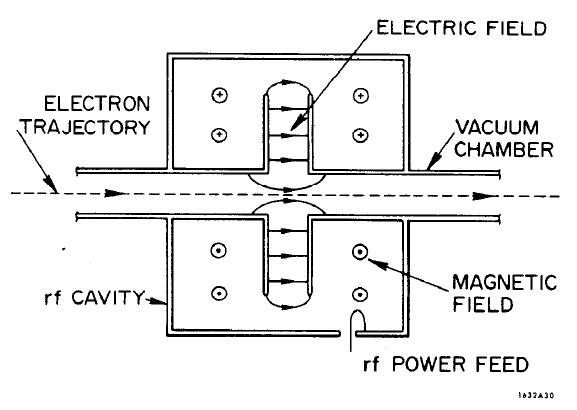
\includegraphics[width=0.7\linewidth]{./Figuras/fig30.jpeg}
 	\caption{Schematic diagram of an rf accelerating cavity.}
 	\label{fig:fig30}
 \end{figure}

Since the rf fields are time varying, \footnote{As they must be if there is to be a net integral of the electric field around a closed path!}the energy gained by an electron in making one circuit around the ring will depend on the time at which that circuit begins in relation to the oscillations of the accelerating fields. Let's say that the time dependence of the fields is given. Then the energy $U_{rf}$ gained by the electron -- in one revolution will depend on the time1 that it starts its revolution. (We may take that the revolution starts at some reference azimuth, say $s = 0$.)

If electrons are to be stored on (or near) the design orbit, the variation of $U_{rf}(\bar{t})$ must have certain characteristics. I shall assume that $U_{rf}(\bar{t}$) is a periodic function with a period that is some integral submultiple of the period $T_0$, the period of revolution of an electron that circulates on the design orbit. That is,
\begin{align}
	U_{rf}(\bar{t}+T_0/k) = U_{rf}(\bar{t})\label{eq:3.25}
\end{align}
where $k$ is some integer that will be called the harmonic number of the rf system. The variation of $U_{rf}(\bar{t})$ might be, for example, like the function shown in \autoref{fig:fig31}. (Although the assumed time variation of $U_{rf}$ is somewhat more restrictive than necessary, the rf fields must have at least similar characteristics if a storage ring is to work. And most storage rings will have generally the characteristics assumed.)

\begin{figure}[!htb]
	\centering
	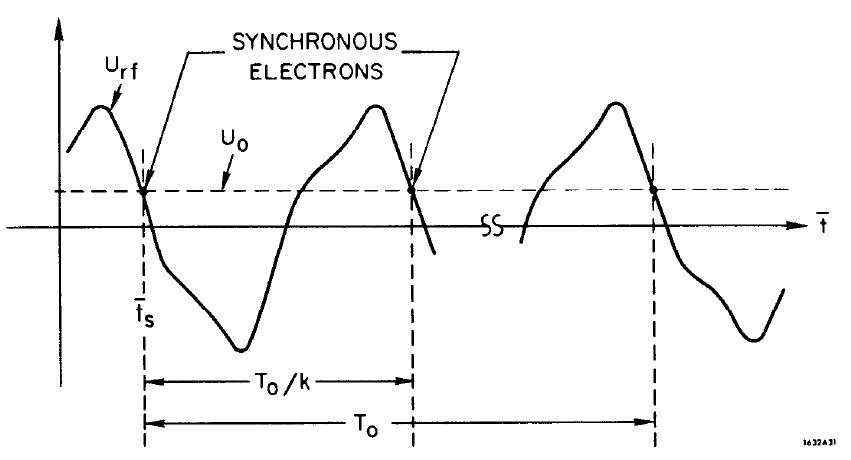
\includegraphics[width=0.85\linewidth]{./Figuras/fig31.jpeg}
	\caption{Energy gain from the rf system as a function of the starting time t of a revolution.}
	\label{fig:fig31}
\end{figure}

Now consider what can happen with an electron of the nominal energy $E_0$ that is circulating on the design orbit. Suppose that it is started on its journey at just the right time $\bar{t}_s$ for which the rf gain $U_{rf}(\bar{t}_s)$ is just equal to the radiation loss $U_0$. See \autoref{fig:fig31}. In the next revolution the energy lost and gained will compensate and the electron will return to its starting point again with the energy $E_0$. The time taken for the revolution is $T_0$; so the electron will start the next revolution at the time $\bar{t}_s + T_0$ and by Eq. \eqref{eq:3.25} the rf gain will again be equal to $U_0$. The electron will continue to circulate indefinitely on the design orbit. Such an electron which passes the reference azimuth at the times $\bar{t}_s + jT_0$ (where $j$ = 1,2,3,..) is called a synchronous electron -- because its rotation is synchronous with the oscillating rf fields. And $\bar{t}_s$ is generally called the synchronous phase of the rf system. (Of course with a periodic rf there are equivalent synchronous starting times once each rf period.)

I have clearly assumed that the peak value of $U_{rf}$ is greater than the radiation loss $U_0$ of the synchronous electron. It follows that there will, in actuality, be
two possible choices (at least) of $\bar{t}_s$ in each cycle of $U_{rf}$ -- one where $U_{rf}$ has a positive slope and one where it has a negative slope. Only one of the two -- the one where the slope is negative -- corresponds to a phase of stable equilibrium, as you will presently see. So only that one will be designated as the synchronous phase $\bar{t}_s$. You can also see from \autoref{fig:fig31} that with a rf harmonic number $k$ there will be $k$ different synchronous starting times -- and therefore, $k$ distinguishable synchronous electrons. These $k$ synchronous phases correspond to $k$ possible stored bunches of electrons.

An electron which is moving with a lateral displacement from the design orbit will see somewhat different electric fields than one moving on the design orbit. It is generally true, however, that its energy gain in one complete revolution -- the path integral of the electric force -- depends very little on the lateral displacements. I shall therefore ignore any dependence of the energy gain on such lateral displacements -- whether they are due to energy deviations or to betatron oscillations -- and consider only the important variation of the energy gain with the starting time $\bar{t}$.

The circulating position of a synchronous electron provides a convenient reference point for the study of the longitudinal oscillations of the electrons in a bunch. We may indeed refer to the moving position of the synchronous electron as the “center” of the bunch and describe the instantaneous azimuthal position of any other electron of the bunch by giving its longitudinal displacement $y$ from the bunch center. That is, we define
\begin{align}
	y(t) = s(t) - s_c(t)
\end{align}
where $s$ is the azimuthal position of any particular electron and $s_c$ refers to the position of the bunch center. See \autoref{fig:fig32}.

\begin{figure}[!htb]
	\centering
	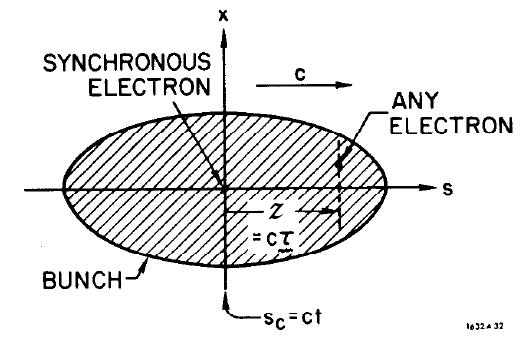
\includegraphics[width=0.6\linewidth]{./Figuras/fig32.jpeg}
	\caption{The longitudinal coordinates $y$ and $\tau$ of an electron in a bunch.}
	\label{fig:fig32}
\end{figure}

For the present discussion I find it somewhat more convenient to describe the longitudinal motion by an equivalent variable $\tau$ defined simply by
\begin{align}
	\tau(t) = y(t)/c
\end{align}
which I shall call the time displacement from the center of the bunch. (The time displacement is very nearly equal to the time interval $\Delta t$ between the arrival of an electron at any particular azimuth and the arrival of the synchronous electron. The difference is equal to the change of $\tau$ in the time $\Delta t = - \tau$ which because of the slow rate of change of $\tau$ can be ignored.) Notice that the time displacement $\tau$ is positive when an electron arrives at each azimuth ahead of the synchronous electron and $\Delta t$ is negative, since it arrives before the synchronous electron.

Because of the time variations of the rf accelerating fields only a synchronous electron will receive the energy $U_0$ each revolution. Any other electron will gain in one revolution an energy $U_{rf}$ which depends on its time displacement $\tau$. We may follow the conventional notation and write
\begin{align}
	U_{rf} = eV(\tau)
\end{align}
where $e$ is the electronic charge and $V(\tau)$ is called the ``rf voltagel'' -- by analogy with a dc accelerating system. The form of $V(\tau)$ is of course related to $U_{rf}(\tau)$; specifically,
\begin{align}
	eV(\tau) = U_{rf}(\bar{t}_s + \Delta t) = U_{rf}(\bar{t}_s - \tau)
\end{align}
The variation with $\tau$ is reversed from the variation with $\bar{t}$ so the energy gain function of \autoref{fig:fig31} would give the $V(\tau)$ shown in \autoref{fig:fig33} -- where now $\tau = 0$ corresponds to the time displacement of a synchronous electron. Notice that the slope of $V(\tau)$ is positive at $\tau = 0$.

\begin{figure}[!htb]
	\centering
	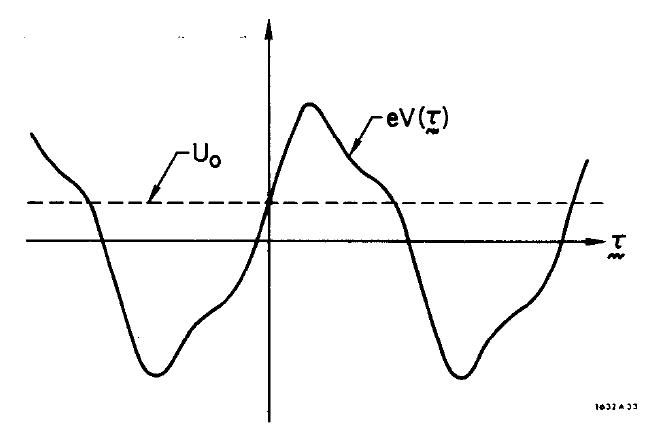
\includegraphics[width=0.6\linewidth]{./Figuras/fig33.jpeg}
	\caption{The rf voltage function $V(\tau)$.}
	\label{fig:fig33}
\end{figure}

It should perhaps be emphasized that the effective ``voltage'' of a multiple cavity system typical of high energy rings is not simply related to any observable electric ``voltage'' but depends on the relative positions and oscillation phases of the various rf cavities in the system. The voltage $V(\tau)$ may in fact, depend on the sense of circulation around the ring and may therefore, be quite different for electrons circulating one way around the ring and positrons circulating in the opposite direction.

We are now ready to consider the energy oscillations of an electron in a circulating bunch in a storage ring. Let's first see qualitatively what will happen. Suppose an electron has initially the nominal energy $E_0$ but a positive time displacement $\tau$ -- so that it is ahead of the synchronous position. The radiation loss depends only on the energy so it will be $U_0$ each revolution. But the energy gain will be greater than $U_0$. The electron will gain a little bit of energy each revolution. But an increase in energy will, by Eq. \eqref{eq:3.15}, cause its revolution time to get longer; and its time advance with respect to the bunch center will, accordingly, begin to decrease. After some revolutions the time displacement will decrease to zero. But, by then, the electron's energy will be higher than the nominal energy $E_0$ since the electron has continually been gaining energy -- so the time displacement will continue to decrease now toward negative values of $\tau$. At negative values of $\tau$ however, the energy gain will be too small to compensate for the energy loss by radiation and the electron's energy will begin to decrease toward the nominal energy. When the nominal energy is reached, the time displacement will stop decreasing; but, since it is then negative the energy gain per revolution is below $U_0$ and the energy will begin dropping below $E_0$. Now the time displacement will begin returning toward zero. The process will continue until $\tau$ returns to its starting value, at which point the energy will again be $E_0$.

Let's put this description into quantitative terms. First, take the variation of the time displacement $\tau$. It is convenient to keep track of what is happening by observing a bunch once each revolution when the bunch center is at some arbitrarily chosen reference point. The discussion will be easiest if we take the reference point in some field free region (away from any magnets or rf cavities). In \autoref{fig:fig34} I show two “pictures” of the same bunch on two successive passages of the reference azimuth. In each picture the bunch center is at the reference azimuth so the time between the two pictures is just $T_0$ the revolution time on the design orbit.

\begin{figure}[!htb]
	\centering
	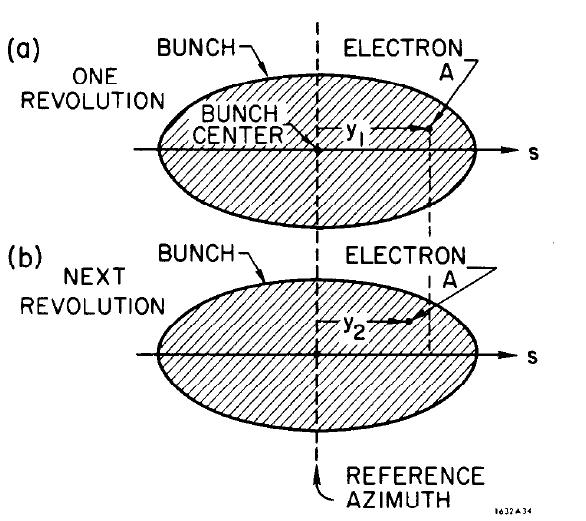
\includegraphics[width=0.6\linewidth]{./Figuras/fig34.jpeg}
	\caption{Longitudinal motion of an electron within a bunch.}
	\label{fig:fig34}
\end{figure}

The pictures show also the position of some particular electron of the bunch: “Electron A”. In the first picture Electron A is ahead of the bunch center by the distance $y_1$. In the second picture the longitudinal displacement has decreased to $y_2$. Between the two pictures the bunch center has traveled once around the design orbit, a distance $L=cT_0$. And since Electron A travels also at the speed $c$, it also has covered a path length equal to $L$. But if it has an energy deviation $\epsilon$ from the nominal energy, the path length for one complete revolution (back to $y_1$) -- would be, as shown in \autoref{sec:3.2}, greater than $L$ by the amount $\delta \ell$ with
\begin{align}
	\frac{\delta \ell}{L} = \alpha\frac{\epsilon}{E_0}
\end{align}
Electron A fails to reach its previous azimuth by the small distance $\delta y = -\delta \ell$, so
\begin{align}
	y_2 - y_1 = \delta y = -\alpha \frac{\epsilon}{E_0}L
\end{align}
The change $\tau$ during the revolution $n$ is
\begin{align}
	\Delta \tau_{n+1} = \frac{\delta y}{c} = -\alpha \frac{\epsilon_n}{E_0}\frac{L}{c} = -\alpha\frac{\epsilon_n}{E_0}T_0
\end{align}
Since the time between the two pictures is $T_0$ the time rate-of-change of $\tau$ is $\Delta \tau/T_0$ or
\begin{align}
	\frac{d \tau}{dt} = -\alpha \frac{\epsilon}{E_0}\label{eq:3.32}
\end{align}
A nice, simple result.

Next, the energy variation. During its revolution Electron A has lost by radiation the energy $U_{rad}(\epsilon)$ and gained from the rf system the energy $eV(\tau)$. The net change in energy during the revolution $n$ is then,
\begin{align}
	\Delta \epsilon_{n+1} = eV(\tau_n)-U_{rad}(\epsilon_n)
\end{align}
The rate-of-change of the energy deviation $\epsilon$ -- when averaged over a complete revolution -- is $\Delta \epsilon/T_0$ so we have that
\begin{align}
	\frac{d\epsilon}{dt} = \frac{eV(\tau)-U_{rad}(\epsilon)}{T_0}\label{eq:3.34}
\end{align}
(We may drop the subscripts on $\tau$ and $\epsilon$ because we may now take it as continuous and derivable variables, since their variation each turn with $T_0$ is sufficiently small, we obtain them by a smooth interpolation from $\tau_1$ to $\tau_2$ to $\tau_3$, etc and $\epsilon_1$ to $\epsilon_2$ to $\epsilon_3$, etc).

The two coupled equations, \eqref{eq:3.32} and \eqref{eq:3.34} describe the energy oscillations -- and the associated oscillations of the time displacement -- of a stored electron. They must be solved together to give the time variation of $\epsilon$ and of $\tau$.

It will turn out -- unfortunately -- that the time displacements which are associated with small energy deviations need not themselves be ``small'', in the sense that they may span a significant fraction of a complete cycle of the variation of $V(\tau)$. This will be the one instance in which we may not look only at linear terms. We shall need at times to take into account the full nonlinear variations of $V(\tau)$. At other times, however, we shall wish to focus our attention on the small energy oscillations which correspond also to small time displacements. For such oscillations we shall need to retain only the linear part of the variation of $V(\tau)$. Since the acceleration energy gain at $\tau = 0$ is by definition $U_0$, we may then write
\begin{align}
	U_{rf} = eV(\tau) = U_0 + e\dot{V}_0\tau\label{eq:3.35}
\end{align}
where $\dot{V}_0$ stands for $dV/d\tau$ evaluated at $\tau=0$.

It is quite common for the rf voltage of a storage ring to have a sinusoidal variation with time. In such cases we would have that
\begin{align}\label{eq:3.36}
	V(\tau) = \widehat{V} \sin(\omega_{rf}(\tau+\tau_0))
\end{align}
where $\widehat{V}$ is called the ``peak rf voltage'' and $\omega_{rf}\tau_0$  is called the ``synchronous rf phase angle''. With our assumptions
\begin{align}
	\omega_{rf} = 2\pi \frac{k}{T_0} = k\omega_r
\end{align}
It also follows that
\begin{align}
	\omega_{rf}\tau_0 = \arcsin(U_0/e\widehat{V})
\end{align}
and that
\begin{align}
	\dot{V}_0 = \omega_{rf}\widehat{V}cos(\omega_{rf}\tau_0) = \omega_{rf}\widehat{V}\left[1-\left(\frac{U_0}{e\widehat{V}}\right)^2\right]^{1/2}
\end{align}

    \section{Small oscillations}\label{sec:3.5}
%\subsection{Aproximação para a órbita fechada e a compactação de momento}
We are now ready to analyse in detail the energy oscillations of the electrons in a bunch. I shall take up first the special case of the small (linearized) oscillations which occur so long as the variations of $\tau$ are limited to a small interval that corresponds to an approximately linear segment of $V(\tau)$. And then look later (in the following section) at the nonlinear oscillations which occur when the excursions of $\tau$ are large.

For small $\tau$ and $\epsilon$, we may replace $V(\tau)$ and $U_{rad}(\epsilon)$ by the linear approximations of Eqs. \eqref{eq:3.35} and \eqref{eq:3.23}. Then Eq. \eqref{eq:3.34} becomes
\begin{align}
	\frac{d\epsilon}{dt} = \frac{1}{T_0}(e\dot{V}_0 \tau - D\epsilon)\label{eq:3.40}
\end{align}
This equation can now be combined with Eq. \eqref{eq:3.32} to give a differential equation for $\epsilon$ or $\tau$. Suppose we choose $\tau$. Taking the time derivative of Eq. \eqref{eq:3.32} and eliminating $\epsilon$, you can show that
\begin{align}
	\frac{d^2 \tau}{dt^2} + 2\alpha_\epsilon \frac{d\tau}{dt} + \Omega^2 \tau = 0\label{eq:3.41}
\end{align}
with \footnote{Careful! There are not enough different letters. The constant $\alpha_\epsilon$ is a new quantity quite distinct from the dilation factor $\alpha$.}
\begin{align}
	\alpha_\epsilon &= \frac{D}{2 T_0}\\
	\Omega^2 &= \frac{\alpha\ e\ \dot{V}_0}{T_0\ E_0} \label{eq:3.43}
\end{align}

You will recognize that Eq. \eqref{eq:3.41} describes a damped harmonic oscillation with the oscillation (angular) frequency $\Omega$, and damping coefficient $\alpha_\epsilon$. Since the damping rate in a storage ring is always slow ($\alpha_\epsilon << \Omega$) the solution of Eq. \eqref{eq:3.41} can be written as
\begin{align} \label{eq:3.44}
	\tau(t) = A\ e^{-\alpha_\epsilon t} \cos(\Omega t - \theta_0)
\end{align}
with $A$ e $\theta_0$ arbitrary constants. Or, using the usual complex notation,
\begin{align}
	\tau(t) = \tilde{\tau}\ e^{-(\alpha_\epsilon - i\Omega)t}
\end{align}
where $\tilde{\tau}$ is a complex constant.

Equations \eqref{eq:3.40} and \eqref{eq:3.32} can be solved instead for $\epsilon$, which, you can show, satisfies the same differential equation as $\tau$, Eq. \eqref{eq:3.41}. And so the time variations of $\epsilon$ are
\begin{align}
	\epsilon(t) = \tilde{\epsilon}\ e^{-(\alpha_\epsilon - i\Omega)t}
\end{align}
From Eq. \eqref{eq:3.32} $\tilde{\epsilon}$ and $\tilde{\tau}$ are related by
\begin{align}
	\tilde{\epsilon} = -i\frac{\Omega E_0}{\alpha}\tilde{\tau}\label{eq:3.47}
\end{align}
(because $\alpha_\epsilon << \Omega$) and so the oscillations of $\epsilon$ and $\tau$ will have a phase difference of $\pi/2$.

Notice that the oscillation frequency of the small energy oscillations depends on the rf system only through $\dot{V}_0$. The frequency is proportional to the square root of the rf slope at the synchronous phase. The other parameters, $\alpha$, $T_0$, $E_0$ are characteristics of the guide field (including the energy at which it is operated). The damping constant of the energy oscillations $\alpha_\epsilon$ -- which is the inverse of the damping time constant - is proportional to $D$, which is the rate-of-change of the radiation loss with energy. As we shall see, this rate depends on the electron energy and on the properties of the guide field.

I would like to give now some orders of magnitude for the various quantities which have been appearing. The skeptical among you may then be happier about the approximations which have been made. A storage ring for 1 GeV electrons might have the following typical magnitudes for the various (angular) frequencies:
\begin{align*}
	\omega_r = 2\pi /T_0 &\approx 10^7 s^{-1}\\
	\omega_\beta = \nu \omega_r &\approx 3\omega_r\\
	\Omega &\approx 10^4 s^{-1}\\
	\alpha_\epsilon &\approx 10 s^{-1}
\end{align*}
The large ratios $\omega_r/\Omega$ and $\Omega/\alpha_\epsilon$ justify the approximations we have been making.

In the absence of damping $\epsilon$ and $\tau$ are conjugate variables. In a ``phase diagram'', where $\epsilon$ is plotted versus $\tau$, the oscillations are described by a point which moves cyclicly around an ellipse. See \autoref{fig:fig35}(a). The ratio of the two semimajor axes of the ellipse would be -- by Eq. \eqref{eq:3.47}
\begin{align}
	\frac{\epsilon_{max}}{\tau_{max}} = \frac{|\tilde{\epsilon}|}{|\tilde{\tau}|} = \frac{\Omega E_0}{\alpha}
\end{align}

\begin{figure}[!htb]
	\centering
	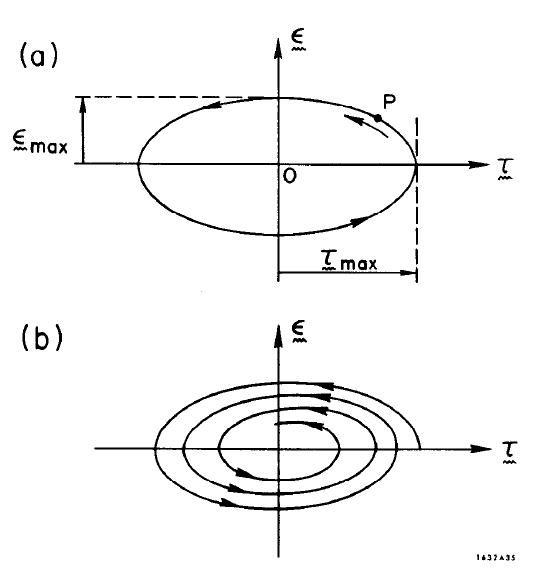
\includegraphics[width=0.6\linewidth]{./Figuras/fig35.jpeg}
	\caption{Phase diagram for energy oscillations. (a) Without damping. (b) With damping. (The damping rate is very much exaggerated).}
	\label{fig:fig35}
\end{figure}

If the scales are chosen so that the ellipse becomes a circle, the reference point rotates at the constant angular frequency $\Omega$. With damping, the size of the ellipse decreases slowly and the phase trajectory is a slow inward spiral as indicated crudely in \autoref{fig:fig35}(b). The phase diagram also makes transparent why the damping depends on $dU_{rad}/dE$. If this derivative is positive, the electron is losing a little extra amount of energy while on the upper half of the ellipse, and gaining a little extra energy while on the lower half. So it is always “drifting” toward the axis of $\tau$ and the oscillation amplitude is decreasing -- in proportion to $dU_{rad}/dE$.

According to our solution, the energy oscillations of all electrons should ultimately be completely damped out and they should all end up on top of the synchronous electron. But we have not yet taken into account the excitation of the oscillations by the quantum effects which “shake up” the oscillations and prevent them ever from going completely to zero. (They are considered in the next part). Under stationary conditions any stored electron will typically be found with some residual oscillation amplitude in which there is a balance between the excitation and the damping. Since both of these processes are slow we may think of the energy oscillation during any brief time as being described by a fixed phase ellipse such as the one in \autoref{fig:fig34}(a).

I should also remind you that the energy oscillations relate not only to the longitudinal oscillations (in $z$ or $\tau$) of the electrons in a bunch but have also a lateral component. According to Eq. \eqref{eq:3.3} an energy deviation $\epsilon$ results in a radical displacement $x_\epsilon$ which is proportional to $\epsilon$ and in phase with it. So the component $x_\epsilon$ of the total horizontal displacement oscillates in synchronism with the energy oscillations. Generally, this transverse manifestation of the energy oscillations has (under stationary conditions) about the same amplitude as the betatron oscillations.

    \subsection{Large Oscillations; Energy Aperture}\label{sec:3.6}

A storage ring guide field can usually accept only a small range of energies -- typically
 only a few percent of the nominal energy -- and the magnetic focusing forces are usually reasonably linear over the whole energy range. Even much smaller energy deviations however, may correspond to rather large oscillations of the time displacement $\tau$. I mean by ``large'' oscillations those for which $V(\tau)$ departs significantly from a linear dependence on $\tau$.
 Such large amplitudes may typically occur when the peak rf voltage is not very much larger than the radiation loss (as is usually the case at very high energies) or when the rf harmonic number
$k$ is very large. We should take at least a brief look at the large amplitude oscillations  because they are generally responsible for determining the energy “aperture” -- or “acceptance”
 -- of a ring. Please keep in mind however, that although we shall be dealing with ``large'' time displacements -- which may encompass a major fraction of an rf period - the maximum energy deviations will still be ``small'', a very small fraction of the energy itself.\\
We may begin with the two basic results of the preceding section, Eqs.~\eqref{eq:3.32} and \eqref{eq:3.34}. As before, we replace $U_{\text{rad}}$ by $U_0 + D\epsilon$, since the energy deviations remain small. But we must retain $V(\tau)$ without any simplification. We get for
Eq.~\eqref{eq:3.34}
\begin{align}
	\dfrac{d\epsilon}{dt} = \dfrac{eV(\tau)-U_0}{T_0}-\dfrac{D\epsilon}{T_0}.
\end{align}
If we now express both $\epsilon$ and its time derivative in terms of $\tau$ by using Eq.~\eqref{eq:3.32} we get the following equation.
\begin{align}\label{eq:3.49}
	\dfrac{d^2\tau}{dt^2} = -\dfrac{\alpha}{E_0 T_0} \left\lbrace eV(\tau) - U_0 \right\rbrace - \dfrac{D}{T_0} \dfrac{d\tau}{dt}.
\end{align}
This equation describes the variation of $\tau$ for all amplitudes.\\
I now ask you to look at another equation which is probably familiar to you:
\begin{align}\label{eq:3.50}
	m\dfrac{d^2x}{dt^2} = F(x) - \mu \dfrac{dx}{dt}.
\end{align}
It represents the motion in one dimension, $x$, of a particle of mass $m$, which
moves in a conservative force field $F(x)$, and suffers a frictional drag force proportional
 to its speed. We can understand Eq.~\eqref{eq:3.49} by making a direct comparison between it and Eq.~\eqref{eq:3.50}. The motion in $\epsilon$ is exactly like the motion of a particle of unit mass which moves in the conservative force field
\begin{align}\label{eq:3.51}
	F(\tau) = - \dfrac{\alpha}{E_0 T_0} \left\lbrace eV(\tau) - U_0 \right\rbrace.
\end{align}
and which is subject to a frictional drag proportional to the velocity with a drag coefficient
 $D/T_0$.\\
 The motion in $\tau$ can, in general, only be evaluated by a numerical computation. We can however, get a good heuristic idea of the motion by considering first what happens if the friction term is zero. It is small anyway and can be taken into account later as a perturbation.
 We wish to study the motion
\begin{align}
	m\dfrac{d^2x}{dt^2} = F(x)
\end{align}
with $F(\tau)$, given by Eq.~\eqref{eq:3.51}. As you know such an equation is often handled by
defining a ``potential energy'' function $\Phi(\tau)$ which is the negative of the integral
 of the force. Let's define
\begin{align} \label{eq:3.53}
	\Phi(\tau) = \dfrac{\alpha}{E_0 T_0} \int_0^\tau \left\lbrace eV(\tau) - U_0 \right\rbrace d\tau.
\end{align}
We can then analyze the motion by evoking the principle of conservation of ``energy''. At each instant the sum of the ``potential energy'' $\Phi(\tau)$ and the ``kinetic energy'' -- here $\frac{1}{2} (d\tau/dt)^2$ -- must be a constant, the ``total energy''. The total energy is
also the maximum $\Phi_0$ that can be reached by $\Phi(\tau)$ -- which will occur when $d\tau/dt$
is zero -- so we may write that
\begin{align}\label{eq:3.54}
	\dfrac{1}{2}\left(\dfrac{d\tau}{dt}\right)^2 = \Phi_0 - \Phi(\tau).
\end{align}
Suppose that the energy gain function $eV(\tau)$ has the form shown in Fig.~\ref{fig:fig36}(a) and that the synchronous energy gain $U_0$ is as shown there. Then $\Phi(\tau)$ will be as drawn in part (b) of the figure. The form shown is quite typical.  Notice that there is a general downward trend of $\Phi(\tau)$ with an average slope of $-U_0$. This must occur because the rf accelerating fields must integrate to zero over each complete cycle (at least over each complete cycle of the lowest frequency present).\\
You can now visualize the nature of the time displacement oscillations. The motion is like that of a point particle (an ``electron'') which slides around ``on'' the hilly surface represented by $\Phi(\tau)$ -- where you must of course, think of $\tau$ as a horizontal spatial coordinate. First, there is a potential minimum at $\tau = 0$. If you place an electron there it remains stationary; it is a ``synchronous electron''\footnote{There are of course, stationary points at each potential minimum and these correspond to the synchronous electrons at the centers of other bunches (so long as $\tau < T_0$)}. It however, you place an electron at $\tau_1$ -- so that it is at point $A$ on the hill -- it will slide down the hill and coast up the other side to point $B$. Both $A$ and $B$ are at the same height $\Phi_0 = \Phi(\tau_A)$. At $\tau_A$ and $\tau_B$
 the ``kinetic energy'' will be zero. The kinetic energy will reach its maximum value as the electron passes $\tau = 0$. At each $\tau$ the kinetic energy is given by Eq.~\eqref{eq:3.54} and from it we can obtain the ``velocity'' at each $\tau$:
\begin{align}
	\dfrac{d\tau}{dt} = \pm \sqrt{2} \left[ \Phi_0 - \Phi(\tau) \right]^{1/2}.
\end{align}
Remember, now, that according to Eq.~\eqref{eq:3.32} the ``velocity'' is
\begin{align*}
	\dfrac{d\tau}{dt} = - \alpha \dfrac{\epsilon}{E_0},
\end{align*}
so that the energy deviation (of the real electron) at each $\tau$ is given by
\begin{align}\label{eq:3.56}
	\dfrac{\epsilon(\tau)}{E_0} = \mp \dfrac{\sqrt{2}}{\alpha} \left[ \Phi_0 - \Phi(\tau) \right]^{1/2}.
\end{align}

\begin{figure}[!htb]
	\centering
	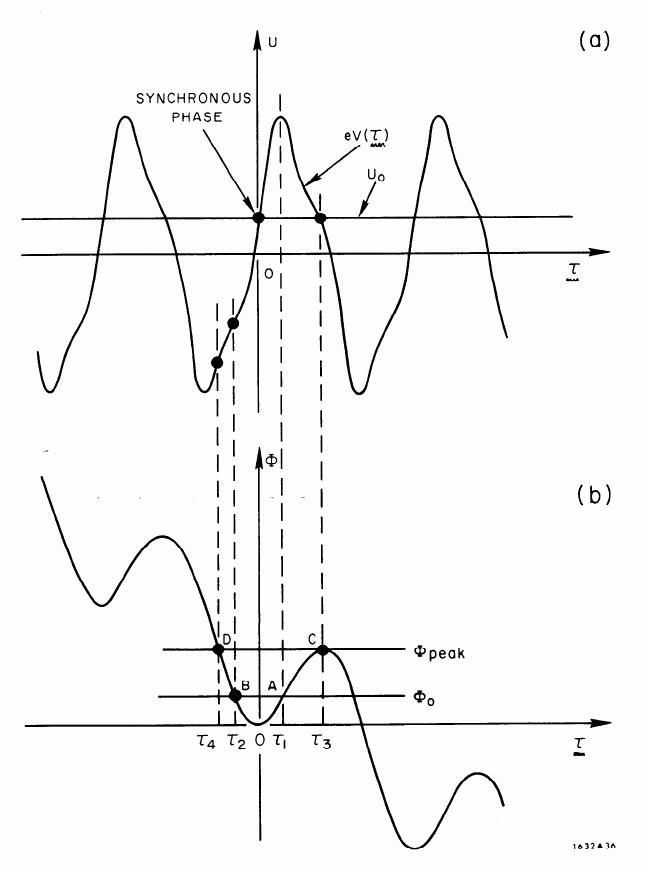
\includegraphics[width=0.8\linewidth]{./Figuras/fig36.jpeg}
	\caption{(a) The rf accelerating function $eV(\tau)$, and (b) the effective potential energy function $\Phi(\tau)$.}
	\label{fig:fig36}
\end{figure}

you can easily see that if you plot a phase diagram -- $\epsilon$ versus $\tau$ -- you will get
a more-or-less elliptical curve much like the curve a drawn in Fig.~\ref{fig:fig37}. You must only use-your common sense to choose the proper sign for the square root on each half cycle.

\begin{figure}[!htb]
	\centering
	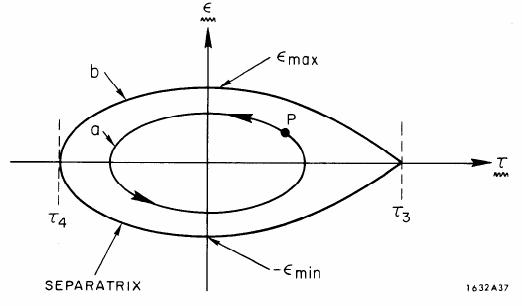
\includegraphics[width=0.8\linewidth]{./Figuras/fig37.jpeg}
	\caption{Phase diagram for large oscillations. Bounded energy oscillations occur only inside of the separatrix.}
	\label{fig:fig37}
\end{figure}

Also you can see what would happen if you were now to include the friction term -- the radiation
 damping. During each oscillation cycle a small amount of energy would be lost in a resulting decrease of the total ``energy'' (You could even estimate this loss by, say, approximating the motion by a sinusoid).\\
It should also be apparent that there will be a maximum amplitude of a stable (periodic) oscillation of $\tau$. It occurs when the electron can just reach the peak of the hill at $\tau_3$ -- corresponding to the point $C$ in Fig.\ref{fig:fig36}(b) - where $\Phi(\tau)$ takes on the value $\Phi_\text{max}$. An electron with any larger amplitude will sail on over the peak
and on into the next valley where it will have so much ``kinetic energy'' that it will keep on going forever -- until it is lost from the storage ring.\\
The maximum stable oscillation goes back and forth between the points $C$ and $D$. Notice that the point $C$ is also where $eV(\tau)$ is again equal to $U_0$. (To the left of $C$ the real electron always gains energy and may have some hope of returning to the origin of $\tau$). The other extreme of the oscillation at point $D$ has no special quality except that $\Phi(\tau)$ is again equal to $\Phi_\text{max}$, the value at $C$. The phase diagram of the extreme oscillation
 is a little peculiar, since both the velocity and the acceleration go to zero at $C$ but not at $D$.  The electron ``lingers'' at $C$ - in the ideal case for an infinite time! As a result the phase diagram will have a ``corner'' as shown by the curve (b) of Fig.~\ref{fig:fig37}. This special curve is called the separatrix, because it separates the stable oscillations from the unstable trajectories. An electron injected into a storage ring with a certain energy deviation $\epsilon$ and time displacement $\tau$ corresponding to the point $P$ in Fig.~\ref{fig:fig37} will circulate on a more-or-less elliptical closed curve (neglecting damping). If an electron is injected at a point outside the separatrix it is ``lost''.\\
 You can now see how the rf system can determine the energy aperture of a storage ring. Energy deviations larger than $\pm\epsilon_\text{max}$ -- of Fig.~\ref{fig:fig37} -- cannot be held in the storage ring. Electrons may be lost at smaller energy deviations if the lateral displacements
 $x_\epsilon$ associated with $\epsilon$ cause the electron to collide with some physical obstruction that limits the radial aperture. Normally, however, the rf limitation sets in first
 and the energy aperture is $\pm\epsilon_\text{peak}$. From Eq.~\eqref{eq:3.56},
\begin{align}
	\dfrac{\epsilon_{\max}}{E_0} = \dfrac{1}{\alpha} (2 \Phi_{\max})^{1/2}.
\end{align}
For the special case of an rf voltage function that is a pure sinusoid -- as described by Eq.~\eqref{eq:3.36} -- it is possible to calculate $\Phi(\tau)$ using Eq.~\eqref{eq:3.53},
\begin{align}\label{eq:Phi_sine}
	\Phi(\tau) = \dfrac{\alpha U_0}{2\pi k E_0} \left\lbrace \sqrt{q^2-1} - q \cos [\omega_{\text{rf}}(\tau - \tau_0)] - \omega_{\text{rf}} \tau \right\rbrace,
\end{align}
in which
\begin{align} \label{eq:3.60}
q = e\hat{V}/U_0
\end{align}
is the overvoltage -- namely the ratio of the peak rf voltage to the minimum voltage required to store a synchronous electron. Notice that, from Fig.~\ref{fig:fig36}, $\Phi_{\max}$ happens the first time $\Phi'(\tau^*) = 0$ for $\tau^* > 0$. More precisely, we have the next point for which $\sin[\omega_{\text{rf}}(\tau^*-\tau_0)]$ assumes the same value as $\sin[\omega_{\text{rf}}(-\tau_0)]$, that is
\begin{align*}
	& \omega_{\text{rf}}(\tau^* - \tau_0) = \pi - \omega_{\text{rf}}(-\tau_0) \\
    \Rightarrow \, & \tau^* = \dfrac{\pi}{\omega_{\text{rf}}} + 2\tau_0.
\end{align*}

Plugging this result in Eq.~\eqref{eq:Phi_sine}, results in
\begin{align} \label{eq:3.58}
	\Phi_{\max} = \dfrac{\alpha U_0}{2\pi k E_0} F(q),
\end{align}
where
\begin{align}
	F(q) = 2\left\lbrace \sqrt{q^2 - 1} - \arccos(1/q) \right\rbrace.
\end{align}

The energy aperture $\epsilon_{\max}$ for this case is then given by
\begin{align}
	\left(\dfrac{\epsilon_{\max}}{E_0}\right)^2 = \dfrac{U_0}{\pi \alpha k E_0} F(q).
\end{align}
The aperture function $F(q)$ is plotted in Fig.~\ref{fig:fig38}. Notice that for large $q$
\begin{align}
	F(q) \to 2q - \pi.
\end{align}

\begin{figure}[!htb]
	\centering
	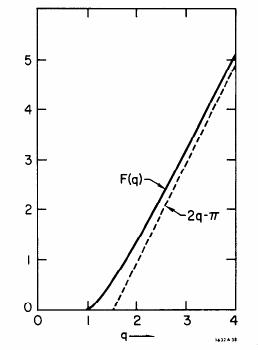
\includegraphics[width=0.5\linewidth]{./Figuras/fig38.jpeg}
	\caption{The energy aperture function F(q).}
	\label{fig:fig38}
\end{figure}

Finally if you think about what happens if you start an electron outside of the energy aperture
 -- say at points above the point D on the curve of $\Phi(\tau)$ in Fig.~\ref{fig:fig36}(b)
and figure out what their phase trajectories will be you will see that they become curves like the ones drawn in Fig.~\ref{fig:fig39}. Three successive separatrices are shown and several examples of unstable trajectories. Again you see that an electron once outside a stable region will -- barring a fortunate accident -- stay outside forever.

\begin{figure}[!htb]
	\centering
	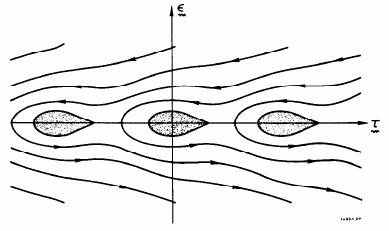
\includegraphics[width=0.8\linewidth]{./Figuras/fig39.jpeg}
	\caption{Phase trajectories for electrons not captured in a bunch (a qualitative sketch).}
	\label{fig:fig39}
\end{figure}


\chapter{Radiation Damping} \label{ch:4}
    \section{Energy loss}\label{sec:4.1}

A relativistic electron which is accelerated in a macroscopic force field will radiate electromagnetic energy at a rate which is proportional to the square of the accelerating
 force. The rate depends on the angle between the force and the electrons velocity and is larger by the factor $\gamma^2 = (E/mc^2)^2$ when the force is perpendicular to the velocity than when the force is parallel to the velocity. In a storage ring the typical longitudinal forces (from the accelerating system) are much smaller than the typical transverse magnetic forces and $\gamma^2$ is a large number indeed, so we need consider only the radiation effects that accompany the magnetic forces.\\
Let $P_\gamma$ stand for the rate of loss of energy by radiation; it may be written\footnote{I shall assume that you are familiar with the classical theory of electromagnetic radiation by relativistic electrons (see e.g., Ref.~\cite{10}) and will only review briefly the results needed for our purposes.}
\begin{align}
	P_\gamma &= \dfrac{2}{3} \dfrac{r_e}{m c} \gamma^2 F_\perp^2 \nonumber \\
    	&= \dfrac{2}{3} \dfrac{r_e c}{(m c^2)^3} E^2 F_\perp^2,
\end{align}
where $m$ is the rest mass of the electron, $r_e = \dfrac{e^2}{m_e c^2}$ is the classical electron radius, and $F_\perp$ is the magnetic force on the electron.

\begin{proof}
We will begin with the expression of the electric field produced by an accelerated electron (considering the velocity still small compared to the velocity of light) at a point of coordinates $(r,\phi,\theta)$, with the electron on the origin; this expression is

\begin{align*}
E = \dfrac{e\dot{v}\sin \theta}{c^2 r}.
\end{align*}
In order to calculate the rate of energy radiated by the electron, we must obtain the expression for the poynting vector $|\mathbf{S}| = (c/4\pi)E^2$ and integrate it over the area $dA$ related to the solid angle $d\Omega$ by $dA = r^2d\Omega = r^2\sin\theta d\theta d\phi$

\begin{align*}
P = \int_{0}^{2\pi}\int_{0}^{\pi}\dfrac{cE^2}{4\pi}r^2\sin\theta d\theta d\phi = \dfrac{2}{3}\dfrac{e^2a^{2}}{c^3}
\end{align*}
where $a$ is the acceleration of the particle. With Newton second law we rewrite the former expression in a convenient manner

\begin{align*}
P = \dfrac{2}{3}\dfrac{e^2}{m^2c^3} \left(\dfrac{d\mathbf{p}}{dt}\cdot\dfrac{d\mathbf{p}}{dt}\right)
\end{align*}

Since we wish to approach the relativistic limit, we must use covariant expressions to generalize our results and the straighforward covariant expression of radiation power is simply

\begin{align*}
P = -\dfrac{2}{3}\dfrac{e^2}{c^3} \dfrac{1}{m^2} \left(\dfrac{d{p_\mu}}{d\tau}\dfrac{dp^\mu}{d\tau}\right),
\end{align*}

where $d\tau = \gamma^{-1}dt$ is the proper time and the Minkowski metric is $g_{\mu \nu} = (+ - - -)$. Performing the scalar product of these quadrivectors we obtain

\begin{align*}
-\dfrac{d{p_\mu}}{d\tau}\dfrac{dp^\mu}{d\tau} = \left(\dfrac{d\mathbf{p}}{d\tau}\right)^2 - \frac{1}{c^2}\left(\dfrac{dE}{d\tau}\right)^2 = \left(\dfrac{d\mathbf{p}}{d\tau}\right)^2 - \beta^2\left(\dfrac{dp}{d\tau}\right)^2
\end{align*}

Consider that there is no transversal momentum (which is the case of an electron on a circular orbit), then $\boldsymbol{{p}} = \boldsymbol{p}_\parallel$ or equivalently $\boldsymbol{\beta} = \boldsymbol{\beta_\parallel}$. Although, there is a longitudinal and a transversal force components, therefore
 there is such components for the derivative of momentum. The parallel acceleration is related to the parallel force by $mc\gamma^3\boldsymbol{\dot{\beta}}_\parallel = \dfrac{d\mathbf{p}_\parallel}{dt} = \mathbf{F}_\parallel$ and the transverse acceleration can be obtained from the Lorentz force by
 $mc \gamma\boldsymbol{\dot{\beta}}_\perp = \dfrac{d\boldsymbol{p}_{\perp}}{dt} = ec\boldsymbol{{\beta}} \times \mathbf{B} = \mathbf{F}_\perp$. Obviously $\mathbf{F}_\parallel \cdot \mathbf{F}_\perp = 0$, thus

 \begin{align*}
 -\dfrac{d{p_\mu}}{d\tau}\dfrac{dp^\mu}{d\tau} = (1- \beta^2)\left(\dfrac{dp_\parallel}{d\tau}\right)^2 + \left(\dfrac{dp_\perp}{d\tau}\right)^2,
 \end{align*}

 using that $1-\beta^2 = \gamma^{-2}$ and $d\tau = \gamma^{-1}dt$, we obtain two components for the radiation power

\begin{align*}
P_\parallel &=   \dfrac{2}{3}\dfrac{e^2}{m^2c^3}F_\parallel^2 \\
P_\perp &=   \dfrac{2}{3}\dfrac{e^2 \gamma^2}{m^2c^3}F_\perp^2 .
\end{align*}

Since we know that $E = \gamma mc^2$, becomes explicit that the radiation power for parallel acceleration does not depends on particle energy, while the transverse radiation power does. That means that applying the same accelerating force on the particle, we will obtain much more radiation power if the acceleration
is transverse to the propagation of the charged particle than if it is longitudinal.
\end{proof}

It will be convenient to define the constant
\begin{align} \label{eq:4.2}
	C_\gamma = \dfrac{4 \pi}{3} \dfrac{r_e}{(m c^2)^3} = 8.85 \times 10^{-5}\, \text{m-GeV}^{-3}.
\end{align}
Then since $F_\perp = ecB$, the radiated power is
\begin{align} \label{eq:4.3}
	P_\gamma = \dfrac{e^2 c^3}{2 \pi} C_\gamma E^2 B^2.
\end{align}
This instantaneous power is proportional to the square of both the energy and the local magnetic field strength. It is sometimes useful to express the magnetic force in terms of the local radius of curvature $\rho$ of the trajectory; then
\begin{align} \label{eq:4.4}
	P_\gamma = \dfrac{c C_\gamma}{2 \pi}\dfrac{E^4}{\rho^2}.
\end{align}
An electron circulating on the design orbit has the nominal energy $E_0$ and moves on the radius $\rho = 1/G$ - see Section~\ref{sec:2.2}. To find the energy $U_0$ radiated in one revolution
 we must integrate $P_\gamma$ with respect to time once around the ring. Since $dt = ds/c$,
\begin{align} \label{eq:4.7}
	U_0 = \dfrac{C_\gamma E_0^4}{2 \pi} \oint G^2(s) ds.
\end{align}
For an isomagnetic guide field\footnote{See Section~\ref{sec:2.2}.} $G = G_0 = 1/\rho_0$ along the curved parts of length $2 \pi \rho_0$ and zero elsewhere, so
\begin{align} \label{eq:4.8}
	U_0 = \dfrac{C_\gamma E_0^4}{\rho_0}.
\end{align}
For a fixed radius $\rho_0$, the energy radiated per turn varies as the fourth power of the electron energy. A 1 GeV electron moving on a 5 meter radius looses 17 keV each revolution.\\
The average power radiated is $U_0/T_0$ where $T_0= L/c$ is the time elapsed during one revolution. For the general guide field
\begin{align} \label{eq:4.9}
	\mean{P_\gamma} = \dfrac{cC_\gamma}{2\pi} E_0^4 \mean{G^2}.
\end{align}
And for an isomagnetic ring,
\begin{align} \label{eq:4.10}
	\mean{P_\gamma} = \dfrac{c C_\gamma E_0^4}{\rho_0 L}, && \text{(isomag.).}
\end{align}
An electron that is not on the ideal orbit radiates at a different rate. Consider first an electron that has the nominal energy $E_0$. but is circulating with a betatron oscillation. It's rate of radiation will be different from an electron moving on the design orbit only because it moves through a slightly different magnetic field - due to its betatron displacement. But at each azimuth its displacement is equally often positive or negative. And we have assumed that the fields have only a linear variation with displacement. So -- to first order in the betatron amplitude the radiated power averaged -- over a betatron cycle is the same as that of an electron on the design orbit.\\
The same is not true of an electron with an energy different from $E_0$. That
case will be analyzed in the next section.
For ultra-relativistic electrons the radiation is emitted primarily along the direction of motion. Most of the radiation is emitted within the angle $1/\gamma$. The radiation reaction force -- and therefore, the accompanying momentum change -- is exactly opposite to the direction
 of motion\footnote{Neglecting quantum effects; see Section~\ref{sec:5.1}}. The only effect of the radiation is then to decrease the energy of the electron without changing its direction
 of motion.

    \section{Damping of the Energy Oscillations}\label{sec:4.2}

In Section~\ref{sec:3.5} we saw that small energy oscillations were damped at a rate proportional
 to the change of the radiation loss with energy. From Eqs. \eqref{eq:2.43} and \eqref{eq:3.24} the damping coefficient $\alpha_\epsilon$ is
\begin{align}
	\alpha_\epsilon = \dfrac{D}{2 T_0} = \dfrac{1}{2 T_0} \left( \dfrac{d U_\text{rad}}{d E}, \right)
\end{align}
where $U_\text{rad}$ is the energy loss per revolution. When the energy of an electron deviates from the nominal energy $E_0$, the energy radiated in one revolution changes in part because of the energy change, in part because the electron travels in a different magnetic field and in part because its path length is different. Let’s look at how $dU_\text{rad}/dE$ may be evaluated.\\
We have already seen that a betatron oscillation does not, to first order, change the average power radiated. So to get $U_\text{rad}$ at any energy we must merely integrate the $P_\gamma$ of Eq.~\eqref{eq:4.3} with respect to time around one complete off-energy closed orbit. It will, however, be convenient to change the variable of integration to $s$. Then,
\begin{align}
	U_\text{rad} = \oint P_\gamma dt = \oint P_\gamma \dfrac{dt}{ds} ds.
\end{align}
We have earlier evaluated $dt/ds$, see Eq.~\eqref{eq:2.15}:
\begin{align*}
	\dfrac{dt}{ds} = \dfrac{1}{c} \left( 1 + \dfrac{x}{\rho_s} \right),
\end{align*}
where $x$ is the displacement from the design orbit and $\rho_s(s)$ is the radius of curvature of the design orbit. Since we are now interested in the energy loss on an off-energy closed orbit we should take $x = \eta \epsilon/E_0$, where $\epsilon = E - E_0$. and $\eta(s)$ is
the off-energy function. See Eq.~\eqref{eq:2.28}. Then
\begin{align}
	U_\text{rad} = \dfrac{1}{c} \oint \left( 1 + \dfrac{\eta}{\rho} \dfrac{\epsilon}{E_0} \right) P_\gamma ds.
\end{align}
We have already looked at this integral for $\epsilon = 0$; it is just $U_0$. So let’s differentiate now, evaluating the derivative at $\epsilon = 0$.
\begin{align} \label{eq:4.14}
	\dfrac{U_\text{rad}}{dE} = \dfrac{1}{c} \oint \left\lbrace \dfrac{dP_\gamma}{dE} + \dfrac{\eta}{\rho} \dfrac{P_\gamma}{E} \right\rbrace_0 ds,
\end{align}
where the subscript ``0'' on the curly brackets means that all quantities in the integrand are to be evaluated on the design orbit, and at the energy $E_0$. From Eq.~\eqref{eq:4.3}, $P_\gamma$ is proportional to the product $E^2 B^2$ -- and remember that when $E$ changes, the orbit moves to a different location so that $B$ also changes. We may then write that
\begin{align*}
	\dfrac{dP_\gamma}{dE} = 2 \dfrac{P_\gamma}{E_0} + 2 \dfrac{P_\gamma}{B_0} \dfrac{dB}{dE}.
\end{align*}
But
\begin{align*}
	\dfrac{dB}{dE} = \dfrac{dx}{dE} \dfrac{dB}{dx} = \dfrac{\eta}{E_0} \dfrac{dB}{dx},
\end{align*}
where $dB/dx$ is a property of the guide field. Putting these last two together and into Eq.~\eqref{eq:4.14}
\begin{align*}
	\dfrac{dU_\text{rad}}{dE} = \dfrac{1}{c} \oint \left\lbrace 2 \dfrac{P_\gamma}{E} + 2 \dfrac{P_\gamma}{B} \dfrac{\eta}{E_0} \dfrac{dB}{dx} + \dfrac{P_\gamma}{E} \frac{\eta}{\rho}  \right\rbrace_0 ds.
\end{align*}
The integral
 of the first
 term yields just $2U_0/E_0$ so our result for the variation of the radiated energy is
\begin{align}
	\dfrac{dU_\text{rad}}{dE} = \dfrac{U_0}{E_0} \left[ 2 + \dfrac{1}{cU_0} \oint \left\lbrace \eta P_\gamma \left( \dfrac{1}{\rho} + \dfrac{2}{B} \dfrac{dB}{dx} \right) \right\rbrace_0 ds \right]
\end{align}
We may now write for the damping constant:
\begin{align}\label{eq:4.16}
\alpha_\epsilon = \dfrac{1}{2 T_0} \dfrac{dU_\text{rad}}{dE} = \dfrac{U_0}{2 T_0 E_0} (2 + \mathscr{D}),
\end{align}
with
\begin{align}
	\mathscr{D} = \dfrac{1}{c U_0} \oint \eta P_\gamma \left\lbrace \dfrac{1}{\rho} + \dfrac{2}{B} \dfrac{dB}{dx} \right\rbrace_0 ds.
\end{align}

Taking $P_\gamma$ and $U_0$. from Eqs. \eqref{eq:4.3} and \eqref{eq:4.8} and expressing
 $B$ and $dB/dx$ in terms of $G(s)$ and $K_1(s)$ as defined in Section \ref{sec:2.2}, we may rewrite $\mathscr{D}$ as
\begin{align} \label{eq:4.18}
	\mathscr{D} = \dfrac{\oint \eta G (G^2 + 2K_1)ds}{\oint G^2 ds}.
\end{align}
This form makes clearer the fact that $\mathscr{D}$ is just a number which is a property of
the total guide field configuration -- obtained from integrations around the ring of expressions
 involving only the guide field functions $G$, $K_1$, and $\eta$. The number $\mathscr{D}$ is typically a positive number quite a bit smaller than 1.\\
Equation \eqref{eq:4.16} has a nice physical interpretation. Since $\mathscr{D}$ is usually small
we have the approximate relation:
\begin{align}
	\alpha_\epsilon \approx \dfrac{U_0}{E_0 T_0} = \dfrac{\mean{P_\gamma}}{E_0},
\end{align}
where $\mean{P_\gamma}$ is the average rate of energy loss. The damping time constant for energy oscillations -- which is the inverse of $\alpha_\epsilon$ -- is just the time it takes an electron to radiate away its total energy!\\
The expression above for $\mathscr{D}$ becomes simpler if the guide field is isomagnetic. Then $G(s)$ is either zero or equal to some constant in the magnets and the integrals extend only over the magnets. Equation \eqref{eq:4.18} becomes
\begin{align} \label{eq:4.20}
	\mathscr{D} = \dfrac{1}{2\pi}\oint_{\text{Mag}}\eta(s)\left\lbrace G_0^2 + 2K_1(s) \right\rbrace ds. && \text{(isomag)}
\end{align}
If the guide field is also ``separated function'' the magnets have no gradients and
\begin{align}\label{eq:4.17}
	\mathscr{D} = \dfrac{G_0^2}{2\pi}\oint_{\text{Mag}}\eta(s) ds. && \left(\begin{tabular}{l}
\text{isomag} \\
\text{sep. func.}
\end{tabular}\right)
\end{align}
The integral is familiar; it appeared earlier when we calculated the momentum compaction $\alpha$ for an isomagnetic guide field. Using Eqs. \eqref{eq:3.13} and \eqref{eq:3.14},
\begin{align}
	\mathscr{D} = G_0 \mean{\eta}_\text{Mag} = \dfrac{\alpha L}{2 \pi \rho_0} && \left(\begin{tabular}{l}
\text{isomag} \\
\text{sep. func.}
\end{tabular}\right)
\end{align}
For this type of ring, the number $\mathscr{D}$ is just the momentum compaction $\alpha$ increased by the ratio of the perimeter of the ring $L$ to the magnetic perimeter $2\pi\rho_0$. Typical values for these parameters of a ring might be:
\begin{align*}
	\alpha \approx 0.05; && L/(2\pi\rho_0)\approx 3; && \mathscr{D} \approx 0.15.
\end{align*}
Recapitulating, for energy oscillations in an isomagnetic, separated function guide field, the damping coefficient for energy oscillations is
\begin{align}
	\alpha_\epsilon = \dfrac{\mean{P_\gamma}}{2E_0}\left( 2 + \dfrac{\alpha L}{2 \pi \rho_0} \right). && \left(\begin{tabular}{l}
\text{isomag} \\
\text{sep. func.}
\end{tabular}\right)
\end{align}

    \section{Damping of Betatron Oscillations}\label{sec:4.3}
It is now time to take a look at the so-called radiation damping of the betatron oscillations. I shall give here only an approximate treatment, but using a method which can -- with only a bit of tedious algebra -- be extended to an exact calculation. The exact result is, in any case, obtained more easily by a general theorem that will be discussed in the next section.\\
Let's look first at the vertical betatron oscillations (the notation will be the one used in Part II). I shall approximate the motion by ignoring the variation of $\beta$ with $s$, then I may write (see Section \ref{sec:2.8})
\begin{align}
	z = A \cos(\varphi), && z' = \dfrac{A}{\beta}\sin(\varphi),
\end{align}
where $\varphi$ is $s/\beta$. The amplitude $A$ of the oscillations can be obtained from $z$ and
$z'$ at any instant by
\begin{align}
	A^2 = z^2 + (\beta z')^2
\end{align}
Suppose we are looking at an electron of energy $E_0$ -- which is then oscillating vertically
 about the design orbit. In any element of azimuth $\delta s$ the electron will lose by radiation
 the small amount of energy $\delta E$. Its momentum vector $\bm{p}$ will be changed by $\delta \bm{p}$ and, as was remarked earlier $\delta \bm{p}$ is parallel (and opposite) to $\bm{p}$,so $|\delta \bm{p}| = \delta E/c$. See Fig.~\ref{fig:fig40}(a). The radiation loss does not change either the displacement or the slope of the trajectory; and so the amplitude $A$ is unchanged
by the radiation (there is a small effect due to the fact that the effective focusing forces and, therefore, also $\beta$ are changed with a change of energy but this so-called "adiabatic" damping effect is of second order and can, anyway, be neglected since the energy is not changing on the average when the rf acceleration is also taken into account).

\begin{figure}[!htb]
	\centering
	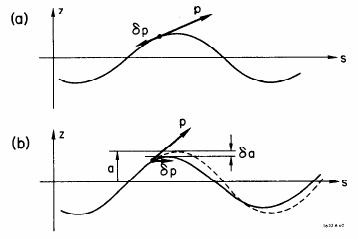
\includegraphics[width=0.8\linewidth]{./Figuras/fig40.jpeg}
	\caption{Effect of an energy change on the vertical betatron oscillations: (a) for radiation loss, (b) for rf acceleration.}
	\label{fig:fig40}
\end{figure}

Notice now, that the effect of the rf accelerating force is quite different. This force is, on the average, parallel to the design orbit. Then the momentum increment $\delta\bm{p}$ received in the azimuthal element $\delta s$ is no longer exactly parallel to $\bm{p}$. See Fig. \ref{fig:fig40}(b). Let's write $p_\perp$, for the component of $\bm{p}$ perpendicular to the design orbit; then, since the angles are small we may write
\begin{align}
	z' = \dfrac{p_\perp}{p}
\end{align}
Again, the accelerating force doesn't change $z$. But now it does change $z'$ which goes over to
\begin{align}
	z' = \dfrac{p_\perp}{p + \delta p} = \dfrac{p_\perp}{p} \left( 1 - \dfrac{\delta p}{p} \right) = z' \left( 1 - \dfrac{\delta p}{p} \right).
\end{align}
The change in z’ is
\begin{align}
	\delta z' = -z' \dfrac{\delta p}{p} = -z' \dfrac{\delta E}{E}.
\end{align}
There is a corresponding change in the amplitude $A$;
\begin{align}
	A \delta A = \beta^2 z' \delta z' = -(\beta z')^2 \dfrac{\delta E}{E}.
\end{align}
Now the phase of the oscillation at the arrival of the electron at the point $s$ is arbitrary
 (and all values between $0$ and $2\pi$ are equally probable) so we should inquire only about the average change in $A$. The average of $(z')^2$ is $A^2/2\beta^2$, so
\begin{align}
	A \mean{\delta A} = - \dfrac{A^2}{2} \dfrac{\delta E}{E_0}.
\end{align}
Suppose we now sum over all the elements of acceleration gain in one revolution. Since all of the $\delta E$ must add up to the radiation loss $U_0$, we find for the change $\Delta A$ that occurs in $A$ during one revolution (due to the rf acceleration):
\begin{align}
	\dfrac{\Delta A}{A} = - \dfrac{U_0}{2 E_0}.
\end{align}
Since $\Delta A$ in each revolution time $T_0$ is proportional to $A$, the motion is exponentially damped -- as $e^{-\alpha_z t}$ . That is,
\begin{align} \label{eq:4.31}
	\dfrac{1}{A} \dfrac{dA}{dt} = \dfrac{\Delta A}{A T_0} = - \dfrac{U_0}{2 E_0 T_0},
\end{align}
so the damping coefficient is
\begin{align}
	\alpha_z = \dfrac{U_0}{2 E_0 T_0} = \dfrac{\mean{P_\gamma}}{2 E_0}.
\end{align}
You can show that an exact calculation -- using the full-blown form for the vertical betatron oscillation -- yields the same result. Notice that the damping rate for the vertical oscillations
 is just $1/2$ the typical rate for the energy oscillations (when $\mathscr{D}$ is small); see Eq.~\eqref{eq:4.20}.\\
It is amusing to notice that the "radiation" damping does not occur in the radiation process, but rather in the process of energy gain from the rf system. One might question the appropriateness of the name "radiation damping". But on second thought, there would be no opportunity for damping by the rf fields if there were not the necessity to compensate for the energy loss by radiation. So the name "radiation damping" is not so bad.\\
Now let’s turn to the radiation effects on the radial betatron oscillations. You might at first,
 think that the radial betatron oscillations would be radiation damped in the, same way as the vertical ones. But there are additional complications so we shall have to treat them as a new problem. One new element arises from the change in the betatron displacement that occurs when there is an energy change. Remember that the total radial displacement $x$ is the sum of two parts: the displacement $x_\epsilon$ of the off-energy closed orbit, plus the betatron displacement $x_\beta$ with respect to the closed orbit,
\begin{align} \label{eq:4.33}
	x = x_\epsilon + x_\beta.
\end{align}
When the energy of an electron changes by $\delta E$, there is a change of $x_\epsilon$ by the
amount, see Eq.~\eqref{eq:2.28},
\begin{align}
	\delta x_\epsilon = \eta \dfrac{\delta E}{E_0}.
\end{align}
But since the position in space of the electron is not changed by a finite momentum impulse,
 the total $x$ does not change, so there must be a compensatory change in $x_\beta$. That is, from Eq.~\eqref{eq:4.33},
\begin{align*}
	\delta x = \delta x_\epsilon + \delta x_\beta = 0,
\end{align*}
from which
\begin{align} \label{eq:4.35}
	\delta x_\beta = -\delta x_\epsilon = -\eta \dfrac{\delta E}{E_0}.
\end{align}
When there is an energy change, the electron doesn't instantaneously move, but the reference
 axis of its oscillations does and the displacement with respect to that axis is therefore changed -- as is illustrated in Fig.~\ref{fig:fig41}.

\begin{figure}[!htb]
	\centering
	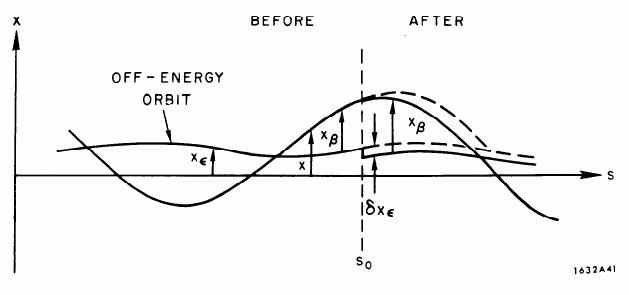
\includegraphics[width=0.8\linewidth]{./Figuras/fig41.jpeg}
	\caption{Effect of a sudden energy change at $s_0$ on the betatron displacement.}
	\label{fig:fig41}
\end{figure}
Something similar occurs for the betatron slope. Corresponding to Eq.~\eqref{eq:4.33} we must have
\begin{align}
	x' = x_\epsilon'+x_\beta'.
\end{align}
Only now, an elementary impulse may change the total $x'$ by some $\delta x'$ so we should
have for the change in the betatron slope
\begin{align}
	\delta x_\beta' = \delta x' - \delta x_\epsilon'.
\end{align}
Taking the derivative $x_\epsilon'$ from Eq.~\eqref{eq:2.28},
\begin{align} \label{eq:4.38}
	\delta x_\beta' = \delta x' - \eta' \dfrac{\delta E}{E_0}.
\end{align}
where $\eta'$ is, of course, $d\eta/ds$. Even if $\delta x'$ were zero, a change in the slope of $x_\epsilon$ the baseline of the oscillations -- would produce a change in the slope of the betatron oscillation.\\
Still an additional complication arises from the curvature of the reference orbit. The positive
 and negative halves of a betatron oscillation occur in equal intervals of $s$, but the electron
 travels a greater path length on the positive swing than on the negative swing - see Eq.~\eqref{eq:3.7}. Although the net effect on the path length is zero, over a complete oscillation, there is, in general, a different amount of energy lost by radiation during the two halves of an oscillation. And the amplitude of the oscillation is thereby affected.\\
Now let's apply these ideas to the radiation loss $\delta E$ in an azimuthal element $\delta s$.
 A precise calculation would proceed from the changes in $x$ and $x'$ found in Eqs. \eqref{eq:4.35} and \eqref{eq:4.38}. In keeping with the approximations made earlier in this
section, however, I am going to make the simplifying assumption that $\eta$ is a constant, so that $\eta' = 0$; and write the variation of $x_\beta$ with $s$ in the same form that I took for $z$; namely,
\begin{align}
	x_\beta = A \cos \varphi; && x_\beta' = \dfrac{A}{\beta} \sin \varphi.
\end{align}
This time we have that
\begin{align}
	A \delta A = x_\beta \delta x_\beta + \beta^2 x_\beta' \delta x_\beta',
\end{align}
and since only $\delta x_\beta$ is different from zero,
\begin{align} \label{eq:4.41}
	A \delta A = - x_\beta \eta \dfrac{\delta E}{E_0}
\end{align}
Again let's take the energy change $\delta E$ as the radiation loss in an azimuthal element $\delta s$. For the $z$-motion we assumed that the electron was always moving with zero radial displacement so the rate of radiation loss was the same (to first order in $z$) as the rate of energy loss on the design orbit. Things are different for the $x$-motion if the magnets have a field gradient. To simplify the discussion here I will restrict consideration to an isomagnetic
 and separated function guide field (see Section \ref{sec:2.2}). In a separated function machine the rate of radiation loss is independent of $x$ -- to first order\footnote{There is only a field gradient in the quadrupoles; where $B$ is proportional to $x$. Since the rate of radiation varies is $B^2$ there is no first order effect.}. I may then take that (for an electron of the nominal energy) the rate of radiation loss $P_\gamma(s)$ does not depend on $x$, but only on $s$.
The energy change in a path element is then
\begin{align}
	\delta E = P_\gamma \dfrac{\Delta \ell}{c}.
\end{align}
Taking for $\Delta \ell$ the expression in \eqref{eq:2.15},
\begin{align}
	\delta E = - P_\gamma \left( 1 + \dfrac{x_\beta}{\rho_s} \right) \dfrac{\Delta s}{c} .
\end{align}
Combining this result with Eq.~\eqref{eq:4.41} we have for the amplitude change,
\begin{align}
	A \delta A = x_\beta \eta P_\gamma \left( 1 + \dfrac{x_\beta}{\rho_s} \right) \dfrac{\Delta s}{c}
\end{align}
Again we are interested only in the expectation value of $\delta A$ -- the average over all
phase angles $\varphi$. The expectation value of $x$ is zero and of $x^2$ is $A^2/2$; we get that
\begin{align}
	\dfrac{\mean{\delta A}}{A} = \dfrac{\eta P_\gamma}{2 \rho_s} \dfrac{\Delta s}{cE_0}
\end{align}
Since I am assuming an isomagnetic guide field wherever $P_\gamma$ is different from zero $\rho = \rho_s = 1/G_0$ and we can easily sum up the effect at each $\Delta s$ to get the change $\Delta A$ in one complete revolution. The sum of all $P_\gamma s/c$ is just the energy loss $U_0$ in one complete turn. So we have for the effect of the radiation
\begin{align}
	\left( \dfrac{\Delta A}{A} \right)_\text{rad} = \dfrac{\eta}{2\rho_0}\dfrac{U_0}{E_0}.
\end{align}
Observe that the sign on the right hand side is positive. There is an increase of the amplitude
 due to the radiation!\\
Fortunately, this is only part of the story. We must also take into account the effect of the rf acceleration. For it however, there is no corresponding "path length" effect. Generally the rf cavities are located in places where $\rho = \infty$ ; but in any case, it is a property of such cavities that the energy gain is (to first order at least) independent of the betatron displacement. The calculation of the contribution from the rf acceleration goes exactly the same as for the vertical oscillations with the result shown in Eq.~\eqref{eq:4.31}. To get the total effect in one revolution we must add the contributions from the radiation loss and from the acceleration to get
\begin{align}
	\dfrac{\Delta A}{A} = - \left(1 - \dfrac{\eta}{\rho_0} \right) \dfrac{U_0}{2 E_0}.
\end{align}
which gives for the damping coefficient $\alpha_x$ of the radial oscillations
\begin{align}\label{eq:4.48}
	\alpha_x = - \left(1 - \dfrac{\eta}{\rho_0} \right) \dfrac{U_0}{2 E_0 T_0}.
\end{align}
A precise calculation for a separated function isomagnetic guide field gives exactly the same result, if we replace $\eta$ by $\mean{\eta}_\text{Mag}$, the mean value of $\eta(s)$ in the magnets. But recalling Eq.~\eqref{eq:3.14}, $\mean{\eta}_\text{Mag} = 2\pi L\alpha$ so
\begin{align} \label{eq:4.49}
	\alpha_x = - \left(1 - \dfrac{\alpha L}{2\pi\rho_0} \right) \dfrac{U_0}{2 E_0 T_0}. && \left(\begin{tabular}{l}
\text{isomag} \\
\text{sep. func.}
\end{tabular}\right)
\end{align}
Provided $\alpha L/2\pi\rho_0$ is less than 1 -- as it usually is -- the damping coefficient
 is positive and the radial oscillations are damped. But there is an "antidamping" effect of the radiation -- the term $\alpha L/2\pi\rho_0$ -- which counteracts somewhat the positive damping from the rf system. So long as the antidamping term is small no harm is done.
If you compare Eq.~\eqref{eq:4.49} with the results of the preceding section you will see that we may also write our result in terms of the parameter $\mathscr{D}$ defined there:
\begin{align}\label{eq:4.50}
	\alpha_x = (1-\mathscr{D}) \dfrac{U_0}{2E_0 T_0}. && (\text{general})
\end{align}
Although we have demonstrated this result only for a special kind of guide field (and with some approximations) Eq.~\eqref{eq:4.50}, it turns out, is exactly -- true for any guide field. That is, if we had in our treatment kept account of the effect of the variation of $\eta$ with $s$ we would have found that in place of $\eta/\rho_0$ in Eq.~\eqref{eq:4.48} we would have the complete expression for $\mathscr{D}$ in Eq.~\eqref{eq:4.17}. More will be said about this interesting "coincidence" in the next section.

    \section{Radiation Damping Rates}\label{sec:4.4}

Radiation damping effects have now been considered for all three degrees of freedom of an electron in a bunch: the two transverse betatron displacements $x_\beta$ and $z_\beta$ and the energy oscillations -- which show up also in associated oscillations of $\tau$ and $x_\epsilon$. Each of the three oscillation modes has a natural exponential decay with damping coefficients $\alpha_i$ (with $i = x, z$, or $\epsilon$) that can be conveniently expressed as
\begin{align}
	\alpha_i = J_i \alpha_0 = J_i \dfrac{\mean{P_\gamma}}{2 E_0},
\end{align}
with
\begin{align}
	J_x = 1 - \mathscr{D};&& J_z = 1;&& J_\epsilon = 2 + \mathscr{D}.
\end{align}
The damping time constants are just $1/\alpha_i$ so
\begin{align} \label{eq:4.53}
	\tau_i = \dfrac{2 E_0}{J_i \mean{P_\gamma}}.
\end{align}
For an isomagnetic storage ring $\mean{P_\gamma}$ may be taken from Eq.~\eqref{eq:4.10} then
\begin{align} \label{eq:4.54}
	\tau_i = \dfrac{2}{C_\gamma} \dfrac{L \rho_0}{J_i c E_0^3} && \text{(isomag.)},
\end{align}
where $C_\gamma$ is the constant defined in Eq.~\ref{eq:4.2}. In a given storage ring the damping
time constants vary as the inverse cube of the energy. The number $\mathscr{D}$ is a property
 of the guide field and may be evaluated from one of the equations \eqref{eq:2.10}, \eqref{eq:2.12}
 or \eqref{eq:2.13}). The numbers $J_i$ are known as the damping partition numbers since their sum is a constant:
\begin{align} \label{eq:4.55}
	\sum J_i = J_x + J_z + J_\epsilon = 4.
\end{align}
Although I have not actually proved this last result, it does indeed follow from detailed calculations for a general guide field. (See e.g., Ref. \cite{5}.) Such calculations are, however, not really necessary because Robinson has proved on very general grounds a theorem that yields Eq.~\eqref{eq:4.55} directly. The theorem required only that all of the fields acting on the particle are determined a priori and are not in any way influenced by the motion of the electron.
 These conditions apply if we consider only the prescribed magnetic and rf fields of a storage ring.\\
The damping rates for an individual electron -- and more importantly, for the coherent motion of a clump of them -- can be modified from the above numbers if additional forces are introduced
 that depend on the details of the electron motion. Such forces may, for example, come from image currents in the wall of the vacuum chamber or from currents induced by the beam in rf cavities, or from forces from auxiliary electrode systems powered via amplifiers from detectors that sense the displacement of the electrons. In actual rings, the first effect has led to unstable transverse coherent oscillations and the last one has been used to tame them. The
second effect has been both the cause and the cure of unstable longitudinal oscillations of a bunch. Since such effects require the coherent cooperation of many electrons they are beyond the scope of the report and will not be considered further.\\
From Eq.~\eqref{eq:4.55} one would also obtain the more particular result that $J_x+ J_\epsilon = 3$. This result depends, however, on one restrictive assumption -- that the design orbit lies in a plane and that the magnetic fields are symmetric with respect to that plane. We have already referred briefly (at the end of Section~\ref{sec:3.1}) to one of the consequences of dropping this assumption. Off-energy orbits may generally have ``vertical'' displacements $z_\epsilon$ as well as the ``radial'' displacements $x_\epsilon$. Most of the developments
 made in this report become more complicated and, in particular, the partition numbers will not be given by \eqref{eq:4.54}. The ``conservation'' theorem Eq.~\eqref{eq:4.55} will, however,
 remain valid.\\
Two other remarks about the consequences of this theorem are perhaps in order. First, for ``alternating gradient'' guide fields -- such as those used universally in electron synchrotrons
 and in most proton synchrotrons -- the number $\mathscr{D}$ is greater than 1. As a consequence the radial betatron oscillations are antidamped -- and grow exponentially with time at a fixed energy. This effect has not been grave for the synchrotrons because the amplitude growth due to the antidamping is quite small during the acceleration time. It has however, posed a special problem in the adaptation of the CEA synchrotron for use as a storage ring. For this adapta-
tion it has been necessary to install special magnetic devices designed to modify $\mathscr{D}$
 without affecting significantly the other characteristics of the ring.\\
 Finally, you will appreciate that no real guide ever satisfies exactly the postulated symmetry
 of the fields with respect to the plane of the design orbit. The accidental asymmetries
 are generally small but they will, in general, lead to some coupling of the horizontal and vertical betatron oscillations. When such coupling is taken into account, $x$ and $z$ are no longer the coordinates of the normal modes. And the new normal modes will have damping coefficients which are somewhat different from $\alpha_x$ and $\alpha_z$.


\chapter{Radiation Excitation} \label{ch:5}
    \section{Quantum Radiation} \label{sec:5.1}

Until now we have considered only the total energy loss due to synchrotron radiation -- assuming implicitly that the energy loss is a continuous process. Such a view is all right for a first
 approximation since the energy loss is indeed fairly smooth on the average. But we know that all electromagnetic radiation occurs in quanta of discrete energy. And this quantization of the energy loss has significant effects on the behavior of electrons in a storage ring.\\
Each time a quantum is emitted the energy of the electron makes a small discontinuous jump. As we shall see later, the most significant quanta have energies which range from that of visible light out into soft x-rays. Although one is on shaky ground in trying to speak too quantitatively about quantum effects in a classical way, the following quasi-classical statements can be rigorously
 justified. First, the "time" during which a typical quantum is emitted is certainly no greater
than $\rho/\gamma c$, where $\rho$ is the radius of curvature of the trajectory and $\gamma$ is the electron energy in units of its rest energy. Since this time is much less than any other
relevant time - such as the period of a betatron or synchrotron oscillation -- we may consider-it
 to be instantaneous. Second, the emission times of the individual quanta are statistically
 independent. Since the energy change in any emission event is a very small fraction of the electron energy we may consider that the emission of successive quanta is a purely random (that is, Poisson) process.\\
The discontinuous energy change from the emission of a quantum disturbs the trajectory of the electron. The cumulative effect of many such disturbances introduces a kind of "noise" into the various oscillation modes causing their amplitudes to grow until the quantum excitation is, on the average, balanced by the damping of the oscillations. This process will be considered in detail for both betatron and energy oscillations in later sections.\\
A remark is perhaps required here about damping. We have, in the preceding sections, related the damping effects to radiation. You should notice that the damping depends only on the average rate of emission of energy and not on any of its other statistical properties. So when considering quantum effects we may take the same damping we have already found -- understanding
 that it is due to the average rate of energy loss in all quantum energies. The excitation
 effects will be due to the fluctuations in the radiation about its average rate (One could, of
course, treat both the average and fluctuation effects together, but to do so would only add unwarranted complications).\\
In considering the effects of radiation fluctuations on the oscillations of an electron in a storage ring we shall need to know certain properties of the quantized radiation. I wish now to look at these properties.\\
From the classical view, the synchrotron radiation is emitted with a continuous spectrum of frequencies. (The frequency spectrum was first calculated by \cite{13} Schwinger, a derivation
 is also given in Jackson \cite{10}.) Consider the radiation emitted by an electron in some finite time interval $\Delta t$. Suppose we examine the radiation field which corresponds
 -- by a suitable time retardation -- to the emission in $\Delta t$, and for each direction in space, make a Fourier analysis of the radiation field. The frequency spectrum will, in general,
 be different for each direction. But we may average the spectrum over all directions to define a radiated power spectrum $\mathscr{P}(\omega)$ such that $\mathscr{P}(\omega)d\omega \Delta t$ is the energy radiated in $\Delta t$ with angular frequencies between $\omega$ and $\omega + d\omega$. Clearly, the definition makes sense only if $\Delta t$ is sufficiently large that most of the energy is found in frequencies greater than $1/\Delta t$. Recall now, that the radiation
 is typically emitted within the angle $1/\gamma$ of the electron's velocity vector. Such an angle is swept out in the time $\rho/\gamma c$, where $\rho$ is the local radius of curvature
 of the trajectory. So a time interval $\approx \rho/\gamma c$ should contain most of the impulse of radiation; and it should, therefore, represent a suitable magnitude for $\Delta t$. We shall see later that it is indeed so.\\
With the definition given for $\mathscr{P}(\omega)$ we may permit it to be a slowly varying
function of time and we shall not be in any difficulty provided only that $\mathscr{P}(\omega)$
 (and therefore, $\rho$ or $\gamma$ on which it depends) does not change appreciably in $\Delta t$. This condition is generally satisfied\footnote{The important results of this part actually require only that $\rho$ and $\gamma$ do not change appreciably in a time $\rho/\gamma c$ which is much smaller than $\Delta t$.} for storage rings, so we may consider that $\mathscr{P}(\omega)$ is an "instantaneous" power spectrum whose integral over $\omega$ is the instantaneous radiated power defined earlier,
\begin{align}
	P_\gamma = \int_0^{\infty} \mathscr{P}(\omega) d\omega.
\end{align}
The power spectrum can be written in the convenient form:
\begin{align} \label{eq:5.2}
	\mathscr{P}(\omega) = \dfrac{P_\gamma}{\omega_c} S\left( \dfrac{\omega}{\omega_c} \right),
\end{align}
with $\omega_c$ a constant defined by
\begin{align}
	\omega_c = \dfrac{3}{2} \dfrac{c \gamma^3}{\rho}.
\end{align}
The number $\omega_c$ is called the critical frequency\footnote{Caution!
 Some writers,for example Jackson, define the critical frequency with a different numerical factor.}, notice that it is approximately equal to $\gamma^3$ times the angular revolution
 frequency of the electron. The spectral function $S(\omega/\omega_c)$ is a pure algebraic
 function of its argument which can be expressed by
\begin{align}
	S(\xi) = \dfrac{9 \sqrt{3}}{8\pi} \xi \int_\xi^{\infty} K_{5/3} (\bar{\xi}) d\xi.
\end{align}
where $K_{5/3}$ is the modified Bessel function of the second kind. It follows from the definition of Eq.~\eqref{eq:5.2} that $S$ is normalized so that
\begin{align}
	\int_0^{\infty} S(\xi) d\xi = 1.
\end{align}
The form of the spectral function is shown in Fig.~\ref{fig:fig42}. Its behavior for large and for small arguments -- which can easily be obtained from the asymptotic
\begin{figure}[!htb]
	\centering
	
\includegraphics[width=0.8\linewidth]{./Figuras/placeholder.png}
	\caption{Normalized power spectrum $S$ and photon number spectrum $F$ of synchrotron radiation.}
	\label{fig:fig42}
\end{figure}
behavior of the Bessel function -- is sometimes useful.
\begin{align} \label{eq:5.6}
	\text{For }\xi << 1; \hspace{5mm} & S(\xi) \approx \dfrac{9}{2\sqrt[3]{2}\Gamma(1/3)} \xi^{1/3}, \\
    \text{For }\xi >> 1; \hspace{5mm} & S(\xi) \approx \dfrac{9\sqrt{3}}{8 \sqrt{2\pi}} \xi^{1/2} e^{-\xi},
\end{align}
 where $\Gamma$ is the Gamma function. The power spectrum $\mathscr{P}(\omega)$ is obtained from $S(\xi)$ by Eq.~\eqref{eq:5.2}. Don't forget that both $P_\gamma$ -- see Eq.~\eqref{eq:4.4} -- and $\omega_c$ depend on both $\gamma$ and $\rho$. It is clear from Fig.~\ref{fig:fig42} that most of the power is found in frequencies near $\omega_c$ (since $\omega_c$ is $\gamma^2$ larger
 than the inverse of the $\Delta t$ defined earlier, the assumptions made there are now justified).\\
You know that electromagnetic radiation at the angular frequency $\omega$ is emitted in quanta of energy $u = \hslash \omega$ , where $\hslash$ is Plank's constant reduced by $2\pi$ ($\hslash = h/2\pi = 6.85 \times 10^{-16}$eV-sec). Let $n(u)du$ be the number of quanta emitted per unit time with energies between $u$ and $u + du$. The power emitted in these quanta is $un(u)du$,
which must be the same as the power emitted in the frequency interval $d\omega = du/\hslash$
at the frequency $\omega = u/\hslash$; namely,
\begin{align}
	u n(u) du = \mathscr{P}(u/\hslash)du/\hslash.
\end{align}
Taking $\mathscr{P}(\omega)$ from Eq.~\eqref{eq:5.2} the quantum distribution function can be written as
\begin{align}
	n(u) = \dfrac{P_\gamma}{u_c^2} F\left( \dfrac{u}{u_c} \right),
\end{align}
with
\begin{align} \label{eq:5.9}
	u_c = \hslash \omega_c = \dfrac{3}{2} \dfrac{\hslash c \gamma^3}{\rho},\\
    F(\xi) = \dfrac{1}{\xi}S(\xi).
\end{align}
Like the frequency spectrum, the quantum spectrum is, apart from the scale factor $P_\gamma/u_c^2$ a universal function of the ratio $u/u_c$.
The function $F(\xi)$ is also shown in Fig.~\ref{fig:fig42}. The rate of emission of quanta per unit energy interval diverges at low energies\footnote{The spectrum is, anyway, questionable for $u < u_c/\gamma^3$, according to the conditions mentioned earlier.}. But only as $u^{-2/3}$, so the rate of emission of the quanta in any finite interval of quantum energies -- an integral
 over $u$ -- is finite.\\
Let's let $\mathscr{N}$ stand for the total rate of emission of quanta (of all energies):
\begin{align}
	\mathscr{N} = \int_0^\infty n(u) du.
\end{align}
From the asymptotic expressions for $S(\xi)$ in \eqref{eq:5.6}, its complete integral
 is clearly $\approx 1$. It is actually $15\sqrt{3/8}$ so
\begin{align} \label{eq:5.12}
	\mathscr{N} = \dfrac{15\sqrt{3}}{8} \dfrac{P_\gamma}{u_c}.
\end{align}
The mean quantum energy would be defined:
\begin{align}
	\mean{u} = \dfrac{1}{\mathscr{N}} \int_0^\infty u n(u) du.
\end{align}
The integral is just $P_\gamma$ so the mean quantum energy is
\begin{align}
	\mean{u} = \dfrac{8}{15\sqrt{3}} u_c = (0.32...) u_c.
\end{align}
Speaking roughly, we may say that the radiation is emitted in quanta of a typical energy about $u_c$, and at a mean rate of about $P_\gamma/u_c$. For a 1 GeV electron moving on a 5 meter radius trajectory,
\begin{align*}
	P_\gamma &= 1.7 \times 10^{11}\, \text{eV}\,\text{sec}^{-1},\\
    u_c &= 437\, \text{eV},\\
    \mathscr{N} &= 3.2 P_\gamma / u_c = 1.3 \times 10^9\, \text{sec}^{-1}.
\end{align*}
It is amusing to notice that the mean number of quanta emitted per radian of trajectory depends only on the electron energy. It is, in fact, very nearly equal to simply the product of $\gamma$ and the fine structure constant:
\begin{align}
	\text{(Mean number of quanta per radian)} = \dfrac{5}{2\sqrt{3}} \dfrac{\gamma}{137}.
\end{align}
For a 1 GeV electron, the number is about 20. The actual number in any time interval fluctuates
 as the Poisson distribution corresponding to the mean number. It is then understandable
 that with such small numbers the fluctuations may be significant.\\
 We shall see later that the quantum excitation of electron oscillations in a storage ring depends not only on the mean rate of quantum emission, but also on the mean-square quantum energy. We would expect $\mean{u^2}$ to be about equal to $u_c^2$; as indeed it is.
 If you work it out in detail you will find that
\begin{align}
	\mean{u^2} = \dfrac{11}{27} u_c^2.
\end{align}
The quantity that will enter in the quantum excitation of oscillations is in fact, the product of the mean square quantum energy with the mean rate; namely
\begin{align} \label{eq:5.17}
	\mathscr{N} \mean{u^2} = \int_0^\infty u^2 n(u) du.
\end{align}
It will be convenient to write, using Eq.~\eqref{eq:5.12}
\begin{align} \label{eq:5.18}
	\mathscr{N} \mean{u^2} = C_u u_c P_\gamma,
\end{align}
with
\begin{align}
	C_u = \dfrac{55}{24\sqrt{3}} = 1.32...
\end{align}
It is important to keep in mind that both $u_c$ and $P_\gamma$ are functions of the electron
energy and of the local radius of curvature $\rho$ of the trajectory. Taking $u_c$ from Eq.~\eqref{eq:5.9} and $P_\gamma$ from Eq.~\eqref{eq:4.4},
\begin{align}
	\mathscr{N} \mean{u^2} = \dfrac{3 C_u C_\gamma}{4 \pi} \dfrac{\hslash c^2}{(mc^2)^3} \dfrac{E^7}{\rho^3} = \dfrac{55}{24\sqrt{3}} r_e \hslash mc^4 \dfrac{\gamma^7}{\rho^3}
\end{align}
At a fixed radius the quantum excitation varies as the seventh power of the energy!




    \section{Energy Fluctuations}\label{sec:5.2}

I turn now to an examination of the effect of quantum emission on the energy oscillations of a stored electron. When a quantum of energy $u$ is emitted, the energy of the electron is suddenly decreased by the amount $u$. This impulsive disturbance sets up a small energy oscillation. The cumulative effect of many such disturbances -- occurring at random times -- causes the energy oscillation to grow (as in a random walk). The growth is limited -- on the average -- by the
damping; and under stationary conditions the energy oscillations of any particular electron will fluctuate about some mean amplitude. I want now to look at these fluctuating energy oscillations.
At first, I shall be concerned only with one measure of the typical energy oscillation -- namely the root-mean-square deviation from the mean energy -- without considering in detail the probability distribution of the energy deviation. The nature of the distribution will be considered
 later on.\\
 In Section~\ref{sec:3.5} we looked at the small oscillations of the energy deviation of a stored electron. In the absence of any disturbances, and ignoring for the moment any damping, the energy deviation $\epsilon$ is described by
\begin{align}
	\epsilon = A_0 e^{i \Omega (t - t_0)},
\end{align}
where $\Omega$ is the (real) synchrotron frequency and the amplitude $A_0$ is a real number. Now suppose that at some instant $t_i$ the energy is suddenly decreased the amount $u$ -- by a quantum emission. After $t_i$ the energy will go as
\begin{align}
	\epsilon = A_0 e^{i \Omega (t - t_0)} - u e^{i \Omega (t - t_i)}
\end{align}
See Fig.~\ref{fig:fig43}. This new oscillation can be written as
\begin{align}
	\epsilon = A_1 e^{i \Omega (t - t_1)}
\end{align}
\begin{figure}[!htb]
	\centering
	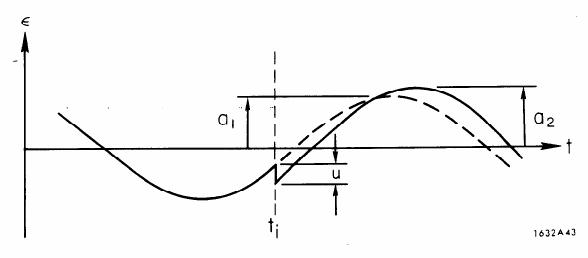
\includegraphics[width=0.8\linewidth]{./Figuras/fig43.jpeg}
	\caption{Effect on the energy oscillations of the emission of a quantum of energy $u$.}
	\label{fig:fig43}
\end{figure}
where\footnote{Obtained from $A^2 = \epsilon \epsilon^*$.}
\begin{align}
	A_1^2 = A_0^2 + u^2 - 2 A_0 u \cos \Omega (t_i - t_0),
\end{align}
and $t_1$ is some time displacement of no concern to us now. The quantum emission changes the amplitude of the oscillation to a new value which depends on the initial amplitude and on ($t_i - t_0$). Since the time $t_i$ at which a quantum emission occurs is completely unpredictable -- and since we are interested only in the cumulative affect of many such events -- we should ask only statistical questions. Such as: What is the probable amplitude change? In general, the phase ($t_i - t_0$) is completely random and the expectation value of $\cos\Omega(t_i - t_0)$ is therefore zero. Then, the probable amplitude change due to the quantum event is
\begin{align}\label{eq:5.25}
	\mean{\delta A^2} = \mean{A_1^2 - A_0^2} = \mean{u^2}
\end{align}
Notice that our result says that the probable change in $A^2$, which occurs when we add with random phase a new increment of oscillation of amplitude $u$, is just $u^2$ -- the same result we would have obtained for $\delta A^2$ if we had started with $A = 0$.\\
Suppose now that such quantum events occur in a random time sequence at the mean rate $\mathscr{N}$ (number per unit time). Each event changes $A^2$ by $u^2$; and since the mean time between events is $1/\mathscr{N}$, we expect that
\begin{align}\label{eq:5.26}
	\mean{\dfrac{dA^2}{dt}} = \mathscr{N} \mean{u^2}.
\end{align}
But the probable rate-of-change of $A^2$ is equal to the rate-of-change of the probable value of $A^2$ or
\begin{align} \label{eq:5.27}
	\dfrac{d}{dt}\mean{A^2} = \mathscr{N} \mean{u^2}.
\end{align}
In addition to exciting energy oscillations, the quantized energy losses contribute to a cumulative energy change. We have however, considered such average effects earlier. Their effect is to produce the energy oscillations as well as to cause the slow exponential damping of the amplitude $A$ with a time constant $\tau_\epsilon= 1/\alpha_\epsilon$. With such damping the amplitude decreases at the rate $A/\tau_\epsilon$; or its square at the rate $2A^2/\tau_\epsilon$. The probable amplitude must be similarly decreased by the damping which would contribute to the rate-of-change of $\mean{A^2}$ the amount
\begin{align} \label{eq:5.28}
	\dfrac{d}{dt}\mean{A^2} = -2 \dfrac{\mean{A^2}}{\tau_\epsilon}.
\end{align}
When both quantum excitation and damping are at work -- and other conditions are
stationary -- the rates of Eqs. \eqref{eq:5.27} and \eqref{eq:5.28} must sum to zero. We find that the probable value of $A^2$ is given by
\begin{align}
	\mean{A^2} = \dfrac{1}{2} \tau_\epsilon \mathscr{N} \mean{u^2}.
\end{align}
For the sinusoidal energy oscillations (as they are very nearly) the expectation value of $\epsilon$ is zero, and of its square -- which we shall call $\sigma_\epsilon^2$ -- is just $1/2$ the probable amplitude squared:
\begin{align}\label{eq:5.30}
	\sigma_\epsilon^2 = \mean{\epsilon^2} = \dfrac{\mean{A^2}}{2} = \dfrac{1}{4} \tau_\epsilon \mathscr{N} \mean{u^2}.
\end{align}
This then, would be the mean-square energy fluctuation in the energy oscillation which would be produced by the random emission of quanta.\\
An approximately equivalent result can be obtained from the following simple argument: The typical energy fluctuation comes from the deviation from its mean of the number of quanta emitted in one damping time $\tau_\epsilon$. The mean number emitted in $\tau_\epsilon$ is $\mathscr{N}\tau_\epsilon$, and so the rms deviation from the mean is $\sqrt{\mathscr{N}\tau_\epsilon}$ (Poisson distribution). Since each quantum has about the energy $u_c$, on the average,
\begin{align}
	\sigma_\epsilon = \sqrt{\mathscr{N}\tau_\epsilon} u_c.
\end{align}
The result is roughly the same as Eq.~\eqref{eq:5.30}. It is amusing to notice that, since $\mathscr{N} \approx P_\gamma/u_c$ and $\tau_\epsilon \approx E_0/P_\gamma$, we may also write that
\begin{align} \label{eq:5.32}
	\sigma_\epsilon \approx \sqrt{E_0 u_c}.
\end{align}
The energy fluctuation is roughly the geometric mean between the electron energy and the critical
 photon energy!\\
Let's now do a precise calculation which is somewhat more complicated -- first, because there is a distribution of quantum sizes and second, because both the distribution and the mean rate may vary around the storage ring. Returning to Eq.~\eqref{eq:5.28} we should consider separately the contribution to $d\mean{A^2}/dt$ from each interval of quantum sizes. Those quanta with energies between $u$ and $u + \Delta u$ -- of which there are $n(u)\Delta u$ - will give the contribution
\begin{align}
	\Delta \left\lbrace \dfrac{d}{dt}\mean{A^2} \right\rbrace = u^2 n(u) \Delta u.
\end{align}
But since the emission of quanta at the various different energies is also uncorrelated, each energy will contribute independently to the random-walk growth of $\mean{A^2}$. We need only sum the contributions from each interval $\Delta u$:
\begin{align}
	\dfrac{d}{dt}\mean{A^2} = \int_0^\infty u^2 n(u) du.
\end{align}
You will recognize the integral as just the product $\mathscr{N}\mean{u^2}$ considered in the preceding section -- Eq.~\eqref{eq:5.17}:
\begin{align}
	\dfrac{d}{dt} \mean{A^2} = \mathscr{N} \mean{u^2}.
\end{align}
The rate of growth just obtained depends on the electron energy -- which we may take to be the nominal energy $E_0$ -- and on $\rho$, the local radius of curvature of the trajectory, both of which may vary around the ring. From our derivation we may expect that the time for a ``significant'' change in the amplitude of the energy oscillation will be of the order of the damping time constant $\tau_\epsilon$. Since both the period of the oscillation $\approx 1/\Omega$,
 and the damping time $\tau_\epsilon$ are each much longer than a revolution time $T_0$ we may, without injustice, replace the rapidly varying quantity $\mathscr{N}\mean{u^2}$ by its mean value over one revolution of the ring. We shall also make a negligible error (on the average) if we replace the instantaneous radius of curvature $\rho$ of the trajectory at each azimuth $s$ by the local radius of curvature of the design orbit. Taking the average of $\mathscr{N}\mean{u^2}$
 over one revolution by integrating with respect to the azimuthal coordinate $s$, we may define\footnote{The index s on the brackets indicates that the average is taken over the coordinate $s$ as distinct from the average of $u^2$ which is over the distribution in $u$.},
\begin{align}
	Q_\epsilon = \mathscr{N}\mean{\mean{u^2}}_s = \dfrac{1}{L} \oint \mathscr{N} \mean{u^2} ds.
\end{align}
Following through the rest of the derivation as before we get for the mean-square energy fluctuation:
\begin{align} \label{eq:5.37}
	\sigma_\epsilon^2 = \dfrac{1}{4} \tau_\epsilon Q_\epsilon.
\end{align}
The simple form of our result is misleading; the complexities are hidden in $\tau_\epsilon$ and $Q_\epsilon$. Let's look first at $Q_\epsilon$. We need to evaluate $\mathscr{N} \mean{u^2}$ on the design orbit.\\
Suppose we begin with the form derived in Eq.~\eqref{eq:5.18}. $P_\gamma$ on the design orbit is
obtained from Eq.~\eqref{eq:4.4} by setting $E = E_0$ and $(1/\rho) = G$ (see Section~\ref{sec:2.2}), so
\begin{align}
	(P_\gamma)_\text{design orbit} = \dfrac{c C_\gamma}{2\pi} E_0^4 G^2,
\end{align}
which may be written -- using Eq.~\eqref{eq:4.9} -- as
\begin{align}
	(P_\gamma)_\text{design orbit} = \dfrac{\mean{P_\gamma}_s G^2}{\mean{G^2}_s}.
\end{align}
And $u_c$ on the design orbit is from Eq.~\eqref{eq:5.9},
\begin{align} \label{eq:5.40}
	(u_c)_\text{design orbit} = \dfrac{3}{2} \hslash c \gamma_0^3 |G|.
\end{align}
Then, we have that
\begin{align} \label{eq:5.41}
	\left( \mathscr{N} \mean{u^2} \right)_\text{design orbit} = C_u \dfrac{3}{2} \hslash c \gamma_0^3 |G| \dfrac{\mean{P_\gamma}_s G^2}{\mean{G^2}_s}
\end{align}
The only quantity which varies around the design orbit is $G$ so that $Q_\epsilon$, can be written as\footnote{We may now leave off the subscripts on the average since it is clear that all
quantities shown are to be averaged over $s$. I hope it is clear that $\mean{G^2}$, for example, means $\oint G^2(s)ds/L$ where $L$ is the orbit length.}
\begin{align}
	Q_\epsilon = \dfrac{3}{2} C_u \hslash c \gamma_0^3 P_\gamma \dfrac{\mean{|G|^3}}{\mean{G^2}}.
\end{align}
Taking $\tau_\epsilon$ from Eq.~\eqref{eq:4.53},
\begin{align}
	\tau_\epsilon = \dfrac{2E_0}{J_\epsilon \mean{P_\gamma}},
\end{align}
we may finally rewrite Eq.~\eqref{eq:5.37} as
\begin{align}
	\sigma_\epsilon^2 = \dfrac{3 C_u \hslash mc^3 \gamma_0^4 \mean{|G|^3}}{4 J_\epsilon \mean{G^2}}.
\end{align}
The relative energy spread $\sigma_\epsilon/E_0$ is usually more significant. We may write it as
\begin{align}\label{eq:5.45}
	\left(\dfrac{\sigma_\epsilon}{E_0}\right)^2 = \dfrac{C_q \gamma_0^2}{J_\epsilon} \dfrac{\mean{|G|^3}}{\mean{G^2}},
\end{align}
with $C_q$ -- which we may call the quantum constant -- given by
\begin{align} \label{eq:5.46}
	C_q = \dfrac{3 C_u \hslash}{4mc} = \dfrac{55}{32\sqrt{3}} \dfrac{\hslash}{mc} = 3.84 \times 10^{-13}\,\text{meter}.
\end{align}
It is very nearly, just the Compton wavelength of the electron.\\
The quantity $\mean{|G|^3}/J_\epsilon \mean{G^2}$ is a geometrical property of the guide field. Specifically,
\begin{align}
	\dfrac{\mean{|G|^3}}{J_\epsilon \mean{G^2}} = \dfrac{1}{J_\epsilon} \dfrac{\oint |G^3(s)|ds}{\oint G^2(s) ds}.
\end{align}
It is roughly equal to the inverse of the ``typical'' radius-of-curvature of the design orbit. The result of Eq.~\eqref{eq:5.45} is then roughly $\gamma^2$ times the ratio of the Compton wavelength to the orbit radius. For any ring the quantum induced spread in the relative energy deviation - namely $\sigma_\epsilon/E_0$ varies in direct proportion to the electron energy.\\
In a storage ring with an isomagnetic guide field (one which has a constant radius $\rho_0$ in the magnets and is straight elsewhere) the geometrical expression above is just $1/J_\epsilon \rho_0$, and
\begin{align}\label{eq:5.48}
	\left( \dfrac{\sigma_\epsilon}{E_0}\right)^2 = \dfrac{C_q \gamma_0^2}{J_\epsilon \rho_0}, && \text{(isomag.)}
\end{align}
In an isomagnetic storage ring with a 5 meter magnetic radius, electrons stored with an energy of 1 GeV will have an energy spread very nearly 0.04\% of the energy -- or about 40 keV.

    \section{Distribution of the Fluctuations}\label{sec:5.3}

The energy deviation $\epsilon$ at any instant $t$ is the result of a superposition of the
contributions from the emission of quanta at all earlier times $t_i$. We may in fact, write for $\epsilon(t)$
\begin{align} \label{eq:5.49}
	\epsilon(t) = \sum_{t_i<t} u_i e^{-(t-t_i)\tau_\epsilon}\cos\Omega(t-t_i),
\end{align}
where $u_i$ is the energy of the quantum emitted at $t_i$. Since the typical value of $\epsilon(t)$ is much larger than the typical quantum energy -- see Eq.~\eqref{eq:5.32} -- and since the times $t_i$ are randomly distributed, the sum at any instant $t$ consists of contributions from a large number of small terms which are all statistically independent, and which are positive and negative with equal probability. It is well known\footnote{And follows from the Central Limit Theorem of probability theory.} that the result of such a sum is a stochastic quantity whose most probable value is zero and which is otherwise distributed as a normal error function -- a so-called Gaussian distribution. That is the probability $w(\epsilon)d\epsilon$ that the energy deviation
will be found in an interval $d\epsilon$ at $\epsilon$ is distributed according to
\begin{align}\label{eq:5.50}
	w(\epsilon)d\epsilon = \dfrac{1}{\sqrt{2\pi}\sigma_\epsilon} \exp{(-\epsilon^2/\sigma_\epsilon^2)}d\epsilon.
\end{align}
The parameter $\sigma_\epsilon$, often called the standard deviation, is equal to the root-mean-
Square spread of the distribution -- that is, the square root of $\mean{\epsilon^2}$ -- as can
easily be shown by a direct integration:
\begin{align}
	\sigma_\epsilon^2 = \int_{-\infty}^{\infty} \epsilon^2 w(\epsilon) d\epsilon.
\end{align}
(The distribution function $w(\epsilon)$ is properly normalized so that its complete integral
is equal to 1) The standard deviation $\sigma_\epsilon$ is then, the same quantity we have evaluated in the preceding section.\\
In a stored beam we have, normally, a large number $N$ of stored electrons. So long as any interactions among them can be ignored, the distribution of energies within the bunch will -- under stationary conditions -- also be described by Eq.~\eqref{eq:5.50}. That is, the number of electrons with energies between $\epsilon$ and $\epsilon+d\epsilon$ will be just $Nw(\epsilon)d\epsilon$. And the ``half-width'' of the spread of energies in the beam is described by $\sigma_\epsilon$.\\
The distribution function of Eq.~\eqref{eq:5.50} and also our calculation of $\sigma_\epsilon$ assume that the energy oscillations are linear (with nonlinearities, Eq.~\eqref{eq:5.49} is not
correct and the effects of the individual quanta are no longer independent). We have already seen however, that the energy oscillations are not linear for large energy deviations. If the rf voltage function is significantly nonlinear over the time displacements that correspond to the likely energy deviations, we must expect the probability distribution for $\epsilon$ to be distorted from the ideal distribution of Eq.~\eqref{eq:5.50}. If, however, the nonlinearity
 is not too great over the largest part of the distribution, we may expect that neither $\sigma_\epsilon$; nor the distribution function of the energy deviations will be affected very much.\\
The distribution of energy deviations just considered implies related distributions in other parameters of the energy oscillations. The relationships are most easily understood by considering the electron's trajectory in a ``phase diagram'' such as the one discussed in Section~\ref{sec:3.5}. Suppose we describe the state of the energy oscillation by giving its energy deviation $\epsilon$ and its ``scaled'' time displacement $\theta$, which we define by
\begin{align} \label{eq:5.52}
	\theta = \dfrac{\Omega E_0}{\alpha} \tau.
\end{align}
$\Omega$, the angular frequency of the energy oscillation and $\alpha$, the dilation factor are
constants so $\theta$ is just a scaled equivalent of $\tau$ the time displacement coordinate of
the energy oscillations (See Section~\ref{sec:3.5}). So long as the damping rate is small, $\theta$ could equally well be defined by
\begin{align}
	\theta = \dfrac{1}{\Omega} \dfrac{d\epsilon}{dt},
\end{align}
so it may also be viewed as a normalized derivative of $\epsilon$. We may now represent the state of motion of an electron by a point on a two-dimensional graph in which $\epsilon$ and $\theta$ are orthogonal coordinates -- see Fig.~\ref{fig:fig44}(a) -- and in which an oscillation
of constant amplitude would describe a circle. Then so long as the damping and the quantum effects are small, we may consider that for any small interval of time, $\epsilon$ and $\theta$ vary as
\begin{align}
	\epsilon &= A \cos\varphi,\\
    \theta &= A \sin\varphi;
\end{align}
where
\begin{align}
	\varphi = \Omega t - \varphi_0,
\end{align}
and $A$ is slowly varying amplitude. The quantities $A$ and $\varphi$ are a polar representation of the representative point and $\varphi$ increases as $\Omega t$.
\begin{figure}[!htb]
	\centering
	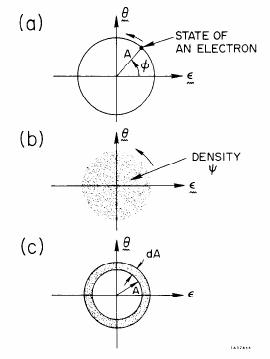
\includegraphics[width=0.8\linewidth]{./Figuras/fig44.jpeg}
	\caption{Scaled phase space of the energy oscillations.}
	\label{fig:fig44}
\end{figure}
The distribution of energy oscillations of the electrons in a stored bunch can now be represented
 by a distribution of points in the phase plot as indicated schematically in Fig.~\ref{fig:fig44}b. A complete description of the distribution is given by specifying the density $\Psi(\epsilon,\theta)$ in the $\epsilon,\theta$ plane. That is $\Psi(\epsilon,\theta) d\epsilon d\theta$ is to represent the number of electrons found in the element of area $d\epsilon d\theta$ located at $(\epsilon,\theta)$. We already know the projection of $\Psi(\epsilon,\theta)$ on the horizontal axis. If there are $N$ electrons in the bunch it is just $N w(\epsilon)$. But in one-quarter of an oscillation each electron rotates one-quarter of a revolution about the origin of the figure. And since we are assuming a stationary distribution
 -- that is one with no time variations -- the projection on the vertical and on the horizontal
 axes must be identical. It must be then, that the number of electrons in an element of area $d\epsilon d\theta$ is given by
\begin{align} \label{eq:5.57}
	\Psi(\epsilon,\theta)d\epsilon d\theta = \dfrac{N}{2\pi \sigma_\epsilon^2} \exp\left( -\dfrac{\epsilon^2 + \theta^2}{2\sigma_\epsilon^2} \right) d\epsilon d\theta.
\end{align}
The projection on the horizontal axis is
\begin{align}
	\int_{-\infty}^{\infty} \Psi(\epsilon,\theta) d\theta = \dfrac{N}{\sqrt{2\pi} \sigma\epsilon} \exp\left( -\dfrac{\epsilon^2}{2\sigma_\epsilon^2} \right) d\epsilon,
\end{align}
which agrees with the $w(\epsilon)$ of Eq.~\eqref{eq:5.50}. Similarly, the distribution in $\theta$ is
\begin{align}
	\dfrac{N}{\sqrt{2\pi} \sigma_\epsilon} \exp\left( -\dfrac{\theta^2}{2\sigma_\epsilon^2} \right) d\theta.
\end{align}
We may now ask what is the distribution of oscillations amplitudes. Since $A^2 = \epsilon^2 + \theta^2$, the density of electrons in the $\epsilon,\theta$ plane at the amplitude $A$ is just
\begin{align}
	\dfrac{N}{2\pi \sigma_\epsilon^2} \exp\left( -\dfrac{A^2}{2\sigma_\epsilon^2} \right).
\end{align}
If we now let $g(A)dA$ be the number of electrons in an amplitude interval $dA$ at $A$, that number is just $2\pi A dA$ times the density at A:
\begin{align}
	g(A) dA = \dfrac{N A}{\sigma_\epsilon^2} \exp\left( -\dfrac{A^2}{2\sigma_\epsilon^2} \right) dA.
\end{align}
(See Fig.~\ref{fig:fig44}(c)) The mean-square of $A$ in this distribution is just the $\mean{A^2}$ that was discussed in the preceding section. By direct integration of $A^2 g(A) dA$ you can see that $\mean{A^2} = 2\sigma_\epsilon^2$, as was argued earlier. So the last equation can be written as
\begin{align}
	g(A) dA = N \dfrac{2 A}{\mean{A^2}} \exp\left( -\dfrac{A^2}{\mean{A^2}} \right) dA.
\end{align}
Suppose we take the number $W = A^2$ as a measure of the ``oscillation energy''\footnote{W is proportional to -- but different by a numerical factor from -- the ``oscillation energy'' defined in Section~\ref{sec:3.6}.}, and compute the mean oscillation energy $\mean{W}$. Since the energy interval $dW$ corresponds to $2AdA$, the number of electrons which are found in the interval
 $dW$ at $W$ is
\begin{align} \label{eq:5.62}
	h(W)dW = \dfrac{N}{\mean{W}}\exp\left( -\dfrac{W}{\mean{W}} \right) dW.
\end{align}
The distribution
 in oscillation energies is a pure exponential and corresponds to the Boltzman distribution of energies in an ensemble of mechanical systems in thermal equilibrium -- with the characteristic
 energy $\mean{W}$ given by
\begin{align}
	\mean{W} = \mean{A^2} = 2 \sigma_\epsilon^2.
\end{align}

    \section{Bunch Length}\label{sec:5.4}

We have just seen that the distribution in the normalized time displacement $\theta$ is as a Gaussian with a standard deviation that is equal to the standard deviation $\sigma_\epsilon$ of the energy oscillations -- refer to Eq.~\eqref{eq:5.50}. It follows that the fluctuating energy oscillations are accompanied by associated fluctuations in the time displacement $\tau$, and that the standard deviation $\sigma_\tau$ of these fluctuations is -- see Eq.~\eqref{eq:5.52} --
\begin{align}
	\sigma_\tau = \dfrac{\alpha}{\Omega E_0} \sigma_\epsilon.
\end{align}
For an isomagnetic guide field Eq.~\eqref{eq:5.45} gives
\begin{align}
	\sigma_\tau^2 = \dfrac{\alpha^2}{\Omega^2} \dfrac{C_q \gamma_0^2}{J_\epsilon \rho_0} && \text{(isomag).}
\end{align}
Taking $\Omega^2$ from Eq.~\eqref{eq:3.44}
\begin{align}
	\sigma_\tau^2 = \dfrac{\alpha T_0 E_0}{e\dot{V}_0} \dfrac{C_q \gamma_0^2}{J_\epsilon \rho_0} = \dfrac{C_q}{(mc^2)^2} \dfrac{\alpha L}{J_\epsilon \rho_0 c} \dfrac{E_0^3}{e \dot{V}_0} && \text{(isomag).}
\end{align}
The spread $\sigma_\tau$ in the time displacement gives when multiplied by $c$, also the spread
of longitudinal displacement from the bunch center -- or, what we may call the bunch half-length.\\
If the energy $E_0$ of the stored beam in a particular storage ring is varied while holding constant the slope of the rf voltage ($\dot{V}_0$), the bunch length will increase with the energy as $E_0^{3/2}$.\\
In several of the storage rings that have been constructed to date the bunch length is observed to be larger than is predicted here by a significant factor which depends on the number of electrons
 in the stored bunch.

    \section{Beam Width} \label{sec:5.5}

The emission of discrete quanta in the synchrotron radiation will also excite random betatron oscillations and these quantum-induced oscillations are responsible for the lateral extent of a stored electron beam. Let's look first at the quantum effects on the horizontal betatron oscillations (as in the preceding section, I will consider first only the gross statistical
 properties of the fluctuations).\\
In Section~\ref{sec:4.3} we considered the effect of a small radiation loss $\delta E$ -- which
was assumed there to occur continuously in a path length $\delta \ell$ -- under the assumption that the momentum loss was parallel to the direction of motion. We may take over the results obtained there and adapt them to the case of quantum emission by setting $\delta E$ to the quantum
 energy $u$ -- keeping for the moment the assumption that quantum emission gives only a change in the magnitude of the momentum and not in its direction. You will recall from Section~\ref{sec:4.3} that a change in energy is accompanied by a change in the betatron displacement only because of the sudden displacement of the reference orbit -- the energy displaced orbit -- about which
the betatron oscillations occur. Taking the results of Eqs. \eqref{eq:4.35} and \eqref{eq:4.38},
 the emission of a quantum of energy $u$ will result in a change $\delta x_\beta$ in the betatron displacement and a change $\delta x_\beta'$ in the betatron slope given by
\begin{align}\label{eq:5.67}
	\delta x_\beta = -\eta \dfrac{u}{E_0}; && \delta x_\beta' = -\eta' \dfrac{u}{E_0}.
\end{align}
The effect that such a sudden disturbance will have on the betatron oscillations will depend on where in the storage ring the quantum emission occurs -- and on where we observe the oscillation.
 From Section~\ref{sec:2.6} we know how to relate the oscillations observed at one azimuth to those that will be found at another azimuth; so we can for convenience, evaluate the quantum effects by what they do to the oscillations at some fixed azimuth -- say at $s_1$ -- and later transfer the result to any other azimuth. Our program can then be the following: (1) We ask what is
the effect at $s_1$ of a quantum emission that occurs at some other azimuth $s_2$. (2) We average over all quanta which might be emitted at $s_2$. (3) We sum the contributions from all possible values of $s_2$.\\
In Section~\ref{sec:2.6} we considered the motion which resulted at $s_1$ from the ``initial
conditions'' $x_2$ and $x_2'$ at $s_2$, the result can be written in the form\footnote{It will be understood that here $\beta$ means $\beta_x$}
\begin{align} \label{eq:5.68}
	x_\beta(s_1,t_j) = a \sqrt{\beta_1} \cos \varphi_j,
\end{align}
where the $\varphi_j$ are the oscillation phases at the times $t_j$ of the successive passages
of the electron by the azimuth $s_1$, $\beta_1$ is the betatron function at $s_1$ and $a$ is an
invariant amplitude factor given by
\begin{align}
	a^2 = \dfrac{1}{\beta_2} \left\lbrace x_2^2 + \left( \beta_2 x_2' - \dfrac{\beta_2'}{2} x_2 \right)^2 \right\rbrace.
\end{align}
If we put for $x_2$ and $x_2'$ the disturbance of Eq.~\eqref{eq:5.67} and write $\delta a^2$ for the resulting amplitude, we have that the emission of a quantum of energy $u$ at $s_2$ gives the
mean amplitude change (in respect to phase)
\begin{align} \label{eq:5.70}
	\mean{\delta a^2} = \dfrac{u^2}{E_0^2} \dfrac{1}{\beta_2} \left\lbrace \eta_2^2 + \left( \beta_2 \eta_2' - \dfrac{\beta_2'}{2} \eta_2 \right)^2 \right\rbrace.
\end{align}
To obtain this result, it is necessary to use the following relations
\begin{align*}
	\delta(x^2) = 2 x \delta x + (\delta x)^2 & \Rightarrow \mean{\delta x^2} = \mean{\delta x}^2,\\
    \delta(x'^2) = 2 x' \delta x' + (\delta x')^2 & \Rightarrow \mean{\delta x'^2} = \mean{\delta x'}^2,\\
    \delta(x x') = x \delta x' + x' \delta x + \delta x \delta x' & \Rightarrow \mean{\delta (x x')} = \mean{\delta x} \mean{\delta x'}.
\end{align*}
All of the $s$-dependent quantities on the right-hand-side are to be evaluated at $s_2$, so let's define a new function of $s$:
\begin{align} \label{eq:5.71}
	\mathscr{H}(s) = \dfrac{1}{\beta} \left\lbrace \eta^2 + \left( \beta \eta' - \dfrac{\beta'}{2} \eta \right)^2 \right\rbrace.
\end{align}
which is specified by the properties of the guide field. Then Eq.~\eqref{eq:5.70} becomes
simply
\begin{align} \label{eq:5.73}
	\mean{\delta a^2} = \dfrac{u^2}{E_0^2} \mathscr{H}(s_2).
\end{align}
We now know what will be the result if a quantum is emitted at $s_2$; we must next ask what is the likelihood that such an event will occur. Consider what happens as the electron travels the distance $\Delta s$ at $s_2$ -- which will take the time $\Delta t = \Delta s/c$. Taking the definitions of Section~\ref{sec:5.1}, the expected number of quantum events is $\mathscr{N}\Delta s/c$, and the probable value of $u^2$ for the quantum emitted is $\mean{u^2}$. So the change in the probable value of $a^2$ due to the element $\Delta s$ of the trajectory
 can be written as
\begin{align} \label{eq:5.74}
	\mean{\delta a^2} = \dfrac{\left\lbrace \mathscr{N} \Delta s \mean{u^2} \mathscr{H}(s) \right\rbrace_2}{c E_0^2}.
\end{align}
The subscript on the curly brackets means that all quantities inside are to be evaluated at $s_2$ (both $\mathscr{N}$ and $\mean{u^2}$, you will remember, depend on the local radius-of-curvature of the trajectory).\\
Suppose we now add up the contributions to changes in $\mean{a^2}$ during one trip of the electron around the ring. The resulting change, which we may call $\Delta \mean{a^2}$, is obtained by integrating the right-hand-side of Eq.~\eqref{eq:5.74} once around the ring:
\begin{align}
	\Delta \mean{a^2} = \dfrac{1}{c E_0^2} \oint \left\lbrace \mathscr{N} \mean{u^2} \mathscr{H}(s) \right\rbrace_2 ds_2.
\end{align}
As before\footnote{For the remainder of the development I shall follow the same line of argument used in the preceding section and will not repeat all of the details. You should refer to
that section for any details that are not clear.}, it will be convenient to represent the integral as the product of the length of the orbit $L$, with the mean value -- with respect to $s$ -- of the integrand.
\begin{align}\label{eq:5.76}
	\Delta \mean{a^2} = \dfrac{L}{c E_0^2} \mean{\mathscr{N}\mean{u^2}\mathscr{H}}_s.
\end{align}
Although $\mathscr{N}$ and $\mean{u^2}$ depend on the actual electron trajectory -- and so may change from one turn to the next -- they will differ little from the values on the design orbit.
 Also the differences will, to first order in the displacements from the design orbit, average to zero. Since we are going to be interested, anyway, only in effects which accumulate over many revolutions, we will make no significant error if we take (as we did for the energy oscillations)
 the average in Eq.~\eqref{eq:5.76} by evaluating $\mathscr{N}\mean{u^2}$ on the design orbit. We shall therefore, interpret the average over $s$ in that way.
The change $\Delta \mean{a^2}$ of Eq.~\eqref{eq:5.76} occurs in the time of one revolution, namely $L/c$. So we may write that
\begin{align} \label{eq:5.77}
	\dfrac{d}{dt} \mean{a^2} = Q_x \bydef \dfrac{\mean{\mathscr{N}\mean{u^2}\mathscr{H}}_s}{E_0^2}.
\end{align}
This is of course, only the contribution from the quantum noise. As in Section~\ref{sec:5.2}, we must still add in the average effect of the radiation which contributes a damping term
\begin{align} \label{eq:5.78}
	\dfrac{d}{dt} \mean{a^2} = - \dfrac{2 \mean{a^2}}{\tau_x},
\end{align}
where $\tau_x$ is the damping time constant of the radial betatron oscillations. Under stationary
 conditions the total time derivative -- the sum of Eqs. \eqref{eq:5.77} and \eqref{eq:5.78} is zero. We get for the stationary expectation value of $a^2$:
\begin{align}
	\mean{a^2} = \dfrac{1}{2} \tau_x Q_x.
\end{align}
We may now return to Eq. \eqref{eq:5.68} to get the expected spread in the betatron displacements. Squaring and taking the expectation of $x_\beta(s_1)$ we may write for the rms spread in the radial betatron displacement at $s_1$:
\begin{align} \label{eq:5.81}
	\sigma_{x_\beta}^2(s_1) = \mean{x_\beta^2(s_1)} = \dfrac{1}{2}\mean{a^2}\beta_1.
\end{align}
Since the azimuth $s_1$ may be anywhere, we may now drop the subscript. Combining the last two equations, we may write that
\begin{align}
	\sigma_{x_\beta}^2(s) = \dfrac{1}{4} \tau_x Q_x \beta(s).
\end{align}
The form of the result is similar to that obtained for $\sigma_\epsilon$. Both $\tau_x$ and $Q_x$, are numbers which are determined from the overall properties of the guide field -- and do not, therefore, vary with $s$. The only variation of $\sigma_{x_\beta}$ comes from the factor $\beta(s)$. This then is our result for the horizontal spread of a stored electron beam due to quantum induced betatron oscillations.\\
To see the physical significance of our result we must recover the complexities hidden in $\tau_x$ and $Q_x$. Taking $\mathscr{N}\mean{u^2}$ from Eq.~\eqref{eq:5.41}
\begin{align}
	Q_x = \dfrac{3}{2} C_u \hslash c \gamma_0^3 \dfrac{\mean{P_\gamma}_s \mean{|G|^3\mathscr{H}}_s}{\mean{G^2}},
\end{align}
where $G(s)$ is the inverse radius of the orbit, and, $\mathscr{H}(s)$ is the function of Eq.~\eqref{eq:5.71}. Taking $\tau_x$ from Eq.~\eqref{eq:4.53} we get that
\begin{align}
	\dfrac{\sigma_{x_\beta}^2}{\beta} = \dfrac{1}{4} \tau_x Q_x = \dfrac{C_q \gamma_0^2 \mean{|G|^3\mathscr{H}}_s}{J_x \mean{G^2}_s},
\end{align}
where $C_q$ is the quantum coefficient defined in Eq.~\eqref{eq:5.46}.\\
For an isomagnetic guide field ($G = 1/\rho_0$, or zero) the result simplifies to
\begin{align}\label{eq:5.84}
	\dfrac{\sigma_{x_\beta}^2}{\beta} =\dfrac{C_q \gamma_0^2 \mean{\mathscr{H}}_\text{Mag}}{J_x \rho_0} && \text{(isomag.),}
\end{align}
where $\mean{\mathscr{H}}_\text{Mag}$ is the average of $\mathscr{H}$ taken only in the magnets.
 That is,
\begin{align}\label{eq:5.85}
	\mean{\mathscr{H}}_\text{Mag} = \dfrac{1}{2\pi\rho_0} \int_\text{Mag} \dfrac{1}{\beta}\left\lbrace \eta^2 \left( \beta\eta' - \dfrac{\beta'}{2} \eta \right)^2 \right\rbrace ds.
\end{align}
Comparing Eq.~\eqref{eq:5.84} with Eq.~\eqref{eq:5.48} we see that for an isomagnetic guide
field we may write that
\begin{align}\label{eq:5.86}
	\dfrac{\sigma_{x_\beta}^2(s)}{\beta(s)} =  \dfrac{J_\epsilon \mean{\mathscr{H}}_\text{Mag}}{J_x} \left( \dfrac{\sigma_\epsilon}{E_0} \right)^2 && \text{(isomag.)}
\end{align}
For a precise calculation of $\sigma_{x_\beta}$ the integral of Eq.~\eqref{eq:5.85} must be evaluated.\\
As argued in Section~\ref{sec:5.3} for the energy deviations, the likelihood of finding
any particular betatron displacement will vary as a normal error function. That is, the probability of finding a particular electron with a betatron displacement between $x_\beta$ and $x_\beta + dx_\beta$ will be
\begin{align}
	w(x_\beta)dx_\beta = \dfrac{1}{\sqrt{2\pi} \sigma_{x_\beta}} \exp\left( -x_\beta^2/2\sigma_{x_\beta}^2 \right).
\end{align}
If we think of a particular bunch of electrons which contains, say, $N$ electrons, then as it passes any particular azimuth $s$, the number of electrons $n(x_\beta)$ which lie in the radial interval $dx_\beta$ at $x_\beta$ is
\begin{align*}
	n(x_\beta)dx_\beta = Nw(x_\beta)dx_\beta,
\end{align*}
and so has also a Gaussian distribution. We may think then, of a stored beam as a fuzzy object with a half-width (which depends on $s$) given by the standard deviation $\sigma_{x_\beta}$ of its distribution in radius.\\
We should not forget, however, that the total radial spread has contributions from both the betatron and energy oscillations, since the spread of energies of the electrons in a bunch gives rise to an associated radial spread. Recalling that an electron with the energy deviation $\epsilon$ moves on an orbit whose radial displacement varies with the azimuthal position $s$ according to $x_\epsilon(s) = \eta(s) \epsilon/E_0$, it follows that the mean-square radial spread due to the energy spread is
\begin{align}
	\sigma_{x_\epsilon}^2(s) = \eta^2(s) \dfrac{\sigma_\epsilon^2}{E_0^2}.
\end{align}
Now the periods of the energy oscillations and of the betatron oscillations are widely different, and certainly not precisely commensurate. We may, therefore, consider that -- although they are stimulated by the same stochastic events -- they will be statistically independent. We may then add their contribution to the total
radial spread as the squares and write that
\begin{align}
	\sigma_x^2 = \sigma_{x_\beta}^2 + \sigma_{x\epsilon}^2.
\end{align}
Let's consider only an isomagnetic guide field. Taking $\sigma_{x_\beta}^2$ from Eq.~\eqref{eq:5.86} and using Eq.~\eqref{eq:5.48} for $\sigma_\epsilon^2$, we may write that
\begin{align}
	\sigma_x^2(s) = \dfrac{C_q\gamma_0^2}{\rho_0} \left\lbrace \dfrac{\mean{\mathscr{H}}_\text{Mag} \beta(s)}{J_x} + \dfrac{\eta^2(s)}{J_\epsilon} \right\rbrace && \text{(isomag.)}.
\end{align}
The results of the section do not take into account the effects of coupling between radial and vertical oscillations. If such coupling exists the results must be modified as described in the following section.

    \section{Beam Height} \label{sec:5.6}

In calculating the beam width we assumed that the emission of a quantum did not change the direction of motion of the electron. This assumption is not strictly correct. Any individual
 quantum event may give a small transverse impulse to the electron. We may think that the quantum event corresponds to the emission of a photon of momentum $u/c$ at, say the angle $\theta_\gamma$ with respect to the electron's momentum. It will carry off a transverse component of momentum equal to $\theta_\gamma u/c$. Conservation of momentum requires that there be a corresponding
 change in the transverse momentum $x'E_0/c$ of the electron -- see Fig.~\ref{fig:fig45}. That is there will be a change in $x'$ given by
\begin{align} \label{eq:5.98}
	\delta x' = \dfrac{u}{E_0} \theta_{x},
\end{align}
\begin{figure}[!htb]
	\centering
	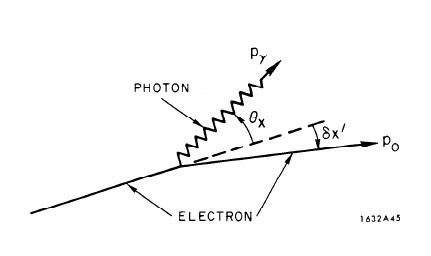
\includegraphics[width=0.8\linewidth]{./Figuras/fig45.jpeg}
	\caption{Change in the direction of an electron due to the emission of a photon.}
	\label{fig:fig45}
\end{figure}
where $\theta_x$ is the horizontal projection of $\theta_\gamma$. The synchrotron radiation
 is emitted generally along the direction of motion of the electron, but is spread out in a cone of half-angle $1/\gamma$. So we may consider that $\theta_\gamma$ is typically of the order of $1/\gamma$. The quantity $\eta'$ which appears in Eq.~\eqref{eq:5.67} is of order-of-magnitude
 1, so the neglect of the contribution from \eqref{eq:5.98} on the radial motion was well justified.\\
Consider however, what may be the quantum effects on the vertical betatron motion. If the design orbit lies strictly in a plane there are no first-order effects from quantum emission on the vertical motion (that is, the vertical function which corresponds to is precisely zero). The only remaining effect would be from the angular distribution of the radiation. Let's see what the magnitude of effect would be.\\
We may take over the results of the preceding section by replacing Eq.~\eqref{eq:5.67} by
\begin{align}
	\delta z = 0; && \delta z' = \dfrac{u}{E_0} \theta_z,
\end{align}
where $\theta_z$ is the projected vertical angle of emission of the photon. Equation~\eqref{eq:5.73} would become -- using the subscript $z$ to remind us that we are now dealing with a vertical oscillation --
\begin{align}
	\delta\mean{a_z^2} = \dfrac{u^2}{E_0^2} \theta_z^2 \beta_z (s_2).
\end{align}
Following through the derivations we would find in place of Eq.~\eqref{eq:5.81}
\begin{align}
	\sigma_{z\beta}^2(s) = \dfrac{1}{4} \tau_z Q_z \beta_z(s),
\end{align}
with,
\begin{align}
	Q_z = \dfrac{\mean{\mathscr{N}\mean{u^2 \theta_z^2}\beta_z}_s}{E_0^2}.
\end{align}
To evaluate $Q_z$ we would need to take into account the variation of the frequency spectrum of synchrotron radiation with the angle of emission. Since the effect we are dealing with is in any case small, an approximate calculation will do. Suppose we first make the approximation
\begin{align}
	\mean{u^2 \theta_z^2} \approx \mean{u^2}\mean{\theta_z^2}.
\end{align}
For the mean-square projected angle, we may take $1/2$ the mean-square polar angle of the radiation
\begin{align}
	\mean{\theta_z^2} \approx \dfrac{1}{\gamma_0^2}.
\end{align}
Also let's replace $\beta_z(s)$ by a typical value $\beta_n$. We then get that
\begin{align}
	Q_z \approx \dfrac{\mean{\mathscr{N}\mean{u^2}}_s\beta_n}{\gamma_0^2 E_0^2}.
\end{align}
Recall that the average of $\mathscr{N}\mean{u^2}$ is just what we called $Q$ in Section~\ref{sec:5.2}. We may then write that
\begin{align}
	\dfrac{\sigma_z^2}{\sigma_\epsilon^2} \approx \dfrac{\tau_z Q_z \beta_n}{\tau_\epsilon Q_\epsilon} \approx \dfrac{J_\epsilon}{J_z} \dfrac{\beta_n^2}{\gamma_0^2 E_0^2}.
\end{align}
For a flat design orbit $J_z \approx 1$. Considering only the isomagnetic case, we may take $\sigma_\epsilon^2/E_0^2$ from Eq.~\eqref{eq:5.48} and get
\begin{align} \label{eq:5.107}
	\sigma_z^2 \approx \dfrac{C_q \beta_n^2}{\rho_0} && \text{(isomag.)}
\end{align}
Roughly speaking, $\beta_n$ is the same order as $\rho_0$ and
\begin{align}
	\sigma_z^2 \approx C_q \beta_n.
\end{align}
The vertical oscillations induced by the quantum emission are energy independent and less than the radial oscillations by roughly the factor $1/\gamma_0^2$. They are very small indeed.\\
The vertical oscillations given by Eq.~\eqref{eq:5.107} are so small that they will always be negligible in comparison with the vertical oscillations produced by another much larger effect -- a coupling of oscillation energy from the horizontal betatron oscillations into the vertical
 ones. We did not analyze such effects when we were considering, in Part II, the nature of the betatron oscillations because they would be essentially perturbations of second order. An analysis of the perturbations expected from the construction imperfections in a real ring shows that the coupling between horizontal and vertical oscillations is likely to produce a beam height in the ring which is at least a few percent of the beam width -- and is therefore much larger than the minimum intrinsic width calculated above.\\
Indeed, it is -- as we shall see later -- sometimes desirable to obtain a beam height larger than is produced by accidental imperfections. And this can be done by introducing an intentional
 augmentation of the coupling between the horizontal and vertical oscillations -- as can be effected by special magnetic elements (skew quadrupoles) or by operating the ring near a resonance between $\nu_x$ and $\nu_z$, or by a combination of the two.\\
A detailed analysis of the coupling of vertical and horizontal oscillations is beyond the scope of this report, but a phenomenological approach will serve our purposes. Suppose we let $\varepsilon_x$ and $\varepsilon_z$ represent the invariant mean-square amplitudes of the radial and vertical oscillations. That is,
\begin{align} \label{eq:5.109}
	\varepsilon_x = \dfrac{\sigma_x^2(s)}{\beta_x(s)}; && \varepsilon_z = \dfrac{\sigma_z^2(s)}{\beta_z(s)}.
\end{align}
For the special case in which the damping rates of the vertical and horizontal oscillations are equal, we may now argue as follows. In the absence of coupling
\begin{align}
	\varepsilon_x = \varepsilon_0 = \dfrac{1}{4} \tau_x Q_x.
\end{align}
-- from Eq.~\eqref{eq:5.81}. When coupling is taken into account, the quantum excitation of the radial oscillations can be shared with the vertical oscillations in any proportion up to an equal division. That is, we may have that
\begin{align}
	\varepsilon_z = \varkappa \varepsilon_x,
\end{align}
where $\varkappa$ is the ``coefficient of coupling''. In principle $\varkappa$ may be any number between
0 and 1, although it is probably difficult in practice to reduce $\varkappa$ below one percent or so. Since the excitation is being shared, the combined excitations must still be equal to $\varepsilon_0$.
\begin{align}
	\varepsilon_x + \varepsilon_z = \varepsilon_0.
\end{align}
We may equivalently write that
\begin{align}
	\varepsilon_z &= \dfrac{\varkappa}{1+\varkappa}\varepsilon_0,\\
    \varepsilon_x &= \dfrac{1}{1+\varkappa}\varepsilon_0.
\end{align}
The excitation $\varepsilon_0$ is to be taken from any of the expressions for $\sigma_{x\beta}^2/\beta$ derived (without taking coupling into account) in Section~\ref{sec:5.5}. Given any coupling coefficient $\varkappa$, $\varepsilon_z$ and $\varepsilon_x$ are obtained; and from them the beam half-width and half-height $\sigma_x$ and $\sigma_z$ can be found using Eq.~\eqref{eq:5.109}.\\
The maximum beam height that can be obtained in this way will occur when $\varkappa = 1$. Then $(\varepsilon_z)_\text{max} = \varepsilon_0/2$, and
\begin{align}
	\dfrac{(\sigma_z^2)_\text{max}}{\beta_z} = \dfrac{1}{8} \tau_x Q_x.
\end{align}
Using the approximate results of the preceding section for an isomagnetic guide field we may write for the maximum vertical beam spread
\begin{align}
	\dfrac{(\sigma_z^2)_\text{max}}{\beta_z} \approx \dfrac{C_q \alpha L \gamma_0^2}{4\pi\rho_0\nu_x} && \text{(isomag.)},
\end{align}
where, since we have assumed that $\tau_x = \tau_z$, I have set $J_x = J_z = 1$.\\
In principle, either or both of the width and height of a beam can be increased by the artificial stimulation of the transverse oscillations -- for example, by the periodic application of impulsive electric or magnetic forces to the stored beam.

    \section{Beam Lifetime from Radial Oscillations} \label{eq:5.7}

In the preceding section I have argued that the likelihood that a stored electron will pass a given
 azimuth $s$ with a radial displacement between $x$ and $x + dx$ is distributed as a Gaussian error
 function -- namely as
\begin{align}\label{eq:5.116}
	w(x)dx = \dfrac{1}{\sqrt{2\pi}\sigma_x} \exp\left( -x^2/2\sigma_x^2 \right)dx,
\end{align}
with $\sigma_x$ a function of $s$. Such a distribution can clearly not be completely correct
since it has ``tails'' which extend to arbitrarily large positive and negative displacements while an actual stored beam must live in a vacuum chamber with a finite aperture! The probability
 distribution of Eq.~\eqref{eq:5.116} can be only an approximation which we may expect to be reasonably correct so long as the radial aperture is much larger than $\sigma_x$ everywhere around the ring.\\
Even when the aperture is large however, there may still be a significant effect from its finite extent. Sooner or later an electron will suffer a sufficiently large fluctuation in its emission of quanta to produce a radial displacement as large as the aperture limit. Then the electron will be lost by a collision with the edge of the vacuum chamber -- or whatever obstruction defines the limit of the aperture. Alternatively if we take into account the non linearities of the guide field, large amplitude oscillations may become unstable leading to the loss of the electron from the stored beam. It will be convenient for the present discussion to think in terms of an aperture
 that is limited by a physical obstruction. An extension of the discussion to a magnetic aperture
 limit is relatively straight-forward.\\
 So long as the chance of an electron being lost at the aperture limit is small -- by which we should mean that it is much less than 1 in a damping time -- the probability per unit time of getting lost is the same for all electrons. Then the loss rate from a stored beam will be proportional to the number $N$ of electrons present; and $N$ will therefore, decrease exponentially
 and with a time constant $\tau_q$ related to the loss rate by
\begin{align}
	\dfrac{1}{\tau_q} = - \dfrac{1}{N} \dfrac{dN}{dt}.
\end{align}
The number $\tau_q$ is usually referred to as the quantum lifetime of the stored beam.\\
A precise evaluation of the quantum lifetime for all conditions is a bit intricate. I shall therefore, show a way to compute it which is reasonably accurate only when the lifetime is long -- which is, after all, the condition of most interest for a storage ring. I shall first look at the lifetime due to lateral oscillations and then look later at the lifetime due to energy oscillations.\\
Let's think now of a somewhat over-simplified situation in which we imagine that only the radial betatron oscillations are excited -- ignoring for the moment the radial spread associated with the energy oscillations. We saw in Section~\ref{sec:2.6} that in the absence of radiation effects the betatron oscillations of an electron sweep out a band between the envelope limits
 $X(s) = a\sqrt{\beta(s)}$ -- recall Fig.\ref{fig:fig12}. When we include quantum effects and radiation
 damping, the ``invariant'' amplitude factor $a$ of any particular electron wanders up and down in a random way. The time scale of the variations of $a$ is however, rather slow -- that is, much
larger than the revolution time -- so we may think that the electron continuously sweeps out a radial band whose envelope is slowly varying.\\
Suppose now that there is at some azimuth, say $s_1$, an obstruction which defines an aperture
 limit of the ring. By that I mean that as the invariant amplitude $a$ is varied, the envelope $X(s)$ will first encounter an obstruction at $s_1$. See Fig.~\ref{fig:fig46}. All losses will occur at $s_1$ and we need only consider the radial distribution at this azimuth.
\begin{figure}[!htb]
	\centering
	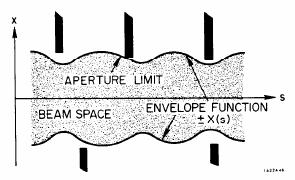
\includegraphics[width=0.8\linewidth]{./Figuras/fig46.jpeg}
	\caption{Radial aperture limit.}
	\label{fig:fig46}
\end{figure}
We have seen in Section~\ref{sec:2.7} that the radial displacement on successive passages of any chosen azimuth varies with time as
\begin{align}
	x = a \sqrt{\beta_1} \cos\omega t.
\end{align}
As we did in Section\ref{sec:5.3} for the energy oscillations we may take the square of the
amplitude factor as a measure of the ``effective energy'' of the oscillations. Let's define
\begin{align}
	W = a^2 \beta_1.
\end{align}
Quantum effects and radiation damping produce slowly varying fluctuations in $W$. The same arguments made in Section~\ref{sec:5.3} can be used again to show that -- in the absence of any aperture limit -- the electrons in a beam will have a distribution of $W$'s according to (see Eq.~\eqref{eq:5.62})
\begin{align}\label{eq:5.120}
	h(W) = \dfrac{N}{\mean{W}}\exp(-W/\mean{W}),
\end{align}
where the mean value $\mean{W}$ is equal to $2\sigma_x^2$ (the function $h(W)$ is defined such
that the number of electrons with ``oscillation energy'' between $W$ and $W + dW$ is $h(W)dW$). The function $h(W)$ is shown by the solid curve in Fig.~\ref{fig:fig47}.
\begin{figure}[!htb]
	\centering
	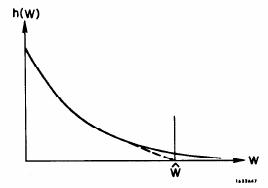
\includegraphics[width=0.8\linewidth]{./Figuras/fig47.jpeg}
	\caption{Distribution of oscillation energies.}
	\label{fig:fig47}
\end{figure}
Now consider what happens when there is an aperture limit that removes any electron for which $W$ exceeds some limiting value $\hat{W}$ -- which we may call ``$W$-peak''. There can be no electrons with $W > \hat{W}$, so the actual distribution $h(W)$ must change for large $W$ to correspond to something like the broken line curve in Fig.~\ref{fig:fig47}. We may think about what is happening in the following way. The quantum effects are continually trying to fill in the ideal distribution by a ``diffusion'' of electrons from the region of small $W$ into the region of large $W$. But each time an electron reaches $\hat{W}$ it is ``wiped off'', so there is a continuous loss out of the tail of the distribution. I would like now to make an estimate of this loss rate.\\
We may make a rough estimate in the following way. We have said that there is a characteristic
 ``relaxation time'' for the quantum fluctuations equal to the damping time constant $\tau_x$. We may guess that there is an ``attempt'' to fill in the tail of the ideal distribution once each damping time. Then the number of electrons lost in each damping time will be equal to the number of electrons in the ideal distribution with $W > \hat{W}$. That number is
\begin{align}
	N(>\hat{W}) = \int_{\hat{W}}^\infty h(W) dW = N \exp(-\hat{W}/\mean{W}).
\end{align}
The electron loss rate will then be estimated by
\begin{align}
	- \dfrac{dN}{dt} \approx \dfrac{N}{\tau_x} \exp(-\hat{W}/\mean{W}),
\end{align}
which would give a quantum lifetime of
\begin{align}\label{eq:5.123}
	\tau_q \approx \tau_x \exp(\hat{W}/\mean{W}).
\end{align}
We would estimate that the lifetime itself depends exponentially on $\hat{W}/\mean{W}$.\\
An exact calculation of $\tau_q$ requires setting up a diffusion equation for $h(W)$ and solving it numerically with the appropriate boundary conditions. I shall not attempt to do this but rather show how a good approximation to the exact result can be obtained.\\
Consider what would be happening in the neighborhood of some particular $W_0$ that is much greater than $\mean{W}$ if there were no aperture limit. The chance of finding any particular
 electron with $W > W_0$ in the ideal distribution is very small. We may expect that if an electron once gets into the tail ($W > W_0$) it is most likely to return rather quickly to the main body of the distribution -- being replaced in the tail by some other unfortunate electron. Consider now the flux of electrons passing through a small zone\footnote{We should think of passage through a ``zone'' so that we may ignore the microscopic fluctuations in the amplitude.} near $W_0$. The electrons which have been populating the tail will be passing to the left through this zone and an equal flux of electrons will (in the stationary state) be passing toward the right through the zone due to abnormal quantum fluctuations (we are neglecting the unlikely events in which an electron leaving the tail would have at that instant an abnormal fluctuation and reenter the tail of the distribution right away).\\
Let's estimate the flux of electrons coming out of the tail. When $W$ is large the ``normal'' energy fluctuations can be neglected in comparison with the rate of decrease of $W$ due to the damping. For any electron the damping gives
\begin{align}\label{eq:5.124}
	\dfrac{dW}{dt} = - \dfrac{2W}{\tau_x},
\end{align}
and the flux of electrons through $W_0$ due to the damping will be
\begin{align}\label{eq:5.125}
	\left\lbrace h(W) \dfrac{dW}{dt} \right\rbrace_{W_0} = \dfrac{2 W_0 h(W_0)}{\tau_x}.
\end{align}
In the absence of an aperture limit the net flux through any $W$ -- and past $W_0$ in particular
 -- must be zero so there would also be an outward flux of electrons quite equal to the inward flux of \eqref{eq:5.125}.\\
Now put in the aperture limit at $\hat{W}$. If it is sufficiently large, the main body of the distribution is little affected. The flux outward through $\hat{W}$ will be unchanged while the return flux will of course, be zero. We have that the flux of \eqref{eq:5.124}, evaluated at $W_0 = \hat{W}$, is also an estimate of the outward flux of lost electrons. The loss rate will be
\begin{align}
	-\dfrac{dN}{dt} = \dfrac{2\hat{W}h(\hat{W})}{\tau_x}.
\end{align}
Using Eq.~\eqref{eq:5.120} for $h(W)$ we obtain,
\begin{align}\label{eq:5.127}
	\tau_q = \dfrac{\tau_x}{2} \dfrac{\mean{W}}{W} \exp \left( \hat{W}/\mean{W} \right).
\end{align}
Remember that $\hat{W}$ and $\mean{W}$ are related to the limiting radial excursion permitted by the aperture (assumed to occur at some azimuth $s_1$) and the rms radial displacement at that azimuth by
\begin{align}
	\hat{W} = \left[ a^2 \beta(s_1) \right]_\text{Max}; && \mean{W} = 2\sigma_x^2(s_1),
\end{align}
with both numbers evaluated at the azimuthal position of the limiting aperture.\\
This result differs from the estimate in Eq.~\eqref{eq:5.123} by the factor $\mean{W}/2\hat{W}$ and gives, therefore, a lifetime smaller by a factor which might be typically 5 or 10. The discrepancy can be explained by arguing that the ``relaxation time'' is shorter by this factor for the population of the tail of the distribution than for the main body of it -- which is understandable since a large fluctuation has a better chance of dominating the radiation damping if it accumulates during a relatively short time span. Although Eq.~\eqref{eq:5.127} was derived by making some approximations whose quantitative significance we have not tried to estimate, the same result has been obtained by more sophisticated -- although still approximate -- techniques (see \cite{5}, \cite{15}).\\
In our derivation of the quantum lifetime we have assumed that the radial fluctuations were due solely to betatron oscillations. As we have seen in Section~\ref{sec:5.5} however, the radial beam spread has contributions from both the betatron and energy oscillations. And the analysis is complicated by the fact that the two components have different damping time constants. I shall not attempt to refine the calculation but settle for the following comments. The two damping time constants are not very different -- usually within a factor of two of each other. It is then clear that Eq.~\eqref{eq:5.125} will give a reasonable approximation if we use for $\sigma_x^2$ the total mean-square beam spread and for $\tau_x$ some value between the betatron and synchrotron damping time constants. Or alternatively we may get a ``safe'' estimate of $\tau_q$ -- that is a lower limit -- by using for $\tau_x$ the smaller of the two time constants.\\
The quantum lifetime increases approximately exponentially with the square of the limiting radial excursion -- an exceedingly rapid variation. There is then, a rather precise criterion
 for the aperture required. If the aperture is just a little bit too small the lifetime will be disastrously short, but if it is a little larger than necessary the lifetime will be astronomically large and will be of no consequence\footnote{Since other loss mechanisms
 will then dominate.}. The ``critical'' aperture limit occurs at about
\begin{align}
	\dfrac{|x_\text{max}|}{\rho_x} = 6\sigma_x.
\end{align}
which gives $\hat{W}/\mean{W} \approx 18$ and from Eq.~\eqref{eq:5.120},
\begin{align}
	\tau_q = \dfrac{\tau_x}{36} e^{18} \approx 1.5 \times 10^6 \tau_x.
\end{align}
Since $\tau_x$ is typically about 0.1 sec, the critical aperture gives a quantum lifetime
of about one day. Other effects such as gas scattering usually give lifetimes of several hours and the filling time (time to store an operating beam) is generally a fraction of an hour, so a quantum lifetime of one day is quite ``safe''. We can understand the ``rule-of-thumb'' that the full aperture must be at least 12 times the standard deviation $\sigma_x$ of the radial distribution. A similar rule clearly holds for the vertical aperture.

    \section{Beam Lifetime from Energy Oscillations} \label{eq:5.8}

In the preceding section we have examined the loss of electrons due to abnormal fluctuations in the amplitudes of the radial oscillations. Loss of electrons from a stored beam will also occur when abnormal fluctuations in the energy oscillations result in energy excursions so large that they can no longer be contained within the energy aperture that is determined by the radio frequency accelerating system.\\
In Section~\ref{sec:3.6} we saw that the energy oscillations correspond to the motion of an ideal particle in a potential well, one of whose walls is a potential "hill" of limited height. The situation was described by Fig. 36(b), a part of which is redrawn in Fig.~\ref{fig:fig48}(a). The horizontal coordinate is the time displacement associated with the energy oscillations and the vertical coordinate is a fictitious "potential energy" of the oscillation. The corresponding "kinetic energy" is
\begin{align} \label{eq:5.131}
	\dfrac{1}{2}\left( \dfrac{d\tau}{dt} \right)^2 = \dfrac{\alpha^2}{2} \left( \dfrac{\epsilon}{E_0} \right)^2.
\end{align}
where $\epsilon$ is the instantaneous energy deviation of the real energy oscillation.

\begin{figure}[!htb]
	\centering
	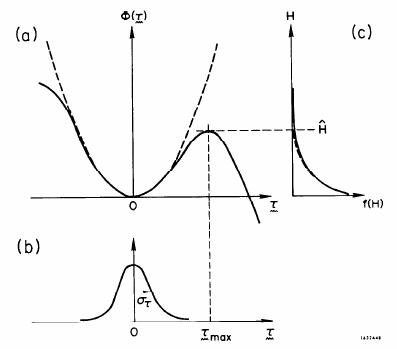
\includegraphics[width=0.8\linewidth]{./Figuras/fig48.jpeg}
	\caption{Quantum spread in the energy oscillations.}
	\label{fig:fig48}
\end{figure}

Suppose we let $H$ represent the "total oscillation energy" -- that is, the sum of the "potential
 energy" and the "kinetic energy" of Eq.~\eqref{eq:5.131} --
\begin{align}
	H = \Phi(\tau) + \dfrac{\alpha^2}{2} \left( \dfrac{\epsilon}{E_0} \right)^2,
\end{align}
($\Phi$ is taken to be zero at the bottom of the potential well) During the oscillation of any particular electron the "potential energy" reached at the maximum of $\tau$ is equal to $H$. And the peak "kinetic energy" -- which occurs as the electron passes $\tau = 0$ -- is also equal to %
$H$, so
\begin{align}
	H = \dfrac{\alpha^2}{2} \dfrac{\epsilon^2}{E_0^2}.
\end{align}
where $\hat{\epsilon}$ is the peak value of $\epsilon$ during its oscillation. An electron is captured in a stable energy oscillation if $H$ is less than $\Phi_\text{max}$, the maximum height of the potential well (See Section~\ref{sec:3.6}). Otherwise it will be lost.\\
In Sections~\ref{sec:5.2} and \ref{sec:5.3} we have examined the quantum-induced energy oscillations under the assumption that they were ideally linear -- which would correspond to the ideal parabolic potential-well indicated by the broken line in Fig.~\ref{fig:fig48}(a). Under these assumptions, the distribution of time displacements in a stored bunch of electrons would be as the Gaussian function drawn in Fig.~\ref{fig:fig48}(b) - whose standard deviation $\sigma_\tau$ was evaluated in Section~\ref{sec:5.4}.\\
We have also seen that the energy fluctuations yield an exponential distribution in the square of the amplitude of the energy oscillations -- as described by Eq.~\eqref{eq:5.62}. The quantity $W$ used there is just the square of the amplitude (of the oscillation in $\epsilon$) and is therefore, proportional to the "total energy" $H$. In fact,
\begin{align}
	H = \dfrac{\alpha^2}{2 E_0^2}W.
\end{align}
It follows that the distribution over $H$ for the electrons stored in a bunch is also exponential. Specifically, if we let $f(H)dH$ represent the number of electrons with "total oscillation energies" between $H$ and $H + dH$, then a direct translation of Eq.~\eqref{eq:5.62} gives
\begin{align}
	f(H)dH = \dfrac{N}{\mean{H}} \exp \left( -H/\mean{H} \right),
\end{align}
where
\begin{align}
	\mean{H} = \dfrac{\alpha^2}{2 E_0^2} \mean{W} = \dfrac{\alpha^2}{E_0^2} \sigma_\epsilon^2.
\end{align}
This distribution in oscillation energies is shown in Fig.~\ref{fig:fig48}(c).\\
The real situation must evidently be different. Any electron whose time displacement once exceeds $\tau_\text{max}$, the value of $\tau$ at the top of the actual potential hill -- or equivalently, one whose "oscillation energy" $H$ exceeds $\Phi_\text{max}$ -- will be lost from the stored bunch. As we saw in the preceding section for the radial oscillations, we must expect that the actual distributions will fall to zero at $\tau_\text{max}$ -- and therefore at $H = \hat{H} = \Phi_\text{max}$. And there will be a continuous loss of electrons due to diffusion
 out of the tail of the distribution.\\
The situation here is similar to the one discussed in the preceding section, which would correspond to a parabolic potential well which is suddenly truncated at $\tau_\text{max}$. The smooth rounding of the potential maximum will have a somewhat different effect on the comportment of the distribution of electrons near the edge of the distribution. One may expect however, that so long as $\tau_\text{max} >> \sigma_\tau$, the rate of loss of electrons may be estimated in the same way for both situations.\\
Without repeating the argument here, we may write the result which corresponds to Eq.~\eqref{eq:5.127}, translated to the case of the energy oscillations,
\begin{align}
	\tau_q = \dfrac{\tau_\epsilon}{2} \dfrac{e^\xi}{\xi},
\end{align}
with
\begin{align}
	\xi = \dfrac{\hat{H}}{\mean{H}} = \dfrac{\Phi_\text{max}}{\mean{H}}.
\end{align}
The height $\Phi_\text{max}$ of the potential maximum can be evaluated by performing the integration of Eq.~\eqref{eq:3.53} -- or for a sinusoidal rf voltage, from Eq.~\eqref{eq:3.58}.\\
The potential $\Phi_\text{max}$ was introduced in order to obtain the magnitude of the "aperture"
 of the energy oscillations. It is related to the maximum acceptable energy deviation $\epsilon_\text{max}$ -- see Eq.~\eqref{eq:5.57} --
\begin{align}
	\Phi_\text{max} = \dfrac{\alpha^2}{2} \left( \dfrac{\epsilon_\text{max}}{E_0} \right)^2.
\end{align}
So $\xi$ has the conceptually simple form
\begin{align}
	\xi = \dfrac{\epsilon_\text{max}^2}{2\sigma_\epsilon^2}.
\end{align}
The potential $\Phi_\text{max}$ and, therefore, the number $\xi$ depends on the magnitude of the rf voltage which must always be sufficiently large to give a quantum lifetime greater than the desired storage time of the beam. Typically $\xi$ must be at least as large as 18 or so, requiring that $\epsilon_\text{max}/\sigma_\epsilon$ be about 6.\\
For the particular (but very common) case of a storage ring with an isomagnetic guide field and a sinusoidally varying rf voltage, the parameter $\xi$ can be expressed rather simply in terms of the ring parameters. Bringing together the results obtained in earlier sections for $\epsilon_\text{max}$ and $\sigma_\epsilon$ you can show that
\begin{align}
	\xi = \dfrac{J_\epsilon E_0}{\alpha k E_1} F(q) && \text{(isomag.)}.
\end{align}
where $E_1$ is a constant with the dimensions of an energy:
\begin{align}
	E_1 = \dfrac{3mc^2 C_q}{2 r_e} = \dfrac{55 \sqrt{3}}{64} \dfrac{\hslash c}{r_e} \approx 1.08 \times 10^8 \text{eV},
\end{align}
and $F(q)$ is the energy aperture function which was defined in Eq.~\eqref{eq:3.60} and is shown in Fig.~\ref{fig:fig38}. The parameter $q$ is the rf overvoltage -- namely the ratio of the peak rf voltage to the energy lost in one turn. For large overvoltages $F(q)$ is approximately $(2q- \pi)$ and the quantum lifetime increases exponentially with increasing rf voltage.\\
Notice that in a storage ring with a given guide field (that is with a fixed $\alpha$,
$J_\epsilon$, $\tau_\epsilon$ and $E_0$) the overvoltage required for any particular quantum lifetime (that is for a particular $\xi$) depends on the harmonic number $k$ of the rf system. For large harmonic numbers the overvoltage required varied approximately as $\sqrt{k}$.




\chapter{Appendices} \label{ch:app}
    \section{Basics of Charged Particles in Magnetic Fields} \label{sec:BasicsMagField}

A particle of charge $q$ with velocity $\bm{v}$ in the presence of a magnetic vector field $\bm{B} = \bm{B}(\bm{r})$ experiences a Lorentz force 
\begin{equation}
\bm{F} = q \; \bm{v} \times \bm{B},
\end{equation}
In the case of the electron, $q=-e$, where $e = 1.6021766208(98)\times10^{-19}\;C$ is the elementary charge fundamental constant. If the magnetic field is colinear with the velocity, the force vanishes. Moreover, the Lorentz force in a pure magnetic field does no work on the charged particle, as can be mathematically derived,
\begin{eqnarray}
\bm{F} \cdot d\bm{r} &=& q \; \left( \bm{v} \times \bm{B} \right) \cdot d\bm{r} \nonumber \\
                     &=& q \; \left( d\bm{r} \times \bm{v} \right) \cdot \bm{B} = q \; dt \left( \bm{v} \times \bm{v} \right) \cdot \bm{B} \\
                     &=& 0 \nonumber,
\end{eqnarray}
since the infinitesimal displacement vector is colinear with the velocity. As a consequence, the speed $v$ and the mechanical energy $E$ of the relativistic particle,
\begin{equation}
E = m c^2 = \gamma m_0 c^2 = \frac{m_0 c^2}{\sqrt{1-(v/c)^2}}
\end{equation}
are conserved. Therefore, its relativistic mass is constant and the time derivative of the linear momentum is proportional to the acceleration:
\begin{equation}
\frac{d\bm{p}}{dt} = m \frac{d\bm{v}}{dt} = q \; \bm{v} \times \bm{B}. 
\end{equation}
This equation describes how the particle velocity evolves in the presence of a magnetic field. 

Since the magnitude $v$ of the velocity $\bm{v} = v\bm{\hat{v}}$ is a constant of motion, the above equation can be rewritten for the velocity versor $\bm{\hat{v}}$. Also, we can change the independent variable from time $t$ to the trajectory arc length $\ell$ using $v = d\ell/dt$. The rate at which the direction of movement $\bm{\hat{v}}$ changes with the arc length is then given by
\begin{equation}
\frac{d\bm{\hat{v}}}{d\ell} = \frac{qc}{\beta E} \bm{\hat{v}} \times \bm{B},
\end{equation}
where $\beta \equiv v/c$. By defining the magnetic rigidity $R_m=R_m(E)$ as
\begin{equation}
R_m = p/q = \frac{\beta E}{qc},
\end{equation}
it is possible to rewrite the equation for $d\bm{\hat{v}}/d\ell$ in a concise way as
\begin{equation}
\label{eq:lorentz_versor}
\frac{d\bm{\hat{v}}}{d\ell} = \frac{1}{R_m} \bm{\hat{v}} \times \bm{B}.
\end{equation}

Assume a trajectory direction whose projection onto the plane normal to a field $\bm{B} = B\bm{\hat{y}}$ makes a angle $\theta=\theta(s)$ with respect to $\bm{\hat{z}}$,
\begin{equation}
\bm{\hat{v}} = \hat{v}_{\parallel}\cos{\theta} ~ \bm{\hat{z}} + \hat{v}_{\parallel}\sin{\theta} ~ \bm{\hat{x}} + \hat{v}_{\perp} ~ \bm{\hat{y}},
\end{equation}
Equation (\ref{eq:lorentz_versor}) is then solved for this case:
\begin{align*}
\frac{d}{d\ell}(\hat{v}_{\parallel}\cos{\theta} ~ \bm{\hat{z}} + \hat{v}_{\parallel}\sin{\theta} ~ \bm{\hat{x}} + \hat{v}_{\perp} ~ \bm{\hat{y}}) = \frac{1}{R_m} (\hat{v}_{\parallel}\cos{\theta} ~ \bm{\hat{z}} + \hat{v}_{\parallel}\sin{\theta} ~ \bm{\hat{x}} + \hat{v}_{\perp} ~ \bm{\hat{y}}) \times (B\bm{\hat{y}})
\end{align*}

In the ultrarrelativistic context considered here, the particle is moving along the longitudinal direction close to \bm{$\hat{z}}$, then $\hat{v}_{\parallel}$ not significantly changes with $\ell$ in comparison with the angle and the transverse component. The velocity in the $\bm{\hat{y}}$ direction remains unchanged whereas the two other components reduce to a single expression for the evolution of the deflected angle of the particle along the trajectory:
\begin{equation}
\frac{d\theta}{d\ell}  = -\frac{B}{R_m}. 
\end{equation}

This last equation shows that the deflection angle per unit path length is the ratio between the magnetic field intensity and the magnetic rigidity of the particle, which depends solely on its energy. The integral form of the equation, used to compute the angular displacement accumulated along a path $\Gamma$, reads
\begin{equation}
\label{equ:deflection_angle}
\Delta \theta = -\frac{1}{R_m} \int_{\Gamma} B \; d\ell.
\end{equation}

A deflection in angle comes with a bending radius $\rho$ of curvature, conventionaly considered positive when the rotation direction is in the clockwise sense and negative when it is counter-clockwise. Together with the convention of angles measured counter-clockwise, the geometry of the problem is syntetized by the following equation:
\begin{equation}
    d\theta = -\frac{dl}{\rho} = -G dl
\end{equation}
where the curvature function $G$ is defined as
\begin{align}
    G = \frac{1}{\rho}
\end{align}

This relation now leads to an interesting expression for the magnetic rigidity
\begin{equation}
\label{eq:rigidity}
    B\rho = {R_m} = p/q.
\end{equation}
This parameter relates the geometry of the magnetic problem, as shown in the left hand side of the equation, with the caracteristics of the particle, the right hand side. The larger the magnetic rigidity of the particle is -- hence the higher its energy is -- the more difficult it is for a given magnetic field amplitude to bend the particle trajectory and, therefore, the larger the bending radius is.

For a numerical example, consider the 3 GeV beam at SIRIUS storage ring. Electrons in the beam have, for this nominal energy, a magnetic rigidity of approximately 10 T$\cdot$m. In order to deflect them by a complete turn, 360 degrees, the integrated field experienced must be of $2\pi R_m \approx$ 62.8 T$\cdot$m. Typical magnetic fields in dipoles are around 1 T, which means that if SIRIUS were to be build with such uniform field dipoles it would require exactly 62.8 meters of them.

In general case of an arbitrary transverse field $\bm{B}=B_x\bm{\hat{x}}+B_y\bm{\hat{y}}$ its useful to express the movement direction of the particle close to the longitudinal $\bm{\hat{z}}$ using the small angles approximation.
\begin{align}
    \bm{\hat{v}} &= \sin{\theta}\cos{\phi} ~ \bm{\hat{x}} + \sin{\theta}\sin{\phi} ~ \bm{\hat{y}} + \cos{\theta} ~ \bm{\hat{z}} \nonumber \\
    \bm{\hat{v}} &= \theta\cos{\phi} ~ \bm{\hat{x}} + \theta\sin{\phi} ~ \bm{\hat{y}} + \left(1-\frac{1}{2}\theta^2\right)\bm{\hat{z}} \nonumber \\
    \bm{\hat{v}} &= \theta_x ~ \bm{\hat{x}} + \theta_y ~ \bm{\hat{y}} + \left(1-\frac{\theta_x^2+\theta_y^2}{2}\right)\bm{\hat{z}}
\end{align}

The Eq.(\ref{eq:lorentz_versor}) is solved again for the deflection angles at the horizontal and vertical planes:
\begin{equation}
    \frac{d\theta_x}{d\ell}  = - \frac{B_y}{R_m} \quad ; \quad \frac{d\theta_y}{d\ell}  = \frac{B_x}{R_m}
\end{equation}

Explicitly, the radius of curvatures at each plane are
\begin{equation}
    \rho_{x,y}=\pm \frac{R_m}{B_{y,x}}.
\end{equation}
Notice that the radius at the vertical has opposite sign of the one in the horizontal.

For the ultrarrelativistic electrons, $\beta\approx 1$ and $q=-e$, then the radii of their orbit are:
\begin{equation}
    G_{x,y} = \frac{1}{\rho_{x,y}} = \mp \frac{ec}{E}B_{y,x}
\end{equation}

    \section{Floquet Theorem} \label{sec:FloquetTheorem}

Considering Hill's equation,
\begin{align}\label{eq:Hill}
	x''+K(s)x=0,
\end{align}
where $K(s)$ is a piecewise continuous function in every finite interval and that it is periodic with minimal period $L$. According to Floquet theorem, any solution can be written as the linear combination of the following independent solutions:
\begin{align*}
	x_1(s) &= \zeta(s) e^{i \varphi(s)}, \\
	x_2(s) &= \zeta(s) e^{-i \varphi(s)},
\end{align*}
where the functions $\zeta$ and $\varphi$ satisfy the following periodic boundary conditions for all $s$, and $\nu$ represents a constant phase advance:
\begin{align*}
	\zeta(s) = \zeta(s+L), && \varphi(s+L)-\varphi(s) = 2\pi \nu.
\end{align*}
Plugging this result in equation \eqref{eq:Hill}, it results in a system of differential equations:
\begin{align*}
	\begin{cases}
		2 \zeta' \varphi' + \zeta \varphi'' = 0, \\
		\zeta'' + K(s)\zeta - \zeta \varphi'^2 = 0.
	\end{cases}
\end{align*}
The first differential equation can be written as
\begin{align*}
	\dfrac{d}{ds}( \varphi' \zeta^2 ) &= 0.
\end{align*}
Then, it is easy to show that
\begin{align}
	\varphi'(s) &= \dfrac{C}{\zeta^2(s)},
\end{align}
where $C$ is a constant, which can be set equal to $1$ without loss of generality.
Then, the second equation becomes
\begin{align}
	\zeta'' + K(s) \zeta - \dfrac{1}{\zeta^3}=0.
\end{align}

If the initial conditions $x(0)$, $x'(0)$ are real numbers and $K(s)$ is a real valued function, then a general form of the solution can be written as
\begin{align}
	x(s) = a \zeta(s) \cos(\varphi(s) - \vartheta),
\end{align}
where $a$ and $\vartheta$ are constants determined by the initial conditions.
    \section{Tune Shift with Gradient Errors}\label{sec:dtune_grad_err}

In order to deduce the tune shift with a gradient error, let us use the transfer matrix formalism. From Eq.~\eqref{eq:2.37}, the one-turn transfer matrix is given by,
\begin{align*}
	\boldsymbol{M}(0,L)
    &= \begin{bmatrix}
	C(0,L) & S(0,L)\\
	C'(0,L) & S'(0,L)
	\end{bmatrix}
\end{align*}
 Since we know that
\begin{align*}
	C(0,L) &= \cos(2\pi\nu) - \dfrac{\beta'}{2} \sin(2\pi\nu),\\
    S'(0,L) &= \dfrac{\beta'}{2} \sin(2\pi\nu) + \cos(2\pi\nu);
\end{align*}
it is easy to see that $\Tr [\boldsymbol{M}(0,L)] = 2\cos(2\pi\nu)$, so it is possible to find the tune $\nu$, from the trace of the one-turn transfer matrix.
If we have a quadrupole perturbation at $s=0$ (without loss of generality), we may represent it with the transfer matrix of the quadrupole, see Table.~\ref{tab:tab1}.\\
Since this perturbation resides in a element of length $\Delta s$, we shall use the thin lenses approximation ($\Delta s$ small, while keeping $k\Delta s$ a constant), as follows
\begin{align}
	\boldsymbol{M}_k &=
	\begin{bmatrix}
			\cos(\sqrt{k}\Delta s) & \frac{1}{\sqrt{k}}\sin(\sqrt{k}\Delta s)\\
			-\sqrt{k}\sin(\sqrt{k}\Delta s) & \cos(\sqrt{k}\Delta s)
	\end{bmatrix}\\
    & \approx
    \begin{bmatrix}
			1 & 0\\
			-k \Delta s & 1
	\end{bmatrix}.
\end{align}
This approximation is valid for $k < 0$ too. The new one-turn matrix is given by $\boldsymbol{M}'(0,L) = \boldsymbol{M}(0,L) \cdot \boldsymbol{M}_k$. As we have just seen, the new tune can be found by calculating $\Tr[\boldsymbol{M}'(0,L)]$. Using the values of $C(0,L)$ and $S'(0,L)$ given above and $S(0,L) = \beta \sin(2\pi\nu)$, the reader can find that
\begin{align}
	\Tr[\boldsymbol{M}'(0,L)] = 2\cos(2\pi\nu) - \beta k \Delta s \sin(2\pi\nu).
\end{align}
Let $\nu + \Delta\nu$ be the new tune, then
\begin{align}
	2\cos(2\pi(\nu+\Delta\nu)) = 2\cos(2\pi\nu) - \beta k \Delta s \sin(2\pi\nu).
\end{align}
Supposing that $\Delta\nu$ is sufficiently small, since $\Delta s$ is sufficiently small, we may use the relation
\begin{align*}
	\cos(2\pi(\nu+\Delta\nu)) \approx \cos(2\pi\nu) - 2\pi\Delta\nu\sin(2\pi\nu),
\end{align*}
to deduce that
\begin{align}
	\Delta\nu \approx \dfrac{1}{4\pi}\beta k \Delta s.
\end{align}
Supposing this effect occurs in the whole ring (and using the linear approximation), we may sum up all $\Delta\nu$ contributions caused by several $k(s)$ in each $\Delta s$ of the ring, obtaining then, the total tune variation
\begin{align}
	\Delta\nu = \dfrac{1}{4\pi}\oint \beta(s) k(s) ds.
\end{align}

    \section{Horizontal Damping}\label{sec:hor_damping}

The expressions for the betatron displacements are given by

\begin{align}
x_\beta &= A\sqrt{\beta} \cos\varphi, \\
x_\beta'& = - A\dfrac{1}{\sqrt{\beta}} \left(\alpha\cos\varphi + \sin\varphi\right).
\end{align}

The amplitude $A$ (action) satisfies the relation $A^2 = \gamma x_\beta^2 + 2\alpha x_\beta x_\beta' + \beta x_\beta'^2$, therefore

\[
A\delta A = \gamma x_\beta \delta x_\beta + \alpha \left(x_\beta \delta x_\beta' + x_\beta' \delta x_\beta\right)  + \beta x_\beta'\delta x_\beta'.
\]

Since $\delta x = \delta x' = 0$ we obtain $\delta x_\beta = - \eta \delta E / E_0$ and $\delta x_\beta' = - \eta' \delta E / E_0$, then

\begin{equation}
A\delta A = -\dfrac{\delta E}{E_0} \left(\gamma x_\beta \eta + \alpha \left(x_\beta \eta' + x_\beta' \eta\right)  + \beta x_\beta'\eta'\right).
\label{eq:amp}
\end{equation}

We must evaluate $\delta E$ along the off-energy orbit. Since $\delta E = P_\gamma \delta l / c$ and $\delta l = -(1 + x / \rho_s) \delta s$
(the minus sign in $\delta s$ comes from the fact that in the emission process the path length is decreasing instead of increasing as in \eqref{eq:2.15}), thus we obtain

\begin{equation}
\delta E = -\dfrac{P_\gamma \delta s}{c} \left(1 + \dfrac{x}{\rho_s}\right).
\label{eq:energy_off}
\end{equation}

Notice that since $x = x_\beta + x_\delta$, when \eqref{eq:energy_off} is inserted into \eqref{eq:amp} the terms $x_\delta x_\beta$ and $x_\delta x_\beta'$
will be zero when averaged over betatron oscilations, then we can write down $(1 + x/\rho_s) = (1 + x_\beta / \rho_s)$. Then we obtain

\[
A\delta A = \dfrac{P_\gamma \delta s}{c E_0 \rho_s} \left(\gamma x_\beta^2 \eta + \alpha \left(x_\beta^2 \eta' + x_\beta' x_\beta  \eta\right)  + \beta x_\beta' x_\beta \eta'\right).
\]

From the expressions for betatron displacement we obtain the average of each term: $\langle x_\beta ^2 \rangle = A^2 \beta /2$ and $\langle x_\beta' x_\beta  \rangle =  - A^2 \alpha /2$.
Then we calculate the average of amplitude variation as (assuming an isomagnetic field $\rho_s = \rho_0$)

\[
A\Delta A = \dfrac{ A^2 U_0}{2 E_0 \rho_0} \left(\gamma \beta \eta + \alpha \beta \eta' - \alpha^2\eta  - \alpha \beta  \eta'\right).
\]

Remember that $\gamma\beta = 1 + \alpha^2$, therefore

\begin{equation}
\dfrac{\Delta A}{A} = \dfrac{U_0 \eta }{2 E_0 \rho_0}
\end{equation}

    \section{Quantum radiation discussion} \label{sec:QuantumRadiation}

In this appendix chapter, we shall elaborate the discussion covered in Section \ref{sec:5.1}. First of all, let us (re-)define our variables:
\begin{itemize}
\item $U_i$ is the random variable that represents the energy emitted by the $i$-th quantum event, we assume that the sequence $(U_i)_{i\geq0}$ is i.i.d. (independent and identically distributed);
\item $N(u)$ is the random variable representing the density of number of quantum events at energy $u$ that happens in a unit time;
\item $n(u) = \mathbb{E}[N(u)]$ is the mean number density function of quanta emitted per unit time with energy $u$;
\item $M = \int_0^\infty N(u)du$ is the random variable representing the total number of quantum events that happens in a unit time;
\item $\mathscr{N} = \mathbb{E}[M] = \int_0^\infty n(u) du$ is the mean number of quanta emitted per unit time;
\end{itemize}
where $\mathbb{E}$ stands for the expected value operator. The i.i.d. supposition over the sequence of random quantum events is reasonable, since the mean quantum energy emitted is much smaller than the energy of the electron. Another assumption is that the quantities $\rho$ and $\gamma$ does not change significantly in a  time-scale of a quantum event, which is approximately $\rho/\gamma^3 c$. \\
Using the above definitions, it is easy to see that the expected total power lost by quanta events (radiation) is given by
\begin{align}
	P_\gamma &= \mathbb{E}\left[ \sum_{i=1}^{M} U_i \right],
\end{align}
Separating this sums by energy, we can write that
\begin{align*}
	P_\gamma &= \mathbb{E}\left[ \int_0^\infty N(u) u du \right]\\
    		&= \int_0^\infty u \mathbb{E}[N(u)] du\\
            &= \int_0^\infty u n(u) du \bydef \mathscr{N} \mean{u}.
\end{align*}

Now, we shall justify more rigorously Eq.~\eqref{eq:5.26}. As shown in equation \eqref{eq:5.25}, the probable change in the amplitude squared due to one single quantum event is $u^2$. So the probable change after $m$ quantum events is
\begin{align}
	\mean{\delta A^2} = u_1^2 + u_2^2 + ... + u_m^2,
\end{align}
where $u_i$ is the energy emitted by the $i$-th quantum event. However, the emitted energy is not deterministic, so it is necessary a different approach to calculate $\mean{\delta A^2}$.
As we did for $P_\gamma$, $\mean{\delta A^2}$ can be written as
\begin{align}
	\mean{\delta A^2} = \mathbb{E} \left[ \sum_{i=1}^M U_i^2 \right],
\end{align}
Then, doing the same steps as before, we may write
\begin{align*}
	\mean{\delta A^2} &= \mathbb{E}\left[ \int_0^\infty N(u) u^2 du \right]\\
    		&= \int_0^\infty u^2 \mathbb{E}[N(u)] du\\
            &= \int_0^\infty u^2 n(u) du \bydef \mathscr{N} \mean{u^2}.
\end{align*}
It is important to remember that if the mean emitted energy $P_\gamma$ were comparable to the electron energy $E$, then the variables $U_i$ and $M$ would not be independent and our expressions would be much more complicated to calculate, since it would not be possible to integrate independently in the energy, \textit{i.e.}, the density numbers of emissions for a given energy would affect one another.

\bibliographystyle{plain}
\bibliography{ref}

\end{document}
